\documentclass[twoside]{book}

% Packages required by doxygen
\usepackage{fixltx2e}
\usepackage{calc}
\usepackage{doxygen}
\usepackage[export]{adjustbox} % also loads graphicx
\usepackage{graphicx}
\usepackage[utf8]{inputenc}
\usepackage{makeidx}
\usepackage{multicol}
\usepackage{multirow}
\PassOptionsToPackage{warn}{textcomp}
\usepackage{textcomp}
\usepackage[nointegrals]{wasysym}
\usepackage[table]{xcolor}

% Font selection
\usepackage[T1]{fontenc}
\usepackage[scaled=.90]{helvet}
\usepackage{courier}
\usepackage{amssymb}
\usepackage{sectsty}
\renewcommand{\familydefault}{\sfdefault}
\allsectionsfont{%
  \fontseries{bc}\selectfont%
  \color{darkgray}%
}
\renewcommand{\DoxyLabelFont}{%
  \fontseries{bc}\selectfont%
  \color{darkgray}%
}
\newcommand{\+}{\discretionary{\mbox{\scriptsize$\hookleftarrow$}}{}{}}

% Page & text layout
\usepackage{geometry}
\geometry{%
  a4paper,%
  top=2.5cm,%
  bottom=2.5cm,%
  left=2.5cm,%
  right=2.5cm%
}
\tolerance=750
\hfuzz=15pt
\hbadness=750
\setlength{\emergencystretch}{15pt}
\setlength{\parindent}{0cm}
\setlength{\parskip}{3ex plus 2ex minus 2ex}
\makeatletter
\renewcommand{\paragraph}{%
  \@startsection{paragraph}{4}{0ex}{-1.0ex}{1.0ex}{%
    \normalfont\normalsize\bfseries\SS@parafont%
  }%
}
\renewcommand{\subparagraph}{%
  \@startsection{subparagraph}{5}{0ex}{-1.0ex}{1.0ex}{%
    \normalfont\normalsize\bfseries\SS@subparafont%
  }%
}
\makeatother

% Headers & footers
\usepackage{fancyhdr}
\pagestyle{fancyplain}
\fancyhead[LE]{\fancyplain{}{\bfseries\thepage}}
\fancyhead[CE]{\fancyplain{}{}}
\fancyhead[RE]{\fancyplain{}{\bfseries\leftmark}}
\fancyhead[LO]{\fancyplain{}{\bfseries\rightmark}}
\fancyhead[CO]{\fancyplain{}{}}
\fancyhead[RO]{\fancyplain{}{\bfseries\thepage}}
\fancyfoot[LE]{\fancyplain{}{}}
\fancyfoot[CE]{\fancyplain{}{}}
\fancyfoot[RE]{\fancyplain{}{\bfseries\scriptsize Generated by Doxygen }}
\fancyfoot[LO]{\fancyplain{}{\bfseries\scriptsize Generated by Doxygen }}
\fancyfoot[CO]{\fancyplain{}{}}
\fancyfoot[RO]{\fancyplain{}{}}
\renewcommand{\footrulewidth}{0.4pt}
\renewcommand{\chaptermark}[1]{%
  \markboth{#1}{}%
}
\renewcommand{\sectionmark}[1]{%
  \markright{\thesection\ #1}%
}

% Indices & bibliography
\usepackage{natbib}
\usepackage[titles]{tocloft}
\setcounter{tocdepth}{3}
\setcounter{secnumdepth}{5}
\makeindex

% Hyperlinks (required, but should be loaded last)
\usepackage{ifpdf}
\ifpdf
  \usepackage[pdftex,pagebackref=true]{hyperref}
\else
  \usepackage[ps2pdf,pagebackref=true]{hyperref}
\fi
\hypersetup{%
  colorlinks=true,%
  linkcolor=blue,%
  citecolor=blue,%
  unicode%
}

% Custom commands
\newcommand{\clearemptydoublepage}{%
  \newpage{\pagestyle{empty}\cleardoublepage}%
}

\usepackage{caption}
\captionsetup{labelsep=space,justification=centering,font={bf},singlelinecheck=off,skip=4pt,position=top}

%===== C O N T E N T S =====

\begin{document}

% Titlepage & ToC
\hypersetup{pageanchor=false,
             bookmarksnumbered=true,
             pdfencoding=unicode
            }
\pagenumbering{alph}
\begin{titlepage}
\vspace*{7cm}
\begin{center}%
{\Large Hardware Development of F\+I\+Nken I\+II quadcopter \\[1ex]\large V1.\+0 }\\
\vspace*{1cm}
{\large Generated by Doxygen 1.8.13}\\
\end{center}
\end{titlepage}
\clearemptydoublepage
\pagenumbering{roman}
\tableofcontents
\clearemptydoublepage
\pagenumbering{arabic}
\hypersetup{pageanchor=true}

%--- Begin generated contents ---
\chapter{Software Development for F\+I\+Nken}
\label{index}\hypertarget{index}{}\hypertarget{index_intro_sec}{}\section{Introduction}\label{index_intro_sec}
Our project is to develop hardware for the F\+I\+Nken 3 robots.

We have designed the P\+C\+Bs where the reference link is given below for the further details \href{https://github.com/ovgu-FINken/DE-HW-Hardware/wiki}{\tt Hardware wiki link}

This document mainly focused on the software part.

Currently the F\+I\+Nken I\+II is the newest generation of our copters with more power, better communication and more sensors 

{\bfseries Specifications \+:}


\begin{DoxyEnumerate}
\item Optical flow sensor with sonar ranging towards ground (Optional\+: Infrared distance sensor towards ground)
\item Tower of 4 sonar ranging sensor
\item 802.\+15.\+4 based phase-\/difference ranging between copters and anchors
\item Paparazzi\+U\+AV board (Lisa/M 2.\+1) -\/ with floating point support
\item 802.\+15.\+4 Communication Module to communicate to ground station and between copters
\end{DoxyEnumerate}\hypertarget{index_Software_sec}{}\section{Software Development}\label{index_Software_sec}


\hypertarget{index_comp_sec}{}\subsection{Components used in our project}\label{index_comp_sec}




List of components is provided below\+:


\begin{DoxyEnumerate}
\item Optical flow sensor with sonar ranging towards ground
\item 8 Sonars ranging sensors
\item Paparazzi\+U\+AV board
\item R\+GB L\+E\+Ds
\item Illuminating Sensor
\item S\+T\+M32\+F44\+R\+E\+T6 Micro controller 

 
\end{DoxyEnumerate}\hypertarget{index_prog_sec}{}\subsection{Programming language and installation guide for using in Linux}\label{index_prog_sec}




We programmed in C\+Lion using Mbed libraries in C++ language. For using mbed libraries, mbed cli needs to install for exporting into I\+DE.

Below is the procedure as follows\+:


\begin{DoxyEnumerate}
\item Install Python v2.\+7
\item Install Git and Mercurial
\item Install G\+NU A\+RM Embedded Toolchain Step0\+: Remove previous version of toolchains, if needed \char`\"{}sudo apt-\/get remove gcc-\/arm-\/none-\/eabi\char`\"{} \char`\"{}sudo apt-\/get remove g++-\/arm-\/linux-\/gnueabi\char`\"{} \char`\"{}sudo apt-\/get remove binutils-\/arm-\/none-\/eabi\char`\"{} Step1\+: Inside Ubuntu, open a terminal and input \char`\"{}sudo add-\/apt-\/repository ppa\+:team-\/gcc-\/arm-\/embedded/ppa\char`\"{}
\end{DoxyEnumerate}

Step2\+: Continue to input \char`\"{}sudo apt-\/get update\char`\"{}

Step3\+: Continue to input to install toolchain \char`\"{}sudo apt-\/get install gcc-\/arm-\/embedded\char`\"{}
\begin{DoxyEnumerate}
\item Install mbed-\/cli \char`\"{}sudo pip install mbed-\/cli\char`\"{}
\item Get the program
\item Select tollchain in mbed-\/cli. Run in folder my\+\_\+program/mbed\+\_\+os \char`\"{}mbed config -\/-\/global G\+C\+C\+\_\+\+A\+R\+M\+\_\+\+P\+A\+T\+H /usr/bin/\char`\"{}
\item Compile the programm. Run in my\+\_\+program folder \char`\"{}mbed compile -\/t G\+C\+C\+\_\+\+A\+R\+M -\/m N\+U\+C\+L\+E\+O\+\_\+\+F411\+R\+E\char`\"{}
\item Flash the microcontroller
\end{DoxyEnumerate}

Use another terminal for running the code (for convenience) for gdb terminal

(gdb) target extended-\/remote /dev/tty\+A\+C\+M0 Remote debugging using /dev/tty\+A\+C\+M0 If A\+C\+M0 doesnt work need to try for A\+C\+M1 and A\+C\+M2 (gdb) monitor swdp\+\_\+scan....For supplying power Target voltage\+: 3.\+4V

Available Targets\+: No. Attach Driver 1 S\+T\+M32\+F4xx

(gdb) attach 1 Load the .elf file Run If you want to break the code and check we can do the particular check

Open gtk terminal where one can see the output set the port (usually A\+C\+M0) and change from A\+S\+C\+II to hex to see the output in hex format (In bytes)



 \hypertarget{index_paparazzi_sec}{}\subsection{Communication with Paparazzi}\label{index_paparazzi_sec}


 The message structures are as follows for both receive and send for paparazzi\+:


\begin{DoxyEnumerate}
\item Number of submessages -\/ 1 byte
\item Submessages (details below) -\/ N $\ast$ (1 + 1 + 1 + X) bytes
\item Checksum -\/ 1 byte
\end{DoxyEnumerate}

Submessages structure is as follows\+:


\begin{DoxyEnumerate}
\item Type of sensor -\/ 1 byte
\item Id -\/ 1 byte
\item Length of data -\/ 1 byte
\item Data -\/ N bytes (described in length)
\end{DoxyEnumerate}

The data length for each component is given below

{\bfseries Message to Paparazzi}

\tabulinesep=1mm
\begin{longtabu} spread 0pt [c]{*{2}{|X[-1]}|}
\hline
\rowcolor{\tableheadbgcolor}\textbf{ Sensor }&\PBS\centering \textbf{ Data  }\\\cline{1-2}
\endfirsthead
\hline
\endfoot
\hline
\rowcolor{\tableheadbgcolor}\textbf{ Sensor }&\PBS\centering \textbf{ Data  }\\\cline{1-2}
\endhead
\hyperlink{class_sonar}{Sonar} &\PBS\centering 2 \\\cline{1-2}
I\+Rsensor &\PBS\centering 4 \\\cline{1-2}
L\+E\+Dstrip &\PBS\centering 0 \\\cline{1-2}
\end{longtabu}
{\bfseries Message from Paparazzi}

Currently only \hyperlink{class_l_e_d_strip}{L\+E\+D\+Strip} listen to messages from Paparazzi (by default).

\tabulinesep=1mm
\begin{longtabu} spread 0pt [c]{*{2}{|X[-1]}|}
\hline
\rowcolor{\tableheadbgcolor}\textbf{ Sensor }&\PBS\centering \textbf{ Data  }\\\cline{1-2}
\endfirsthead
\hline
\endfoot
\hline
\rowcolor{\tableheadbgcolor}\textbf{ Sensor }&\PBS\centering \textbf{ Data  }\\\cline{1-2}
\endhead
\hyperlink{class_l_e_d_strip}{L\+E\+D\+Strip} &\PBS\centering 4 bytes$\ast$\+No.of L\+E\+Ds \\\cline{1-2}
\end{longtabu}
4 bytes per L\+ED\+: id, red channel, green channel, blue channel. 
\chapter{W\+S2812-\/\+L\+ED}
\label{page_name}
\Hypertarget{page_name}
\hyperlink{class_w_s2812}{W\+S2812} L\+ED

W\+S2812B is an intelligent control L\+ED light source which has R\+GB control chip integrated. The brightness can be adjusted by using the pixel of each color R\+GB Component L\+ED is used for positioning the copter. L\+ED is ON where we can set number of L\+E\+Ds to glow. Each led can also be set with particular color and brightness too. G\+TK terminal in Linux (Ubuntu) can be used to simulate the behavior of paparazzi response by receiving the data from the microcontroller. We had to give data transfer time to set the led glow L\+ED with low driving voltage, environmental protection and energy saving, high brightness, good consistency, low power, long life. Order of the led is fixed and the figure is attached down and if anyone wants to add led will be in continuation of the series provided

Here is image of the L\+ED we used  Here is image of the L\+ED working on copter 

{\bfseries Table \+: Data transfer Time( T\+H+\+TL=1.\+25{$\mu$}s {$\pm$} 600ns)}

\tabulinesep=1mm
\begin{longtabu} spread 0pt [c]{*{4}{|X[-1]}|}
\hline
\rowcolor{\tableheadbgcolor}\PBS\raggedleft \textbf{ }&\PBS\centering \textbf{ Explanation }&\PBS\centering \textbf{ Times }&\textbf{ {$\pm$}delay  }\\\cline{1-4}
\endfirsthead
\hline
\endfoot
\hline
\rowcolor{\tableheadbgcolor}\PBS\raggedleft \textbf{ }&\PBS\centering \textbf{ Explanation }&\PBS\centering \textbf{ Times }&\textbf{ {$\pm$}delay  }\\\cline{1-4}
\endhead
\PBS\raggedleft T0H&\PBS\centering 0 code ,high voltage time&\PBS\centering 0.\+4{$\mu$}s &{$\pm$}150ns \\\cline{1-4}
\PBS\raggedleft T1H&\PBS\centering 1 code ,high voltage time&\PBS\centering 0.\+8{$\mu$}s &{$\pm$}150ns \\\cline{1-4}
\PBS\raggedleft T0L&\PBS\centering 0 code , low voltage time&\PBS\centering 0.\+85{$\mu$}s &{$\pm$}150ns \\\cline{1-4}
\PBS\raggedleft T1L&\PBS\centering 1 code ,low voltage time &\PBS\centering 0.\+45{$\mu$}s &{$\pm$}150ns \\\cline{1-4}
\PBS\raggedleft R\+ES&\PBS\centering low voltage time &\PBS\centering Above 50{$\mu$}s&\\\cline{1-4}
\end{longtabu}


The refernce link of the datasheet for the further details \href{https://cdn-shop.adafruit.com/datasheets/WS2812.pdf}{\tt link text} 
\chapter{I2\+C\+X\+L-\/\+M\+AX S\+O\+N\+AR}
\label{page_name1}
\Hypertarget{page_name1}
I2\+C-\/\+S\+O\+N\+AR details\+:

Max\+Sonar sensors are accepted and successfully used in various multi-\/copters (U\+A\+Vs, rotorcraft, or quad copters). As a user the sensor was comparatively reliable to work on even though errors where there. Sensor operation during flight on a quad-\/copter is a challenging environment for an ultrasonic sensor to operate reliably. The most obvious issue is the
\begin{DoxyEnumerate}
\item Amount of wind turbulence the ultrasonic wave must travel
\item Acoustic noise is the noise the propellers generate These sensors have a high acoustic power output along with real-\/time auto calibration for changing conditions (voltage and acoustic or electric noise) that ensure users receive the most reliable (in air) ranging data for every reading taken. It operates on power 3V to 5.\+5V which provides very short to long-\/range detection and ranging We have considered the default starting range as 20cm but it can vary till 765cm. So we have provided the statistical data in the section Measurements.
\end{DoxyEnumerate}

I2C bus communication allows rapid control of multiple sensors with only two wires. We use 8 sonar sensors where these sonars will maintain the copter in the air without any obstruction and will sense the ranging distance in the arena. Sensors are placed in such a way that it will detect the distance from all possible sides. Power-\/up address reset pin available

Here is image of the sonar we used 

{\bfseries Measurements\+:} The below graph depicts the distance ranges and the number of trials we have taken,where we observed that as the range increases accuracy is less

Here is a graph for the calculate distance and real distances vs No. of trials  Here is the graph for the error calculation for each distance 

{\bfseries Table\+: for distance and error value}

\tabulinesep=1mm
\begin{longtabu} spread 0pt [c]{*{2}{|X[-1]}|}
\hline
\rowcolor{\tableheadbgcolor}\textbf{ Distances (in cm) }&\textbf{ Error value (in \%)  }\\\cline{1-2}
\endfirsthead
\hline
\endfoot
\hline
\rowcolor{\tableheadbgcolor}\textbf{ Distances (in cm) }&\textbf{ Error value (in \%)  }\\\cline{1-2}
\endhead
20 &0.\+17 \\\cline{1-2}
40 &10 \\\cline{1-2}
60 &7.\+89 \\\cline{1-2}
80 &7.\+79 \\\cline{1-2}
100 &3.\+57 \\\cline{1-2}
\end{longtabu}
We could see the average error of 5.\+88\%.As sonar is susceptible to noise from a variety of sources so here is link where it can be used to reduce the error \href{http://www.maxbotix.com/articles/067.htm}{\tt referance link}

The reference link of the datasheet for the further details \href{http://www.maxbotix.com/documents/I2CXL-MaxSonar-EZ_Datasheet.pdf}{\tt Sonar datasheet} 
\chapter{D\+I\+S\+T\+A\+N\+CE S\+E\+N\+S\+OR}
\label{_i_r}
\Hypertarget{_i_r}
h$>${\bfseries Distance sensor$<$/h$>$}

IR sensor is a distance measuring sensor unit, composed of an integrated combination of P\+SD (position sensitive detector). The variety of the reflectivity of the object, the environmental temperature and the operating duration are not influenced easily to the distance detection because of adopting the triangulation method. This device outputs the voltage corresponding to the detection distance. So this sensor can also be used as a proximity sensor. The IR sensor is placed on bottom part of the copter which will be used to detect the height of the copter when it flies and it has a lookup table to which has voltage values in mV. As voltage is more the distance will be less. Distance measuring range is 10cm to 150cm. It has long distance measuring type (No external control signal required). The output is Analog type.

Here is the image of IR sensor we used  {\bfseries Measurements}

The below is the graph for the ranges and the number of trials we have taken where we observed that as the range increases accuracy is less.

Here is a graph for calculate distance and real distances vs No. of trials  Here is the graph for the error calculation for each distance.\+We could see that as the distance increases error is increasing 

{\bfseries  Table \+: for distance and error value }

\tabulinesep=1mm
\begin{longtabu} spread 0pt [c]{*{2}{|X[-1]}|}
\hline
\rowcolor{\tableheadbgcolor}\PBS\raggedleft \textbf{ Distances(in cm)}&\textbf{ Error value (in \%)  }\\\cline{1-2}
\endfirsthead
\hline
\endfoot
\hline
\rowcolor{\tableheadbgcolor}\PBS\raggedleft \textbf{ Distances(in cm)}&\textbf{ Error value (in \%)  }\\\cline{1-2}
\endhead
\PBS\raggedleft 20 &0 \\\cline{1-2}
\PBS\raggedleft 40 &8.\+90 \\\cline{1-2}
\PBS\raggedleft 60 &9.\+88 \\\cline{1-2}
\PBS\raggedleft 80 &18.\+66 \\\cline{1-2}
\PBS\raggedleft 100 &32.\+45 \\\cline{1-2}
\end{longtabu}
We could see that average of 14\% error is present in the IR sensor we used.\+The error can be reduced by low pass filter.

{\bfseries  Table \+:for measurment }

\tabulinesep=1mm
\begin{longtabu} spread 0pt [c]{*{6}{|X[-1]}|}
\hline
\rowcolor{\tableheadbgcolor}\PBS\raggedleft \textbf{ Parameter }&\PBS\centering \textbf{ Symbol }&\PBS\centering \textbf{ Conditions }&\PBS\centering \textbf{ M\+IN.}&\PBS\centering \textbf{ M\+AX.}&\PBS\centering \textbf{ Unit  }\\\cline{1-6}
\endfirsthead
\hline
\endfoot
\hline
\rowcolor{\tableheadbgcolor}\PBS\raggedleft \textbf{ Parameter }&\PBS\centering \textbf{ Symbol }&\PBS\centering \textbf{ Conditions }&\PBS\centering \textbf{ M\+IN.}&\PBS\centering \textbf{ M\+AX.}&\PBS\centering \textbf{ Unit  }\\\cline{1-6}
\endhead
\PBS\raggedleft Measuring distance range &\PBS\centering {$\Delta$}L &\PBS\centering &\PBS\centering 10 &\PBS\centering 150 &\PBS\centering cm \\\cline{1-6}
\PBS\raggedleft Output terminal voltage &\PBS\centering Vo &\PBS\centering L=150cm &\PBS\centering 0.\+15&\PBS\centering 1.\+15&\PBS\centering V \\\cline{1-6}
\PBS\raggedleft Output voltage difference&\PBS\centering {$\Delta$}Vo&\PBS\centering Output change at L change&\PBS\centering &\PBS\centering &\PBS\centering \\\cline{1-6}
\PBS\raggedleft &\PBS\centering &\PBS\centering (10cm -\/ 150cm) &\PBS\centering 2.\+75&\PBS\centering 3.\+25&\PBS\centering V \\\cline{1-6}
\end{longtabu}
Further details about the component, datasheet is in the below link \href{https://www.pololu.com/file/0J812/gp2y0a60szxf_e.pdf}{\tt IR sensor datasheet} 
\chapter{Hierarchical Index}
\section{Class Hierarchy}
This inheritance list is sorted roughly, but not completely, alphabetically\+:\begin{DoxyCompactList}
\item \contentsline{section}{Abstract\+Component}{\pageref{class_abstract_component}}{}
\begin{DoxyCompactList}
\item \contentsline{section}{I\+R\+Sensor\+Analog}{\pageref{class_i_r_sensor_analog}}{}
\item \contentsline{section}{I\+R\+Sensor\+Digital}{\pageref{class_i_r_sensor_digital}}{}
\item \contentsline{section}{L\+E\+D\+Strip}{\pageref{class_l_e_d_strip}}{}
\item \contentsline{section}{Simple\+L\+ED}{\pageref{class_simple_l_e_d}}{}
\item \contentsline{section}{Sonar}{\pageref{class_sonar}}{}
\item \contentsline{section}{U\+A\+R\+T\+Messenger}{\pageref{class_u_a_r_t_messenger}}{}
\end{DoxyCompactList}
\item \contentsline{section}{I\+R\+Q\+Lock}{\pageref{class_i_r_q_lock}}{}
\item \contentsline{section}{Pixel\+Array}{\pageref{class_pixel_array}}{}
\item \contentsline{section}{Sub\+Message}{\pageref{struct_sub_message}}{}
\item \contentsline{section}{W\+S2812}{\pageref{class_w_s2812}}{}
\end{DoxyCompactList}

\chapter{Class Index}
\section{Class List}
Here are the classes, structs, unions and interfaces with brief descriptions\+:\begin{DoxyCompactList}
\item\contentsline{section}{\hyperlink{class_abstract_component}{Abstract\+Component} }{\pageref{class_abstract_component}}{}
\item\contentsline{section}{\hyperlink{class_i_r_q_lock}{I\+R\+Q\+Lock} \\*In some cases, we want to ensure a section of code is not interrupted }{\pageref{class_i_r_q_lock}}{}
\item\contentsline{section}{\hyperlink{class_i_r_sensor_analog}{I\+R\+Sensor\+Analog} }{\pageref{class_i_r_sensor_analog}}{}
\item\contentsline{section}{\hyperlink{class_i_r_sensor_digital}{I\+R\+Sensor\+Digital} }{\pageref{class_i_r_sensor_digital}}{}
\item\contentsline{section}{\hyperlink{class_l_e_d_strip}{L\+E\+D\+Strip} }{\pageref{class_l_e_d_strip}}{}
\item\contentsline{section}{\hyperlink{class_pixel_array}{Pixel\+Array} \\*Library for the \hyperlink{class_w_s2812}{W\+S2812} R\+GB L\+ED with integrated controller }{\pageref{class_pixel_array}}{}
\item\contentsline{section}{\hyperlink{class_simple_l_e_d}{Simple\+L\+ED} }{\pageref{class_simple_l_e_d}}{}
\item\contentsline{section}{\hyperlink{class_sonar}{Sonar} }{\pageref{class_sonar}}{}
\item\contentsline{section}{\hyperlink{struct_sub_message}{Sub\+Message} }{\pageref{struct_sub_message}}{}
\item\contentsline{section}{\hyperlink{class_u_a_r_t_messenger}{U\+A\+R\+T\+Messenger} }{\pageref{class_u_a_r_t_messenger}}{}
\item\contentsline{section}{\hyperlink{class_w_s2812}{W\+S2812} \\*Library for the \hyperlink{class_w_s2812}{W\+S2812} R\+GB L\+ED with integrated controller }{\pageref{class_w_s2812}}{}
\end{DoxyCompactList}

\chapter{File Index}
\section{File List}
Here is a list of all files with brief descriptions\+:\begin{DoxyCompactList}
\item\contentsline{section}{\hyperlink{_abstract_component_8cpp}{Abstract\+Component.\+cpp} }{\pageref{_abstract_component_8cpp}}{}
\item\contentsline{section}{\hyperlink{_abstract_component_8h}{Abstract\+Component.\+h} }{\pageref{_abstract_component_8h}}{}
\item\contentsline{section}{\hyperlink{_i_r_q_lock_8h}{I\+R\+Q\+Lock.\+h} }{\pageref{_i_r_q_lock_8h}}{}
\item\contentsline{section}{\hyperlink{_i_r_sensor_analog_8cpp}{I\+R\+Sensor\+Analog.\+cpp} }{\pageref{_i_r_sensor_analog_8cpp}}{}
\item\contentsline{section}{\hyperlink{_i_r_sensor_analog_8h}{I\+R\+Sensor\+Analog.\+h} }{\pageref{_i_r_sensor_analog_8h}}{}
\item\contentsline{section}{\hyperlink{_i_r_sensor_digital_8cpp}{I\+R\+Sensor\+Digital.\+cpp} }{\pageref{_i_r_sensor_digital_8cpp}}{}
\item\contentsline{section}{\hyperlink{_i_r_sensor_digital_8h}{I\+R\+Sensor\+Digital.\+h} }{\pageref{_i_r_sensor_digital_8h}}{}
\item\contentsline{section}{\hyperlink{_l_e_d_strip_8cpp}{L\+E\+D\+Strip.\+cpp} }{\pageref{_l_e_d_strip_8cpp}}{}
\item\contentsline{section}{\hyperlink{_l_e_d_strip_8h}{L\+E\+D\+Strip.\+h} }{\pageref{_l_e_d_strip_8h}}{}
\item\contentsline{section}{\hyperlink{_pixel_array_8cpp}{Pixel\+Array.\+cpp} }{\pageref{_pixel_array_8cpp}}{}
\item\contentsline{section}{\hyperlink{_pixel_array_8h}{Pixel\+Array.\+h} }{\pageref{_pixel_array_8h}}{}
\item\contentsline{section}{\hyperlink{_simple_l_e_d_8cpp}{Simple\+L\+E\+D.\+cpp} }{\pageref{_simple_l_e_d_8cpp}}{}
\item\contentsline{section}{\hyperlink{_simple_l_e_d_8h}{Simple\+L\+E\+D.\+h} }{\pageref{_simple_l_e_d_8h}}{}
\item\contentsline{section}{\hyperlink{_sonar_8cpp}{Sonar.\+cpp} }{\pageref{_sonar_8cpp}}{}
\item\contentsline{section}{\hyperlink{_sonar_8h}{Sonar.\+h} }{\pageref{_sonar_8h}}{}
\item\contentsline{section}{\hyperlink{_sub_message_8h}{Sub\+Message.\+h} }{\pageref{_sub_message_8h}}{}
\item\contentsline{section}{\hyperlink{_u_a_r_t_messenger_8cpp}{U\+A\+R\+T\+Messenger.\+cpp} }{\pageref{_u_a_r_t_messenger_8cpp}}{}
\item\contentsline{section}{\hyperlink{_u_a_r_t_messenger_8h}{U\+A\+R\+T\+Messenger.\+h} }{\pageref{_u_a_r_t_messenger_8h}}{}
\item\contentsline{section}{\hyperlink{_w_s2812_8cpp}{W\+S2812.\+cpp} }{\pageref{_w_s2812_8cpp}}{}
\item\contentsline{section}{\hyperlink{_w_s2812_8h}{W\+S2812.\+h} }{\pageref{_w_s2812_8h}}{}
\end{DoxyCompactList}

\chapter{Class Documentation}
\hypertarget{class_abstract_component}{}\section{Abstract\+Component Class Reference}
\label{class_abstract_component}\index{Abstract\+Component@{Abstract\+Component}}


{\ttfamily \#include $<$Abstract\+Component.\+h$>$}



Inheritance diagram for Abstract\+Component\+:\nopagebreak
\begin{figure}[H]
\begin{center}
\leavevmode
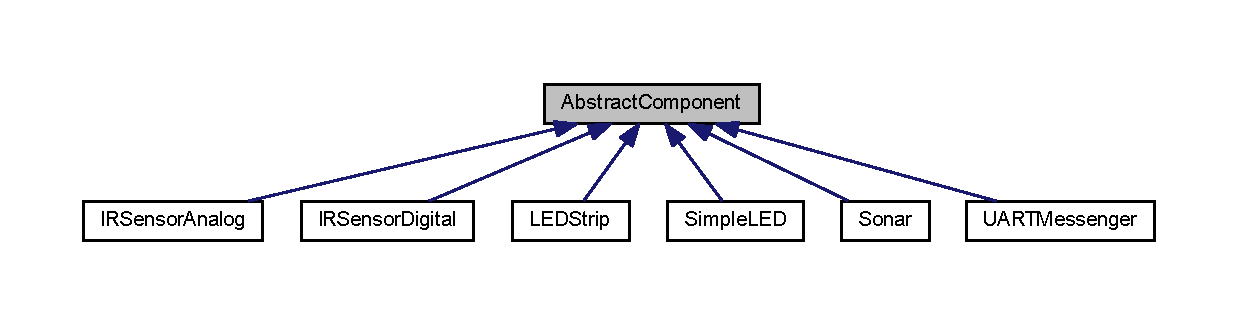
\includegraphics[width=350pt]{class_abstract_component__inherit__graph}
\end{center}
\end{figure}
\subsection*{Public Member Functions}
\begin{DoxyCompactItemize}
\item 
virtual void \hyperlink{class_abstract_component_af25a90b8ab213762221c3b358d9873f3}{update} ()=0
\item 
void \hyperlink{class_abstract_component_a58a59a9ea6c3b4c86fb3bf98ff1eaaef}{set\+Priority} (int p)
\begin{DoxyCompactList}\small\item\em Set priority to the component, used for updating order. \end{DoxyCompactList}\item 
int \hyperlink{class_abstract_component_ac0b440d1d642ff1292ec3c544d75a8f1}{get\+Priority} ()
\item 
bool \hyperlink{class_abstract_component_a0c2e458144111c5f599c66f168516abc}{operator$<$} (const \hyperlink{class_abstract_component}{Abstract\+Component} \&another) const
\begin{DoxyCompactList}\small\item\em Overloaded comparison operator \textquotesingle{}$<$\textquotesingle{}. \end{DoxyCompactList}\end{DoxyCompactItemize}
\subsection*{Protected Attributes}
\begin{DoxyCompactItemize}
\item 
int \hyperlink{class_abstract_component_a9c9c548149681b1a1dd935e66ed5dd11}{id}
\item 
int \hyperlink{class_abstract_component_aff57dfa5f31be093a06b55560e33fb95}{priority} = 0
\end{DoxyCompactItemize}
\subsection*{Static Protected Attributes}
\begin{DoxyCompactItemize}
\item 
static int \hyperlink{class_abstract_component_a99ce3e5fe7d73dac569b874c15fcaf0d}{s\+\_\+id} = 0
\begin{DoxyCompactList}\small\item\em The id for each component will be created in a sequence order staring with 1. \end{DoxyCompactList}\end{DoxyCompactItemize}


\subsection{Detailed Description}


Definition at line 8 of file Abstract\+Component.\+h.



\subsection{Member Function Documentation}
\mbox{\Hypertarget{class_abstract_component_ac0b440d1d642ff1292ec3c544d75a8f1}\label{class_abstract_component_ac0b440d1d642ff1292ec3c544d75a8f1}} 
\index{Abstract\+Component@{Abstract\+Component}!get\+Priority@{get\+Priority}}
\index{get\+Priority@{get\+Priority}!Abstract\+Component@{Abstract\+Component}}
\subsubsection{\texorpdfstring{get\+Priority()}{getPriority()}}
{\footnotesize\ttfamily int Abstract\+Component\+::get\+Priority (\begin{DoxyParamCaption}{ }\end{DoxyParamCaption})\hspace{0.3cm}{\ttfamily [inline]}}

\begin{DoxyReturn}{Returns}
priority of the component 
\end{DoxyReturn}


Definition at line 25 of file Abstract\+Component.\+h.


\begin{DoxyCode}
25                       \{
26         \textcolor{keywordflow}{return} \hyperlink{class_abstract_component_aff57dfa5f31be093a06b55560e33fb95}{priority};
27     \}
\end{DoxyCode}
Here is the call graph for this function\+:
\nopagebreak
\begin{figure}[H]
\begin{center}
\leavevmode
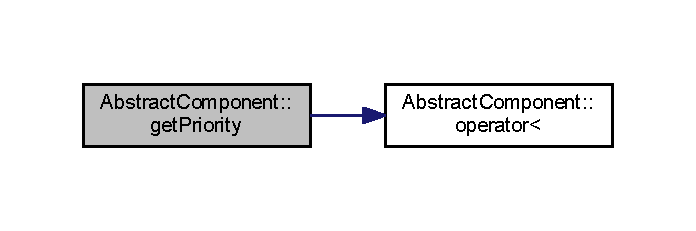
\includegraphics[width=334pt]{class_abstract_component_ac0b440d1d642ff1292ec3c544d75a8f1_cgraph}
\end{center}
\end{figure}
\mbox{\Hypertarget{class_abstract_component_a0c2e458144111c5f599c66f168516abc}\label{class_abstract_component_a0c2e458144111c5f599c66f168516abc}} 
\index{Abstract\+Component@{Abstract\+Component}!operator$<$@{operator$<$}}
\index{operator$<$@{operator$<$}!Abstract\+Component@{Abstract\+Component}}
\subsubsection{\texorpdfstring{operator$<$()}{operator<()}}
{\footnotesize\ttfamily bool Abstract\+Component\+::operator$<$ (\begin{DoxyParamCaption}\item[{const \hyperlink{class_abstract_component}{Abstract\+Component} \&}]{another }\end{DoxyParamCaption}) const}



Overloaded comparison operator \textquotesingle{}$<$\textquotesingle{}. 


\begin{DoxyParams}{Parameters}
{\em another} & component for comparison \\
\hline
\end{DoxyParams}
\begin{DoxyReturn}{Returns}
true if id is smaller then the id of another component 
\end{DoxyReturn}


Definition at line 8 of file Abstract\+Component.\+cpp.


\begin{DoxyCode}
8                                                                         \{
9     \textcolor{keywordflow}{return} \textcolor{keywordtype}{id} < another.\hyperlink{class_abstract_component_a9c9c548149681b1a1dd935e66ed5dd11}{id};
10 \}
\end{DoxyCode}
Here is the caller graph for this function\+:
\nopagebreak
\begin{figure}[H]
\begin{center}
\leavevmode
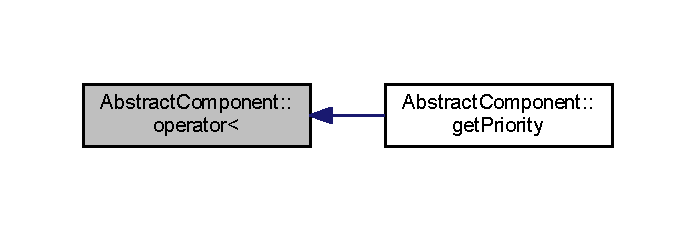
\includegraphics[width=334pt]{class_abstract_component_a0c2e458144111c5f599c66f168516abc_icgraph}
\end{center}
\end{figure}
\mbox{\Hypertarget{class_abstract_component_a58a59a9ea6c3b4c86fb3bf98ff1eaaef}\label{class_abstract_component_a58a59a9ea6c3b4c86fb3bf98ff1eaaef}} 
\index{Abstract\+Component@{Abstract\+Component}!set\+Priority@{set\+Priority}}
\index{set\+Priority@{set\+Priority}!Abstract\+Component@{Abstract\+Component}}
\subsubsection{\texorpdfstring{set\+Priority()}{setPriority()}}
{\footnotesize\ttfamily void Abstract\+Component\+::set\+Priority (\begin{DoxyParamCaption}\item[{int}]{p }\end{DoxyParamCaption})\hspace{0.3cm}{\ttfamily [inline]}}



Set priority to the component, used for updating order. 


\begin{DoxyParams}{Parameters}
{\em p} & priority \\
\hline
\end{DoxyParams}


Definition at line 18 of file Abstract\+Component.\+h.


\begin{DoxyCode}
18                             \{
19         \hyperlink{class_abstract_component_aff57dfa5f31be093a06b55560e33fb95}{priority} = p;
20     \}
\end{DoxyCode}
\mbox{\Hypertarget{class_abstract_component_af25a90b8ab213762221c3b358d9873f3}\label{class_abstract_component_af25a90b8ab213762221c3b358d9873f3}} 
\index{Abstract\+Component@{Abstract\+Component}!update@{update}}
\index{update@{update}!Abstract\+Component@{Abstract\+Component}}
\subsubsection{\texorpdfstring{update()}{update()}}
{\footnotesize\ttfamily virtual void Abstract\+Component\+::update (\begin{DoxyParamCaption}{ }\end{DoxyParamCaption})\hspace{0.3cm}{\ttfamily [pure virtual]}}



Implemented in \hyperlink{class_l_e_d_strip_abc57d90870bb0e9c0d05e7ba6ca76c95}{L\+E\+D\+Strip}, \hyperlink{class_i_r_sensor_analog_a919942de7c5fc3af5da9a2b32e31d328}{I\+R\+Sensor\+Analog}, \hyperlink{class_simple_l_e_d_a1642dc4aca42ad46e5663a39cdda005f}{Simple\+L\+ED}, \hyperlink{class_i_r_sensor_digital_a8d09a546a1f4b4c6533c324d98a146a9}{I\+R\+Sensor\+Digital}, \hyperlink{class_u_a_r_t_messenger_a7f2c3bdcf3a2b082e52815b97be37281}{U\+A\+R\+T\+Messenger}, and \hyperlink{class_sonar_aaf10dd734528b86b4dea3ab35c4ee4f4}{Sonar}.



\subsection{Member Data Documentation}
\mbox{\Hypertarget{class_abstract_component_a9c9c548149681b1a1dd935e66ed5dd11}\label{class_abstract_component_a9c9c548149681b1a1dd935e66ed5dd11}} 
\index{Abstract\+Component@{Abstract\+Component}!id@{id}}
\index{id@{id}!Abstract\+Component@{Abstract\+Component}}
\subsubsection{\texorpdfstring{id}{id}}
{\footnotesize\ttfamily int Abstract\+Component\+::id\hspace{0.3cm}{\ttfamily [protected]}}



Definition at line 39 of file Abstract\+Component.\+h.

\mbox{\Hypertarget{class_abstract_component_aff57dfa5f31be093a06b55560e33fb95}\label{class_abstract_component_aff57dfa5f31be093a06b55560e33fb95}} 
\index{Abstract\+Component@{Abstract\+Component}!priority@{priority}}
\index{priority@{priority}!Abstract\+Component@{Abstract\+Component}}
\subsubsection{\texorpdfstring{priority}{priority}}
{\footnotesize\ttfamily int Abstract\+Component\+::priority = 0\hspace{0.3cm}{\ttfamily [protected]}}



Definition at line 40 of file Abstract\+Component.\+h.

\mbox{\Hypertarget{class_abstract_component_a99ce3e5fe7d73dac569b874c15fcaf0d}\label{class_abstract_component_a99ce3e5fe7d73dac569b874c15fcaf0d}} 
\index{Abstract\+Component@{Abstract\+Component}!s\+\_\+id@{s\+\_\+id}}
\index{s\+\_\+id@{s\+\_\+id}!Abstract\+Component@{Abstract\+Component}}
\subsubsection{\texorpdfstring{s\+\_\+id}{s\_id}}
{\footnotesize\ttfamily int Abstract\+Component\+::s\+\_\+id = 0\hspace{0.3cm}{\ttfamily [static]}, {\ttfamily [protected]}}



The id for each component will be created in a sequence order staring with 1. 



Definition at line 38 of file Abstract\+Component.\+h.



The documentation for this class was generated from the following files\+:\begin{DoxyCompactItemize}
\item 
\hyperlink{_abstract_component_8h}{Abstract\+Component.\+h}\item 
\hyperlink{_abstract_component_8cpp}{Abstract\+Component.\+cpp}\end{DoxyCompactItemize}

\hypertarget{class_i_r_q_lock}{}\section{I\+R\+Q\+Lock Class Reference}
\label{class_i_r_q_lock}\index{I\+R\+Q\+Lock@{I\+R\+Q\+Lock}}


{\ttfamily \#include $<$I\+R\+Q\+Lock.\+h$>$}



\subsection{Detailed Description}
In some cases, we want to ensure a section of code is not interrupted. For example, you might be talking to a peripheral where the whole transaction must happen in one go, and an interrupt could cause the operation to fail. So we use the constructor and deconstructor of I\+RQ Lock. 

The documentation for this class was generated from the following file\+:\begin{DoxyCompactItemize}
\item 
I\+R\+Q\+Lock.\+h\end{DoxyCompactItemize}

\hypertarget{class_i_r_sensor_analog}{}\section{I\+R\+Sensor\+Analog Class Reference}
\label{class_i_r_sensor_analog}\index{I\+R\+Sensor\+Analog@{I\+R\+Sensor\+Analog}}


{\ttfamily \#include $<$I\+R\+Sensor\+Analog.\+h$>$}

Inheritance diagram for I\+R\+Sensor\+Analog\+:\begin{figure}[H]
\begin{center}
\leavevmode
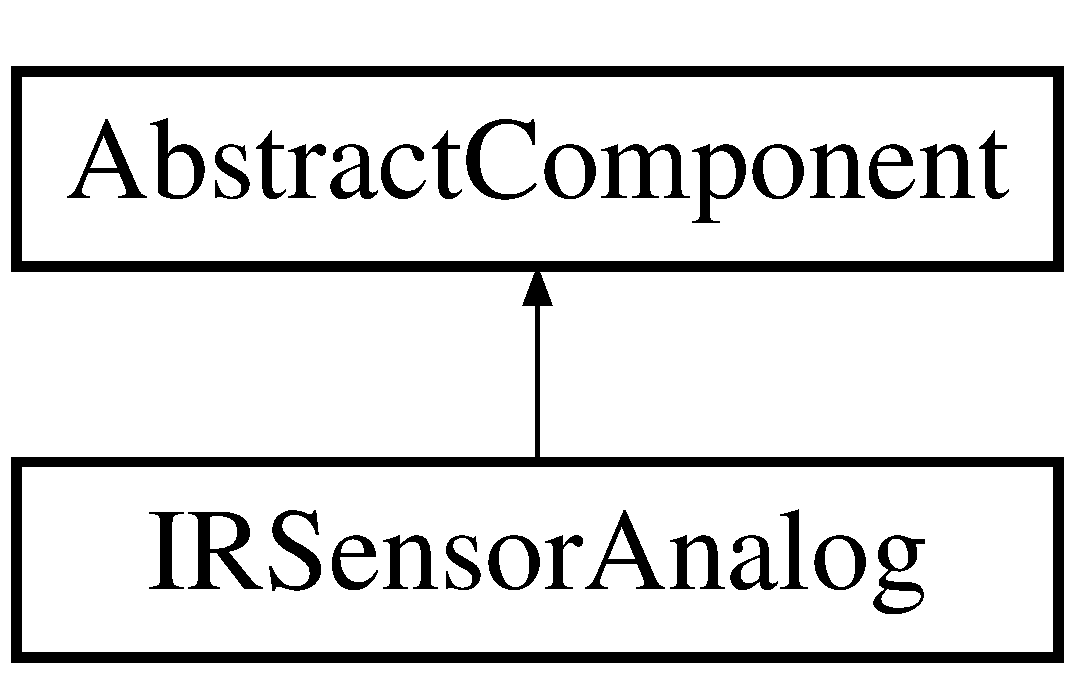
\includegraphics[height=2.000000cm]{class_i_r_sensor_analog}
\end{center}
\end{figure}
\subsection*{Public Member Functions}
\begin{DoxyCompactItemize}
\item 
\hyperlink{class_i_r_sensor_analog_af27166832035783b3df081014c4dfb9d}{I\+R\+Sensor\+Analog} (\hyperlink{class_u_a_r_t_messenger}{U\+A\+R\+T\+Messenger} $\ast$const uart\+Msngr, Pin\+Name data\+Pin, std\+::vector$<$ std\+::vector$<$ int $>$ $>$ lookup\+Table)
\item 
float \hyperlink{class_i_r_sensor_analog_aa6642b85ec1018980e216eab0dfd27f2}{get\+Range} ()
\item 
virtual void \hyperlink{class_i_r_sensor_analog_a919942de7c5fc3af5da9a2b32e31d328}{update} ()
\end{DoxyCompactItemize}
\subsection*{Additional Inherited Members}


\subsection{Constructor \& Destructor Documentation}
\mbox{\Hypertarget{class_i_r_sensor_analog_af27166832035783b3df081014c4dfb9d}\label{class_i_r_sensor_analog_af27166832035783b3df081014c4dfb9d}} 
\index{I\+R\+Sensor\+Analog@{I\+R\+Sensor\+Analog}!I\+R\+Sensor\+Analog@{I\+R\+Sensor\+Analog}}
\index{I\+R\+Sensor\+Analog@{I\+R\+Sensor\+Analog}!I\+R\+Sensor\+Analog@{I\+R\+Sensor\+Analog}}
\subsubsection{\texorpdfstring{I\+R\+Sensor\+Analog()}{IRSensorAnalog()}}
{\footnotesize\ttfamily I\+R\+Sensor\+Analog\+::\+I\+R\+Sensor\+Analog (\begin{DoxyParamCaption}\item[{\hyperlink{class_u_a_r_t_messenger}{U\+A\+R\+T\+Messenger} $\ast$const}]{uart\+Msngr,  }\item[{Pin\+Name}]{pin,  }\item[{std\+::vector$<$ std\+::vector$<$ int $>$ $>$}]{lookup\+Table }\end{DoxyParamCaption})}


\begin{DoxyParams}{Parameters}
{\em uart\+Msngr} & \hyperlink{class_u_a_r_t_messenger}{U\+A\+R\+T\+Messenger} object for communicating with Paparazzi \\
\hline
{\em data\+Pin} & -\/ pin on board, where data pin of IR sensor is connected \\
\hline
{\em lookup\+Table} & -\/ two-\/dimensional array, describing relation between sensor output and distance, set in millimeters\\
\hline
\end{DoxyParams}
Constructor for analog I\+R\+Sensor 

\subsection{Member Function Documentation}
\mbox{\Hypertarget{class_i_r_sensor_analog_aa6642b85ec1018980e216eab0dfd27f2}\label{class_i_r_sensor_analog_aa6642b85ec1018980e216eab0dfd27f2}} 
\index{I\+R\+Sensor\+Analog@{I\+R\+Sensor\+Analog}!get\+Range@{get\+Range}}
\index{get\+Range@{get\+Range}!I\+R\+Sensor\+Analog@{I\+R\+Sensor\+Analog}}
\subsubsection{\texorpdfstring{get\+Range()}{getRange()}}
{\footnotesize\ttfamily float I\+R\+Sensor\+Analog\+::get\+Range (\begin{DoxyParamCaption}{ }\end{DoxyParamCaption})}

\begin{DoxyReturn}{Returns}
-\/ range of sensor in meters 
\end{DoxyReturn}
\mbox{\Hypertarget{class_i_r_sensor_analog_a919942de7c5fc3af5da9a2b32e31d328}\label{class_i_r_sensor_analog_a919942de7c5fc3af5da9a2b32e31d328}} 
\index{I\+R\+Sensor\+Analog@{I\+R\+Sensor\+Analog}!update@{update}}
\index{update@{update}!I\+R\+Sensor\+Analog@{I\+R\+Sensor\+Analog}}
\subsubsection{\texorpdfstring{update()}{update()}}
{\footnotesize\ttfamily void I\+R\+Sensor\+Analog\+::update (\begin{DoxyParamCaption}{ }\end{DoxyParamCaption})\hspace{0.3cm}{\ttfamily [virtual]}}

Read the sensor value and product with the reference voltage. We can get range from to\+Range() function. Submessage is struct where we get type of the sensor = I\+R\+A\+N\+A\+L\+OG, id of the sensor, data, length of the range size. Uart\+Messenger appends submessage which is in \hyperlink{class_u_a_r_t_messenger}{U\+A\+R\+T\+Messenger}. 

Implements \hyperlink{class_abstract_component_af25a90b8ab213762221c3b358d9873f3}{Abstract\+Component}.



The documentation for this class was generated from the following files\+:\begin{DoxyCompactItemize}
\item 
\hyperlink{_i_r_sensor_analog_8h}{I\+R\+Sensor\+Analog.\+h}\item 
\hyperlink{_i_r_sensor_analog_8cpp}{I\+R\+Sensor\+Analog.\+cpp}\end{DoxyCompactItemize}

\hypertarget{class_i_r_sensor_digital}{}\section{I\+R\+Sensor\+Digital Class Reference}
\label{class_i_r_sensor_digital}\index{I\+R\+Sensor\+Digital@{I\+R\+Sensor\+Digital}}
Inheritance diagram for I\+R\+Sensor\+Digital\+:\begin{figure}[H]
\begin{center}
\leavevmode
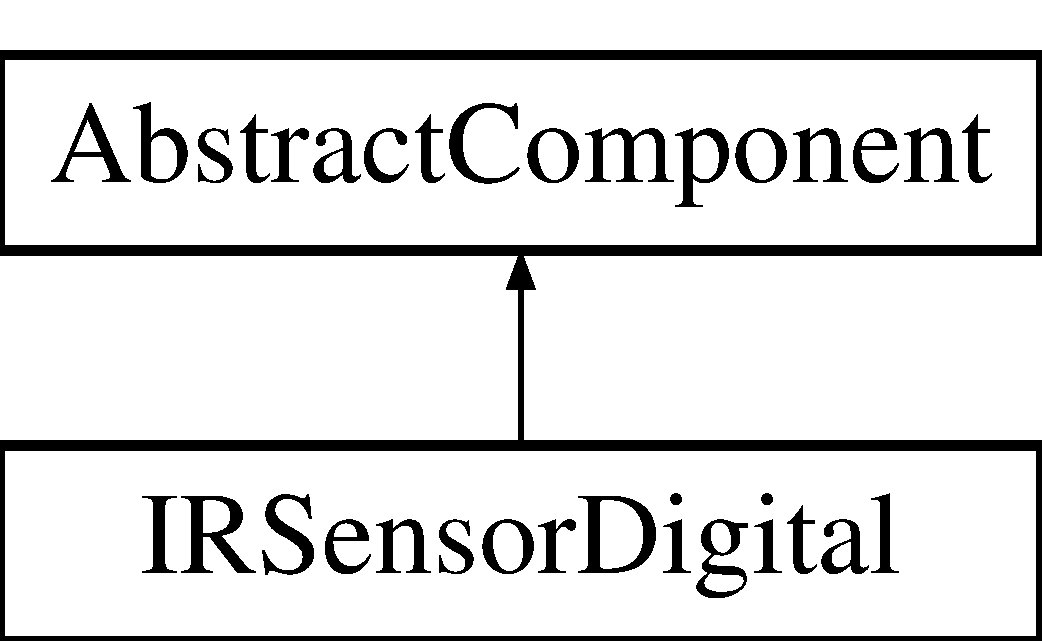
\includegraphics[height=2.000000cm]{class_i_r_sensor_digital}
\end{center}
\end{figure}
\subsection*{Public Member Functions}
\begin{DoxyCompactItemize}
\item 
\hyperlink{class_i_r_sensor_digital_a43d7d836d07616260611d3cef709dff1}{I\+R\+Sensor\+Digital} (\hyperlink{class_u_a_r_t_messenger}{U\+A\+R\+T\+Messenger} $\ast$const uart\+Msngr, Pin\+Name data\+Pin, float detection\+Range)
\item 
bool \hyperlink{class_i_r_sensor_digital_a749b91dae3e83900f6de49fcc908470d}{is\+In\+Range} ()
\item 
virtual void \hyperlink{class_i_r_sensor_digital_a8d09a546a1f4b4c6533c324d98a146a9}{update} ()
\end{DoxyCompactItemize}
\subsection*{Additional Inherited Members}


\subsection{Constructor \& Destructor Documentation}
\mbox{\Hypertarget{class_i_r_sensor_digital_a43d7d836d07616260611d3cef709dff1}\label{class_i_r_sensor_digital_a43d7d836d07616260611d3cef709dff1}} 
\index{I\+R\+Sensor\+Digital@{I\+R\+Sensor\+Digital}!I\+R\+Sensor\+Digital@{I\+R\+Sensor\+Digital}}
\index{I\+R\+Sensor\+Digital@{I\+R\+Sensor\+Digital}!I\+R\+Sensor\+Digital@{I\+R\+Sensor\+Digital}}
\subsubsection{\texorpdfstring{I\+R\+Sensor\+Digital()}{IRSensorDigital()}}
{\footnotesize\ttfamily I\+R\+Sensor\+Digital\+::\+I\+R\+Sensor\+Digital (\begin{DoxyParamCaption}\item[{\hyperlink{class_u_a_r_t_messenger}{U\+A\+R\+T\+Messenger} $\ast$const}]{uart\+Msngr,  }\item[{Pin\+Name}]{data\+Pin,  }\item[{float}]{detection\+Range }\end{DoxyParamCaption})}


\begin{DoxyParams}{Parameters}
{\em data\+Pin} & -\/ pin on board, where data pin of IR sensor is connected \\
\hline
{\em detection\+Range} & -\/ distance of detection for this sensor \\
\hline
\end{DoxyParams}


\subsection{Member Function Documentation}
\mbox{\Hypertarget{class_i_r_sensor_digital_a749b91dae3e83900f6de49fcc908470d}\label{class_i_r_sensor_digital_a749b91dae3e83900f6de49fcc908470d}} 
\index{I\+R\+Sensor\+Digital@{I\+R\+Sensor\+Digital}!is\+In\+Range@{is\+In\+Range}}
\index{is\+In\+Range@{is\+In\+Range}!I\+R\+Sensor\+Digital@{I\+R\+Sensor\+Digital}}
\subsubsection{\texorpdfstring{is\+In\+Range()}{isInRange()}}
{\footnotesize\ttfamily bool I\+R\+Sensor\+Digital\+::is\+In\+Range (\begin{DoxyParamCaption}{ }\end{DoxyParamCaption})}

\begin{DoxyReturn}{Returns}
true if sensor is in range 
\end{DoxyReturn}
\mbox{\Hypertarget{class_i_r_sensor_digital_a8d09a546a1f4b4c6533c324d98a146a9}\label{class_i_r_sensor_digital_a8d09a546a1f4b4c6533c324d98a146a9}} 
\index{I\+R\+Sensor\+Digital@{I\+R\+Sensor\+Digital}!update@{update}}
\index{update@{update}!I\+R\+Sensor\+Digital@{I\+R\+Sensor\+Digital}}
\subsubsection{\texorpdfstring{update()}{update()}}
{\footnotesize\ttfamily void I\+R\+Sensor\+Digital\+::update (\begin{DoxyParamCaption}{ }\end{DoxyParamCaption})\hspace{0.3cm}{\ttfamily [virtual]}}

If the value is less than the detection\+Range then it will return the true value. \hyperlink{struct_sub_message}{Sub\+Message} type is I\+R\+D\+I\+G\+I\+T\+AL, Id of the sensor. reinterpret\+\_\+cast is that submessage.\+data will be converted into boolean. Length is size of in\+Range. Appends the message to uart list. 

Implements \hyperlink{class_abstract_component}{Abstract\+Component}.



The documentation for this class was generated from the following files\+:\begin{DoxyCompactItemize}
\item 
I\+R\+Sensor\+Digital.\+h\item 
I\+R\+Sensor\+Digital.\+cpp\end{DoxyCompactItemize}

\hypertarget{class_l_e_d_strip}{}\section{L\+E\+D\+Strip Class Reference}
\label{class_l_e_d_strip}\index{L\+E\+D\+Strip@{L\+E\+D\+Strip}}
Inheritance diagram for L\+E\+D\+Strip\+:\begin{figure}[H]
\begin{center}
\leavevmode
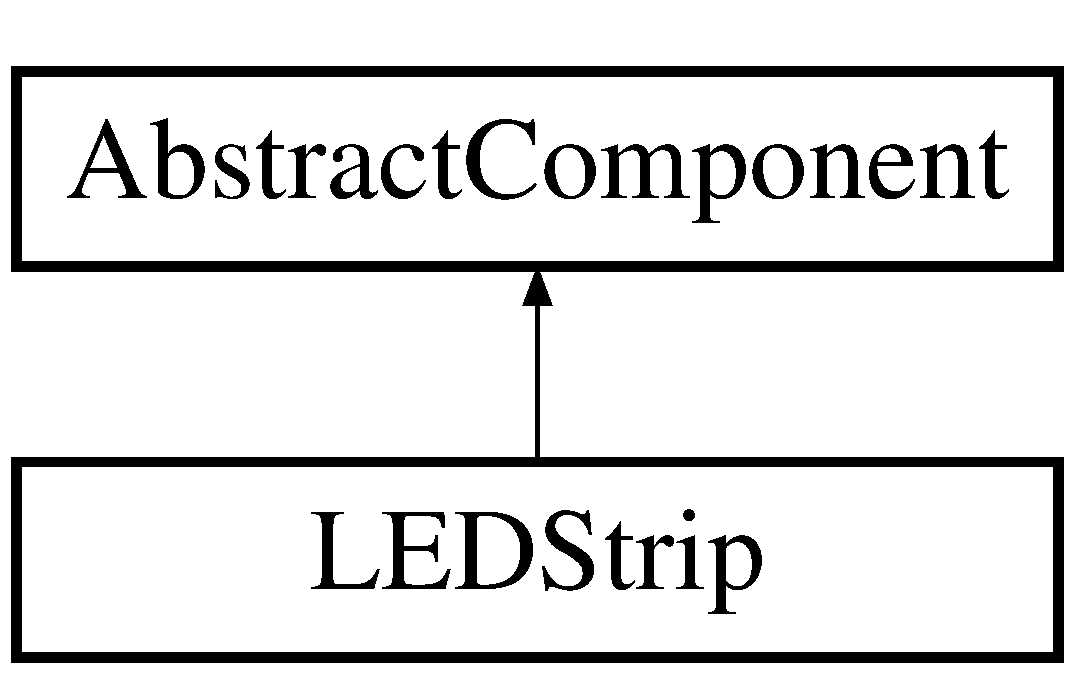
\includegraphics[height=2.000000cm]{class_l_e_d_strip}
\end{center}
\end{figure}
\subsection*{Public Member Functions}
\begin{DoxyCompactItemize}
\item 
\hyperlink{class_l_e_d_strip_a746e420e05c5d6c45eb2f74eaf5928fc}{L\+E\+D\+Strip} (\hyperlink{class_u_a_r_t_messenger}{U\+A\+R\+T\+Messenger} $\ast$const uart\+Msngr, Pin\+Name pin, int size, int zero\+High, int zero\+Low, int one\+High, int one\+Low)
\item 
void \hyperlink{class_l_e_d_strip_abf199367f3caaf9730262c4e7bef6bc1}{set\+Mode} (uint8\+\_\+t mode)
\item 
void \hyperlink{class_l_e_d_strip_a310b381acdd83a01ddb6e2debebbbc7c}{set\+Color} (unsigned int color)
\item 
void \hyperlink{class_l_e_d_strip_a1f9d9c2784c9ad893163f7f17e603ce7}{set\+Color} (unsigned int color, uint8\+\_\+t led=0)
\item 
virtual void \hyperlink{class_l_e_d_strip_abc57d90870bb0e9c0d05e7ba6ca76c95}{update} ()
\item 
virtual void \hyperlink{class_l_e_d_strip_af9708cc14c0e3f75e5b3c268b398f436}{on\+Paparazzi\+Msg} (\hyperlink{struct_sub_message}{Sub\+Message} $\ast$msg)
\end{DoxyCompactItemize}
\subsection*{Additional Inherited Members}


\subsection{Constructor \& Destructor Documentation}
\mbox{\Hypertarget{class_l_e_d_strip_a746e420e05c5d6c45eb2f74eaf5928fc}\label{class_l_e_d_strip_a746e420e05c5d6c45eb2f74eaf5928fc}} 
\index{L\+E\+D\+Strip@{L\+E\+D\+Strip}!L\+E\+D\+Strip@{L\+E\+D\+Strip}}
\index{L\+E\+D\+Strip@{L\+E\+D\+Strip}!L\+E\+D\+Strip@{L\+E\+D\+Strip}}
\subsubsection{\texorpdfstring{L\+E\+D\+Strip()}{LEDStrip()}}
{\footnotesize\ttfamily L\+E\+D\+Strip\+::\+L\+E\+D\+Strip (\begin{DoxyParamCaption}\item[{\hyperlink{class_u_a_r_t_messenger}{U\+A\+R\+T\+Messenger} $\ast$const}]{uart\+Msngr,  }\item[{Pin\+Name}]{pin,  }\item[{int}]{size,  }\item[{int}]{zero\+High,  }\item[{int}]{zero\+Low,  }\item[{int}]{one\+High,  }\item[{int}]{one\+Low }\end{DoxyParamCaption})}


\begin{DoxyParams}{Parameters}
{\em uart\+Msngr} & \hyperlink{class_u_a_r_t_messenger}{U\+A\+R\+T\+Messenger} object for communicating with Paparazzi \\
\hline
{\em pin} & Output pin. Connect to \char`\"{}\+Din\char`\"{} on the first \hyperlink{class_w_s2812}{W\+S2812} in the strip \\
\hline
{\em size} & Number of L\+E\+Ds in your strip \\
\hline
{\em zero\+High} & How many N\+O\+Ps to insert to ensure T\+OH is properly generated. See library description for more information. \\
\hline
{\em zero\+Low} & How many N\+O\+Ps to insert to ensure T\+OL is properly generated. See library description for more information. \\
\hline
{\em one\+High} & How many N\+O\+Ps to insert to ensure T1H is properly generated. See library description for more information. \\
\hline
{\em one\+Low} & How many N\+O\+Ps to insert to ensure T1L is properly generated. See library description for more information.\\
\hline
\end{DoxyParams}
Constructor for creating a new L\+ED Strip. 

\subsection{Member Function Documentation}
\mbox{\Hypertarget{class_l_e_d_strip_af9708cc14c0e3f75e5b3c268b398f436}\label{class_l_e_d_strip_af9708cc14c0e3f75e5b3c268b398f436}} 
\index{L\+E\+D\+Strip@{L\+E\+D\+Strip}!on\+Paparazzi\+Msg@{on\+Paparazzi\+Msg}}
\index{on\+Paparazzi\+Msg@{on\+Paparazzi\+Msg}!L\+E\+D\+Strip@{L\+E\+D\+Strip}}
\subsubsection{\texorpdfstring{on\+Paparazzi\+Msg()}{onPaparazziMsg()}}
{\footnotesize\ttfamily void L\+E\+D\+Strip\+::on\+Paparazzi\+Msg (\begin{DoxyParamCaption}\item[{\hyperlink{struct_sub_message}{Sub\+Message} $\ast$}]{msg }\end{DoxyParamCaption})\hspace{0.3cm}{\ttfamily [virtual]}}


\begin{DoxyParams}{Parameters}
{\em msg} & message struct from Paparazzi\\
\hline
\end{DoxyParams}
Reaction on the message from Paparazzi. Expected message structure\+: type (1 byte), id (1 byte), length (1 byte), data (length byte) Datastructure\+: led id (1 byte), red channel (1 byte), green channel (1 byte), blue channel (1 byte) \hyperlink{struct_sub_message}{Sub\+Message} came from Paparazzi \mbox{\Hypertarget{class_l_e_d_strip_a310b381acdd83a01ddb6e2debebbbc7c}\label{class_l_e_d_strip_a310b381acdd83a01ddb6e2debebbbc7c}} 
\index{L\+E\+D\+Strip@{L\+E\+D\+Strip}!set\+Color@{set\+Color}}
\index{set\+Color@{set\+Color}!L\+E\+D\+Strip@{L\+E\+D\+Strip}}
\subsubsection{\texorpdfstring{set\+Color()}{setColor()}\hspace{0.1cm}{\footnotesize\ttfamily [1/2]}}
{\footnotesize\ttfamily void L\+E\+D\+Strip\+::set\+Color (\begin{DoxyParamCaption}\item[{unsigned int}]{color }\end{DoxyParamCaption})}


\begin{DoxyParams}{Parameters}
{\em color} & color in R\+GB format, e.\+g. 0x00\+F\+F00\\
\hline
\end{DoxyParams}
Set color to L\+ED Strip. \mbox{\Hypertarget{class_l_e_d_strip_a1f9d9c2784c9ad893163f7f17e603ce7}\label{class_l_e_d_strip_a1f9d9c2784c9ad893163f7f17e603ce7}} 
\index{L\+E\+D\+Strip@{L\+E\+D\+Strip}!set\+Color@{set\+Color}}
\index{set\+Color@{set\+Color}!L\+E\+D\+Strip@{L\+E\+D\+Strip}}
\subsubsection{\texorpdfstring{set\+Color()}{setColor()}\hspace{0.1cm}{\footnotesize\ttfamily [2/2]}}
{\footnotesize\ttfamily void L\+E\+D\+Strip\+::set\+Color (\begin{DoxyParamCaption}\item[{unsigned int}]{color,  }\item[{uint8\+\_\+t}]{led = {\ttfamily 0} }\end{DoxyParamCaption})}


\begin{DoxyParams}{Parameters}
{\em color} & color in R\+GB format, e.\+g. 0x00\+F\+F00 \\
\hline
{\em led} & id of the L\+ED to use\\
\hline
\end{DoxyParams}
Set color to only one L\+ED \mbox{\Hypertarget{class_l_e_d_strip_abf199367f3caaf9730262c4e7bef6bc1}\label{class_l_e_d_strip_abf199367f3caaf9730262c4e7bef6bc1}} 
\index{L\+E\+D\+Strip@{L\+E\+D\+Strip}!set\+Mode@{set\+Mode}}
\index{set\+Mode@{set\+Mode}!L\+E\+D\+Strip@{L\+E\+D\+Strip}}
\subsubsection{\texorpdfstring{set\+Mode()}{setMode()}}
{\footnotesize\ttfamily void L\+E\+D\+Strip\+::set\+Mode (\begin{DoxyParamCaption}\item[{uint8\+\_\+t}]{mode }\end{DoxyParamCaption})}


\begin{DoxyParams}{Parameters}
{\em mode} & one of predifined modes\\
\hline
\end{DoxyParams}
Set L\+ED Strip to manual control instead of getting control action from paparazzi, which is set by default. \mbox{\Hypertarget{class_l_e_d_strip_abc57d90870bb0e9c0d05e7ba6ca76c95}\label{class_l_e_d_strip_abc57d90870bb0e9c0d05e7ba6ca76c95}} 
\index{L\+E\+D\+Strip@{L\+E\+D\+Strip}!update@{update}}
\index{update@{update}!L\+E\+D\+Strip@{L\+E\+D\+Strip}}
\subsubsection{\texorpdfstring{update()}{update()}}
{\footnotesize\ttfamily void L\+E\+D\+Strip\+::update (\begin{DoxyParamCaption}{ }\end{DoxyParamCaption})\hspace{0.3cm}{\ttfamily [virtual]}}

The update function will be to the L\+E\+Dstrip when the control from paparazzi is received and check the message from paparrazi with respect to id. Then check if the paparazzi message received is not null then go to the method on\+Paparazzi\+Msg to recieve paparazzi message. set write offset passing parameters. while giving the the submessage provide the L\+ED strip Id and append message to the uart messenger 

Implements \hyperlink{class_abstract_component}{Abstract\+Component}.



The documentation for this class was generated from the following files\+:\begin{DoxyCompactItemize}
\item 
L\+E\+D\+Strip.\+h\item 
L\+E\+D\+Strip.\+cpp\end{DoxyCompactItemize}

\hypertarget{class_pixel_array}{}\section{Pixel\+Array Class Reference}
\label{class_pixel_array}\index{Pixel\+Array@{Pixel\+Array}}


Library for the \hyperlink{class_w_s2812}{W\+S2812} R\+GB L\+ED with integrated controller.  




{\ttfamily \#include $<$Pixel\+Array.\+h$>$}

\subsection*{Public Member Functions}
\begin{DoxyCompactItemize}
\item 
\hyperlink{class_pixel_array_a86359f5eda90e0d12e3aa2c102ade21d}{Pixel\+Array} (int)
\begin{DoxyCompactList}\small\item\em Creates an instance of the class. \end{DoxyCompactList}\item 
\hyperlink{class_pixel_array_a9f4d10fcbd08290dfdecafb2ed4ad687}{$\sim$\+Pixel\+Array} ()
\item 
int $\ast$ \hyperlink{class_pixel_array_a987f1dc053a5cf25d78d5cfe037088d3}{get\+Buf} ()
\item 
void \hyperlink{class_pixel_array_a5f560dcef3d1582614858969b20da89d}{Set\+All} (unsigned int)
\item 
void \hyperlink{class_pixel_array_a9433e281c3cc0e4f8bbf23e127d8ad2c}{Set\+AllI} (unsigned char)
\item 
void \hyperlink{class_pixel_array_a9ddfdd1a01a9877e4bfcf5a462412fd2}{Set\+AllR} (unsigned char)
\item 
void \hyperlink{class_pixel_array_a88f25ee1b266e2dc0ef7ae90ff4bd12d}{Set\+AllG} (unsigned char)
\item 
void \hyperlink{class_pixel_array_a3b17271fdc21503236ca6ca8e37d501b}{Set\+AllB} (unsigned char)
\item 
void \hyperlink{class_pixel_array_afcfe32b74beeced27f928f42131d77c1}{Set} (int, unsigned int)
\item 
void \hyperlink{class_pixel_array_afbfac74c674f63d793d85141d3a3b046}{SetI} (int, unsigned char)
\item 
void \hyperlink{class_pixel_array_abd4253e7c76f3775f31e09dfe318e3a5}{SetR} (int, unsigned char)
\item 
void \hyperlink{class_pixel_array_a60ea8084ec95df0d51f46c9b0ff308d5}{SetG} (int, unsigned char)
\item 
void \hyperlink{class_pixel_array_a560a654c59614fd5a6c17adb10083a78}{SetB} (int, unsigned char)
\end{DoxyCompactItemize}
\subsection*{Private Member Functions}
\begin{DoxyCompactItemize}
\item 
void \hyperlink{class_pixel_array_a42c6681bf771332826ecc9ad2a8cea02}{\+\_\+\+\_\+set\+\_\+pixel\+\_\+component} (int index, int channel, int value)
\item 
void \hyperlink{class_pixel_array_a4b1a6582bc3bab1f67aebd1f97a5595d}{\+\_\+\+\_\+set\+\_\+pixel} (int index, int value)
\end{DoxyCompactItemize}
\subsection*{Private Attributes}
\begin{DoxyCompactItemize}
\item 
int $\ast$ \hyperlink{class_pixel_array_ab0109a336e69a9942b2723e43ee715d7}{pbuf}
\item 
int \hyperlink{class_pixel_array_aca29e70f9b643bff3733ab2e694439a1}{pbufsize}
\end{DoxyCompactItemize}


\subsection{Detailed Description}
Library for the \hyperlink{class_w_s2812}{W\+S2812} R\+GB L\+ED with integrated controller. 

\hyperlink{class_pixel_array}{Pixel\+Array} 

Definition at line 10 of file Pixel\+Array.\+h.



\subsection{Constructor \& Destructor Documentation}
\mbox{\Hypertarget{class_pixel_array_a86359f5eda90e0d12e3aa2c102ade21d}\label{class_pixel_array_a86359f5eda90e0d12e3aa2c102ade21d}} 
\index{Pixel\+Array@{Pixel\+Array}!Pixel\+Array@{Pixel\+Array}}
\index{Pixel\+Array@{Pixel\+Array}!Pixel\+Array@{Pixel\+Array}}
\subsubsection{\texorpdfstring{Pixel\+Array()}{PixelArray()}}
{\footnotesize\ttfamily Pixel\+Array\+::\+Pixel\+Array (\begin{DoxyParamCaption}\item[{int}]{size }\end{DoxyParamCaption})}



Creates an instance of the class. 

Library for the \hyperlink{class_w_s2812}{W\+S2812} R\+GB L\+ED with integrated controller.

Pixel Array 

Definition at line 8 of file Pixel\+Array.\+cpp.


\begin{DoxyCode}
9 \{
10     \hyperlink{class_pixel_array_aca29e70f9b643bff3733ab2e694439a1}{pbufsize} = size;
11     \hyperlink{class_pixel_array_ab0109a336e69a9942b2723e43ee715d7}{pbuf} = \textcolor{keyword}{new} \textcolor{keywordtype}{int}[\hyperlink{class_pixel_array_aca29e70f9b643bff3733ab2e694439a1}{pbufsize}];
12     \hyperlink{class_pixel_array_a5f560dcef3d1582614858969b20da89d}{SetAll}(0x0); \textcolor{comment}{// initialise memory to zeros}
13 
14 \}
\end{DoxyCode}
Here is the call graph for this function\+:\nopagebreak
\begin{figure}[H]
\begin{center}
\leavevmode
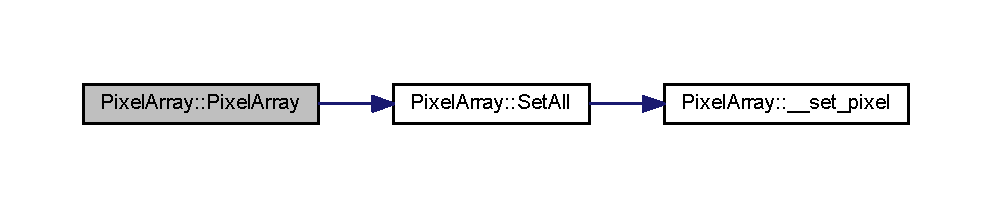
\includegraphics[width=350pt]{class_pixel_array_a86359f5eda90e0d12e3aa2c102ade21d_cgraph}
\end{center}
\end{figure}
\mbox{\Hypertarget{class_pixel_array_a9f4d10fcbd08290dfdecafb2ed4ad687}\label{class_pixel_array_a9f4d10fcbd08290dfdecafb2ed4ad687}} 
\index{Pixel\+Array@{Pixel\+Array}!````~Pixel\+Array@{$\sim$\+Pixel\+Array}}
\index{````~Pixel\+Array@{$\sim$\+Pixel\+Array}!Pixel\+Array@{Pixel\+Array}}
\subsubsection{\texorpdfstring{$\sim$\+Pixel\+Array()}{~PixelArray()}}
{\footnotesize\ttfamily Pixel\+Array\+::$\sim$\+Pixel\+Array (\begin{DoxyParamCaption}{ }\end{DoxyParamCaption})}

Destroys instance. 

Definition at line 20 of file Pixel\+Array.\+cpp.


\begin{DoxyCode}
21 \{
22     \textcolor{keyword}{delete}[] \hyperlink{class_pixel_array_ab0109a336e69a9942b2723e43ee715d7}{pbuf};
23 \}
\end{DoxyCode}


\subsection{Member Function Documentation}
\mbox{\Hypertarget{class_pixel_array_a4b1a6582bc3bab1f67aebd1f97a5595d}\label{class_pixel_array_a4b1a6582bc3bab1f67aebd1f97a5595d}} 
\index{Pixel\+Array@{Pixel\+Array}!\+\_\+\+\_\+set\+\_\+pixel@{\+\_\+\+\_\+set\+\_\+pixel}}
\index{\+\_\+\+\_\+set\+\_\+pixel@{\+\_\+\+\_\+set\+\_\+pixel}!Pixel\+Array@{Pixel\+Array}}
\subsubsection{\texorpdfstring{\+\_\+\+\_\+set\+\_\+pixel()}{\_\_set\_pixel()}}
{\footnotesize\ttfamily void Pixel\+Array\+::\+\_\+\+\_\+set\+\_\+pixel (\begin{DoxyParamCaption}\item[{int}]{index,  }\item[{int}]{value }\end{DoxyParamCaption})\hspace{0.3cm}{\ttfamily [private]}}



Definition at line 136 of file Pixel\+Array.\+cpp.


\begin{DoxyCode}
137 \{
138     \textcolor{comment}{// AND with 0x00 shifted to the right location to clear the bits}
139     \hyperlink{class_pixel_array_ab0109a336e69a9942b2723e43ee715d7}{pbuf}[index] = value;
140 \}
\end{DoxyCode}
Here is the caller graph for this function\+:\nopagebreak
\begin{figure}[H]
\begin{center}
\leavevmode
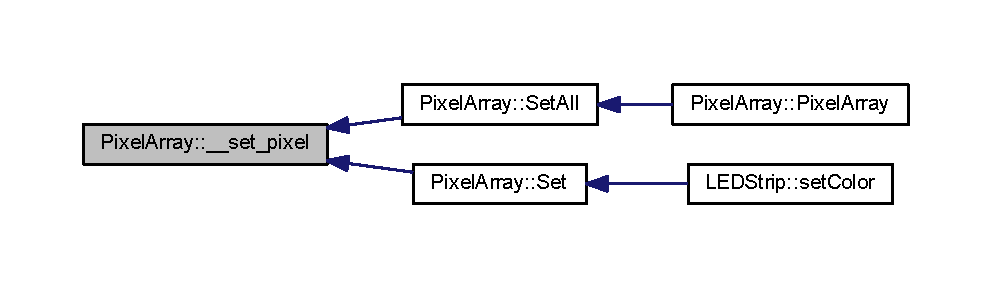
\includegraphics[width=350pt]{class_pixel_array_a4b1a6582bc3bab1f67aebd1f97a5595d_icgraph}
\end{center}
\end{figure}
\mbox{\Hypertarget{class_pixel_array_a42c6681bf771332826ecc9ad2a8cea02}\label{class_pixel_array_a42c6681bf771332826ecc9ad2a8cea02}} 
\index{Pixel\+Array@{Pixel\+Array}!\+\_\+\+\_\+set\+\_\+pixel\+\_\+component@{\+\_\+\+\_\+set\+\_\+pixel\+\_\+component}}
\index{\+\_\+\+\_\+set\+\_\+pixel\+\_\+component@{\+\_\+\+\_\+set\+\_\+pixel\+\_\+component}!Pixel\+Array@{Pixel\+Array}}
\subsubsection{\texorpdfstring{\+\_\+\+\_\+set\+\_\+pixel\+\_\+component()}{\_\_set\_pixel\_component()}}
{\footnotesize\ttfamily void Pixel\+Array\+::\+\_\+\+\_\+set\+\_\+pixel\+\_\+component (\begin{DoxyParamCaption}\item[{int}]{index,  }\item[{int}]{channel,  }\item[{int}]{value }\end{DoxyParamCaption})\hspace{0.3cm}{\ttfamily [private]}}



Definition at line 124 of file Pixel\+Array.\+cpp.


\begin{DoxyCode}
125 \{
126 
127     \textcolor{comment}{// AND with 0x00 shifted to the right location to clear the bits}
128     \hyperlink{class_pixel_array_ab0109a336e69a9942b2723e43ee715d7}{pbuf}[index] &= ~(0xFF << (8 * channel));
129 
130     \textcolor{comment}{// Set the bits with an OR}
131     \hyperlink{class_pixel_array_ab0109a336e69a9942b2723e43ee715d7}{pbuf}[index] |= (value << (8 * channel));
132 \}
\end{DoxyCode}
Here is the caller graph for this function\+:\nopagebreak
\begin{figure}[H]
\begin{center}
\leavevmode
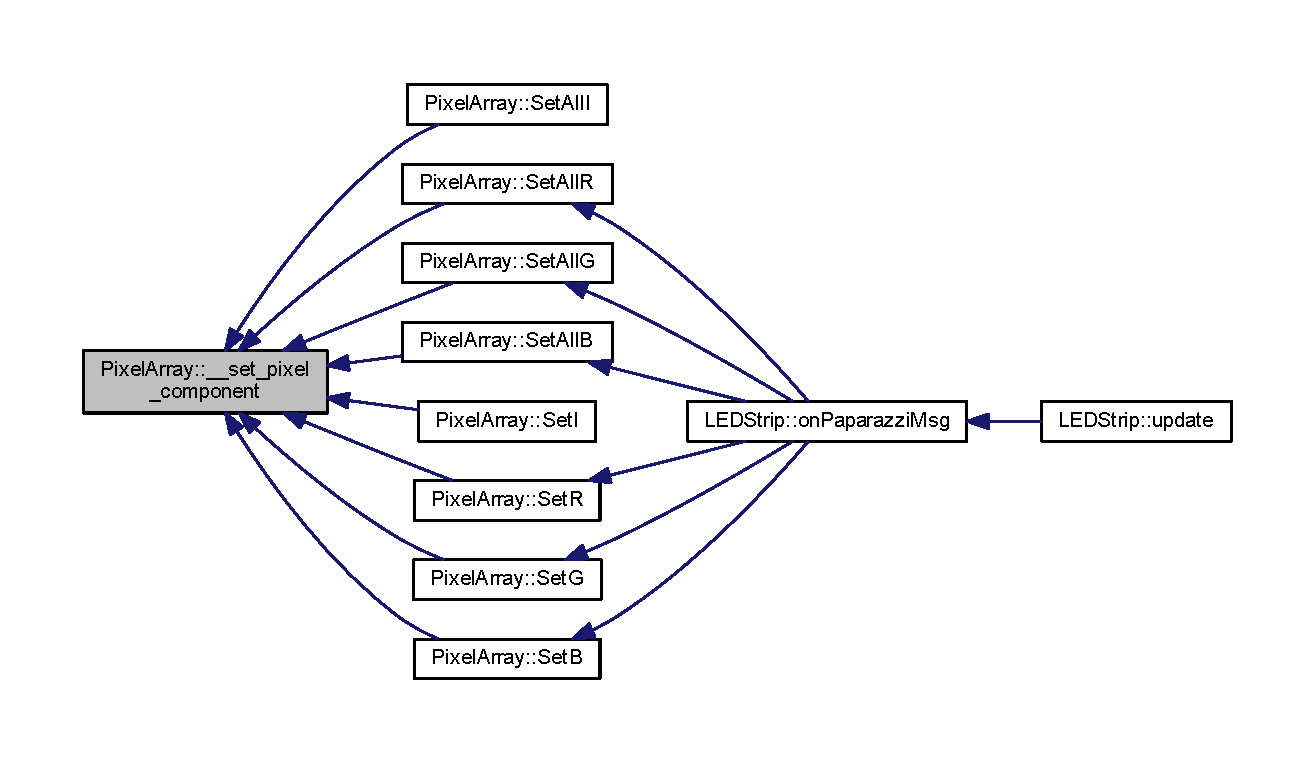
\includegraphics[width=350pt]{class_pixel_array_a42c6681bf771332826ecc9ad2a8cea02_icgraph}
\end{center}
\end{figure}
\mbox{\Hypertarget{class_pixel_array_a987f1dc053a5cf25d78d5cfe037088d3}\label{class_pixel_array_a987f1dc053a5cf25d78d5cfe037088d3}} 
\index{Pixel\+Array@{Pixel\+Array}!get\+Buf@{get\+Buf}}
\index{get\+Buf@{get\+Buf}!Pixel\+Array@{Pixel\+Array}}
\subsubsection{\texorpdfstring{get\+Buf()}{getBuf()}}
{\footnotesize\ttfamily int $\ast$ Pixel\+Array\+::get\+Buf (\begin{DoxyParamCaption}{ }\end{DoxyParamCaption})}



Definition at line 117 of file Pixel\+Array.\+cpp.


\begin{DoxyCode}
118 \{
119     \textcolor{keywordflow}{return} (\hyperlink{class_pixel_array_ab0109a336e69a9942b2723e43ee715d7}{pbuf});
120 \}
\end{DoxyCode}
Here is the caller graph for this function\+:\nopagebreak
\begin{figure}[H]
\begin{center}
\leavevmode
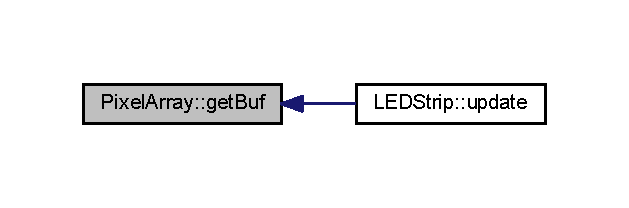
\includegraphics[width=302pt]{class_pixel_array_a987f1dc053a5cf25d78d5cfe037088d3_icgraph}
\end{center}
\end{figure}
\mbox{\Hypertarget{class_pixel_array_afcfe32b74beeced27f928f42131d77c1}\label{class_pixel_array_afcfe32b74beeced27f928f42131d77c1}} 
\index{Pixel\+Array@{Pixel\+Array}!Set@{Set}}
\index{Set@{Set}!Pixel\+Array@{Pixel\+Array}}
\subsubsection{\texorpdfstring{Set()}{Set()}}
{\footnotesize\ttfamily void Pixel\+Array\+::\+Set (\begin{DoxyParamCaption}\item[{int}]{i,  }\item[{unsigned int}]{value }\end{DoxyParamCaption})}



Definition at line 78 of file Pixel\+Array.\+cpp.


\begin{DoxyCode}
79 \{
80     \textcolor{keywordflow}{if} ((i >= 0) && (i < \hyperlink{class_pixel_array_aca29e70f9b643bff3733ab2e694439a1}{pbufsize})) \{
81         \hyperlink{class_pixel_array_a4b1a6582bc3bab1f67aebd1f97a5595d}{\_\_set\_pixel}(i,value);
82     \}
83 \}
\end{DoxyCode}
Here is the call graph for this function\+:\nopagebreak
\begin{figure}[H]
\begin{center}
\leavevmode
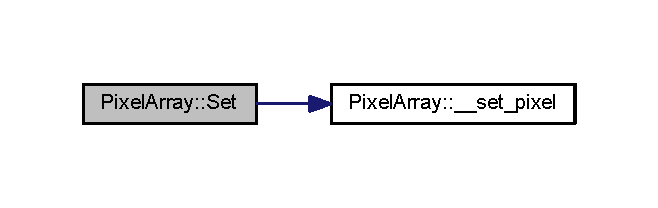
\includegraphics[width=316pt]{class_pixel_array_afcfe32b74beeced27f928f42131d77c1_cgraph}
\end{center}
\end{figure}
Here is the caller graph for this function\+:\nopagebreak
\begin{figure}[H]
\begin{center}
\leavevmode
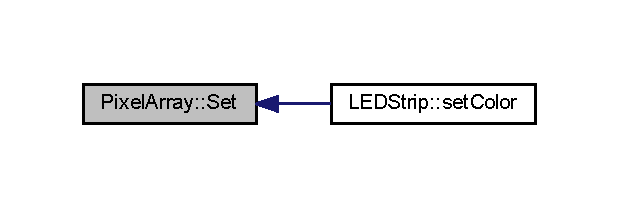
\includegraphics[width=297pt]{class_pixel_array_afcfe32b74beeced27f928f42131d77c1_icgraph}
\end{center}
\end{figure}
\mbox{\Hypertarget{class_pixel_array_a5f560dcef3d1582614858969b20da89d}\label{class_pixel_array_a5f560dcef3d1582614858969b20da89d}} 
\index{Pixel\+Array@{Pixel\+Array}!Set\+All@{Set\+All}}
\index{Set\+All@{Set\+All}!Pixel\+Array@{Pixel\+Array}}
\subsubsection{\texorpdfstring{Set\+All()}{SetAll()}}
{\footnotesize\ttfamily void Pixel\+Array\+::\+Set\+All (\begin{DoxyParamCaption}\item[{unsigned int}]{value }\end{DoxyParamCaption})}



Definition at line 25 of file Pixel\+Array.\+cpp.


\begin{DoxyCode}
26 \{
27     \textcolor{comment}{// for each pixel}
28     \textcolor{keywordflow}{for} (\textcolor{keywordtype}{int} i=0 ; i < \hyperlink{class_pixel_array_aca29e70f9b643bff3733ab2e694439a1}{pbufsize}; i++) \{
29         \hyperlink{class_pixel_array_a4b1a6582bc3bab1f67aebd1f97a5595d}{\_\_set\_pixel}(i,value);
30     \}
31 \}
\end{DoxyCode}
Here is the call graph for this function\+:\nopagebreak
\begin{figure}[H]
\begin{center}
\leavevmode
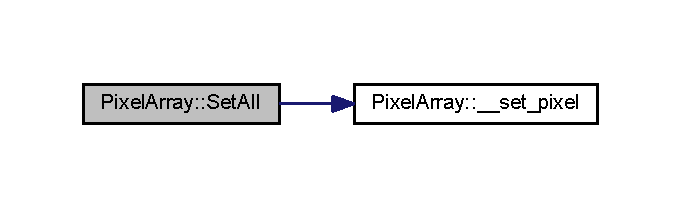
\includegraphics[width=327pt]{class_pixel_array_a5f560dcef3d1582614858969b20da89d_cgraph}
\end{center}
\end{figure}
Here is the caller graph for this function\+:\nopagebreak
\begin{figure}[H]
\begin{center}
\leavevmode
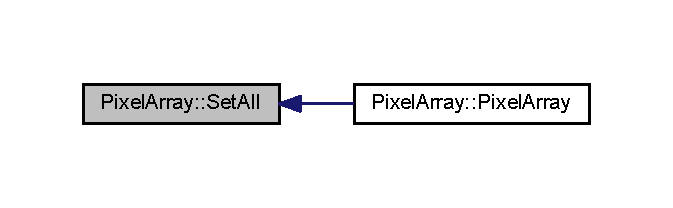
\includegraphics[width=323pt]{class_pixel_array_a5f560dcef3d1582614858969b20da89d_icgraph}
\end{center}
\end{figure}
\mbox{\Hypertarget{class_pixel_array_a3b17271fdc21503236ca6ca8e37d501b}\label{class_pixel_array_a3b17271fdc21503236ca6ca8e37d501b}} 
\index{Pixel\+Array@{Pixel\+Array}!Set\+AllB@{Set\+AllB}}
\index{Set\+AllB@{Set\+AllB}!Pixel\+Array@{Pixel\+Array}}
\subsubsection{\texorpdfstring{Set\+All\+B()}{SetAllB()}}
{\footnotesize\ttfamily void Pixel\+Array\+::\+Set\+AllB (\begin{DoxyParamCaption}\item[{unsigned char}]{value }\end{DoxyParamCaption})}



Definition at line 69 of file Pixel\+Array.\+cpp.


\begin{DoxyCode}
70 \{
71     \textcolor{comment}{// for each pixel}
72     \textcolor{keywordflow}{for} (\textcolor{keywordtype}{int} i=0 ; i < \hyperlink{class_pixel_array_aca29e70f9b643bff3733ab2e694439a1}{pbufsize}; i++) \{
73         \hyperlink{class_pixel_array_a42c6681bf771332826ecc9ad2a8cea02}{\_\_set\_pixel\_component}(i,0,value);
74     \}
75 \}
\end{DoxyCode}
Here is the call graph for this function\+:\nopagebreak
\begin{figure}[H]
\begin{center}
\leavevmode
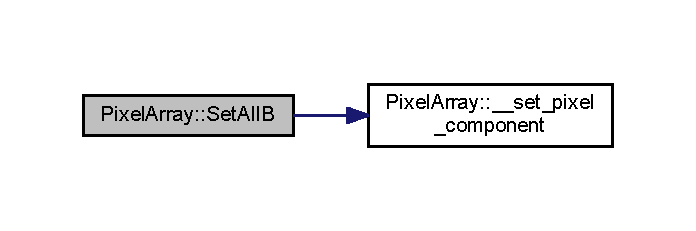
\includegraphics[width=334pt]{class_pixel_array_a3b17271fdc21503236ca6ca8e37d501b_cgraph}
\end{center}
\end{figure}
Here is the caller graph for this function\+:\nopagebreak
\begin{figure}[H]
\begin{center}
\leavevmode
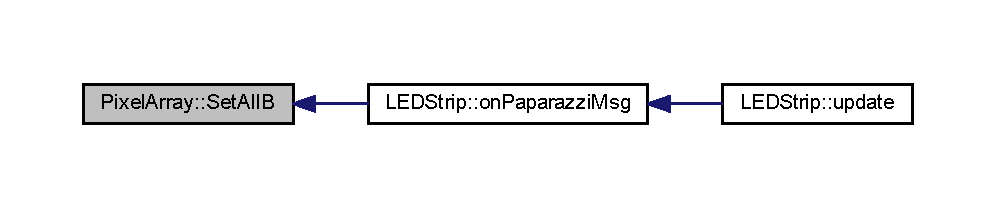
\includegraphics[width=350pt]{class_pixel_array_a3b17271fdc21503236ca6ca8e37d501b_icgraph}
\end{center}
\end{figure}
\mbox{\Hypertarget{class_pixel_array_a88f25ee1b266e2dc0ef7ae90ff4bd12d}\label{class_pixel_array_a88f25ee1b266e2dc0ef7ae90ff4bd12d}} 
\index{Pixel\+Array@{Pixel\+Array}!Set\+AllG@{Set\+AllG}}
\index{Set\+AllG@{Set\+AllG}!Pixel\+Array@{Pixel\+Array}}
\subsubsection{\texorpdfstring{Set\+All\+G()}{SetAllG()}}
{\footnotesize\ttfamily void Pixel\+Array\+::\+Set\+AllG (\begin{DoxyParamCaption}\item[{unsigned char}]{value }\end{DoxyParamCaption})}



Definition at line 57 of file Pixel\+Array.\+cpp.


\begin{DoxyCode}
58 \{
59     \textcolor{comment}{// for each pixel}
60     \textcolor{keywordflow}{for} (\textcolor{keywordtype}{int} i=0 ; i < \hyperlink{class_pixel_array_aca29e70f9b643bff3733ab2e694439a1}{pbufsize}; i++) \{
61         \hyperlink{class_pixel_array_a42c6681bf771332826ecc9ad2a8cea02}{\_\_set\_pixel\_component}(i,1,value);
62     \}
63 \}
\end{DoxyCode}
Here is the call graph for this function\+:\nopagebreak
\begin{figure}[H]
\begin{center}
\leavevmode
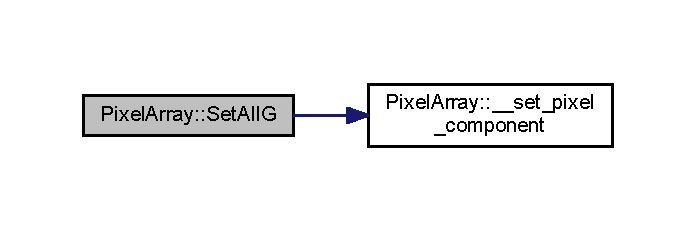
\includegraphics[width=334pt]{class_pixel_array_a88f25ee1b266e2dc0ef7ae90ff4bd12d_cgraph}
\end{center}
\end{figure}
Here is the caller graph for this function\+:\nopagebreak
\begin{figure}[H]
\begin{center}
\leavevmode
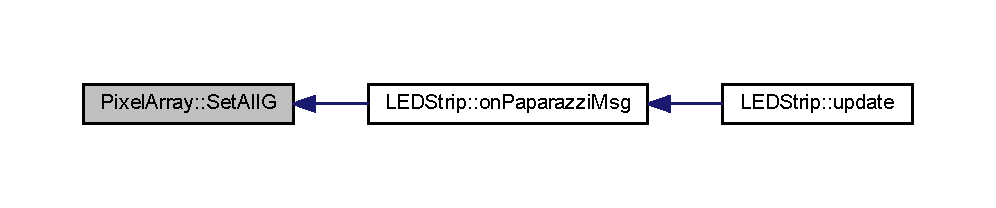
\includegraphics[width=350pt]{class_pixel_array_a88f25ee1b266e2dc0ef7ae90ff4bd12d_icgraph}
\end{center}
\end{figure}
\mbox{\Hypertarget{class_pixel_array_a9433e281c3cc0e4f8bbf23e127d8ad2c}\label{class_pixel_array_a9433e281c3cc0e4f8bbf23e127d8ad2c}} 
\index{Pixel\+Array@{Pixel\+Array}!Set\+AllI@{Set\+AllI}}
\index{Set\+AllI@{Set\+AllI}!Pixel\+Array@{Pixel\+Array}}
\subsubsection{\texorpdfstring{Set\+All\+I()}{SetAllI()}}
{\footnotesize\ttfamily void Pixel\+Array\+::\+Set\+AllI (\begin{DoxyParamCaption}\item[{unsigned char}]{value }\end{DoxyParamCaption})}



Definition at line 34 of file Pixel\+Array.\+cpp.


\begin{DoxyCode}
35 \{
36     \textcolor{comment}{// for each pixel}
37     \textcolor{keywordflow}{for} (\textcolor{keywordtype}{int} i=0 ; i < \hyperlink{class_pixel_array_aca29e70f9b643bff3733ab2e694439a1}{pbufsize}; i++) \{
38         \hyperlink{class_pixel_array_a42c6681bf771332826ecc9ad2a8cea02}{\_\_set\_pixel\_component}(i,3,value);
39     \}
40 \}
\end{DoxyCode}
Here is the call graph for this function\+:\nopagebreak
\begin{figure}[H]
\begin{center}
\leavevmode
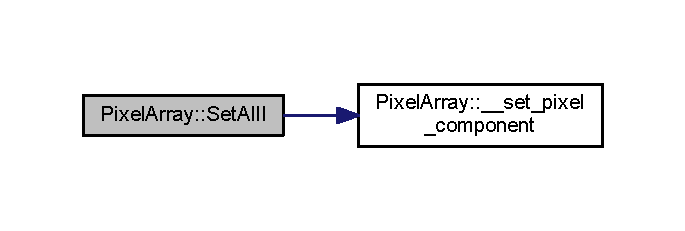
\includegraphics[width=329pt]{class_pixel_array_a9433e281c3cc0e4f8bbf23e127d8ad2c_cgraph}
\end{center}
\end{figure}
\mbox{\Hypertarget{class_pixel_array_a9ddfdd1a01a9877e4bfcf5a462412fd2}\label{class_pixel_array_a9ddfdd1a01a9877e4bfcf5a462412fd2}} 
\index{Pixel\+Array@{Pixel\+Array}!Set\+AllR@{Set\+AllR}}
\index{Set\+AllR@{Set\+AllR}!Pixel\+Array@{Pixel\+Array}}
\subsubsection{\texorpdfstring{Set\+All\+R()}{SetAllR()}}
{\footnotesize\ttfamily void Pixel\+Array\+::\+Set\+AllR (\begin{DoxyParamCaption}\item[{unsigned char}]{value }\end{DoxyParamCaption})}



Definition at line 46 of file Pixel\+Array.\+cpp.


\begin{DoxyCode}
47 \{
48     \textcolor{comment}{// for each pixel}
49     \textcolor{keywordflow}{for} (\textcolor{keywordtype}{int} i=0 ; i < \hyperlink{class_pixel_array_aca29e70f9b643bff3733ab2e694439a1}{pbufsize}; i++) \{
50         \hyperlink{class_pixel_array_a42c6681bf771332826ecc9ad2a8cea02}{\_\_set\_pixel\_component}(i,2,value);
51     \}
52 \}
\end{DoxyCode}
Here is the call graph for this function\+:\nopagebreak
\begin{figure}[H]
\begin{center}
\leavevmode
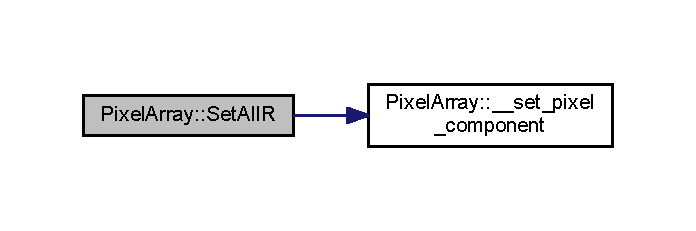
\includegraphics[width=334pt]{class_pixel_array_a9ddfdd1a01a9877e4bfcf5a462412fd2_cgraph}
\end{center}
\end{figure}
Here is the caller graph for this function\+:\nopagebreak
\begin{figure}[H]
\begin{center}
\leavevmode
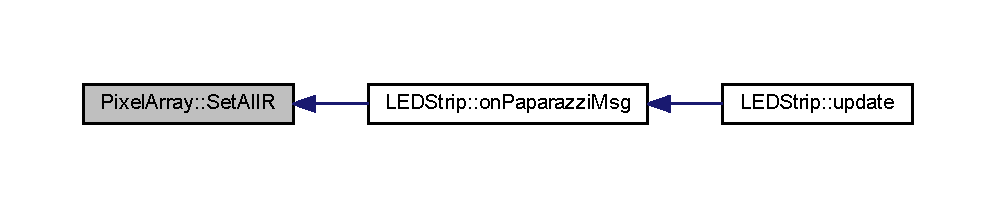
\includegraphics[width=350pt]{class_pixel_array_a9ddfdd1a01a9877e4bfcf5a462412fd2_icgraph}
\end{center}
\end{figure}
\mbox{\Hypertarget{class_pixel_array_a560a654c59614fd5a6c17adb10083a78}\label{class_pixel_array_a560a654c59614fd5a6c17adb10083a78}} 
\index{Pixel\+Array@{Pixel\+Array}!SetB@{SetB}}
\index{SetB@{SetB}!Pixel\+Array@{Pixel\+Array}}
\subsubsection{\texorpdfstring{Set\+B()}{SetB()}}
{\footnotesize\ttfamily void Pixel\+Array\+::\+SetB (\begin{DoxyParamCaption}\item[{int}]{i,  }\item[{unsigned char}]{value }\end{DoxyParamCaption})}



Definition at line 109 of file Pixel\+Array.\+cpp.


\begin{DoxyCode}
110 \{
111     \textcolor{keywordflow}{if} ((i >= 0) && (i < \hyperlink{class_pixel_array_aca29e70f9b643bff3733ab2e694439a1}{pbufsize})) \{
112         \hyperlink{class_pixel_array_a42c6681bf771332826ecc9ad2a8cea02}{\_\_set\_pixel\_component}(i,0,value);
113     \}
114 \}
\end{DoxyCode}
Here is the call graph for this function\+:\nopagebreak
\begin{figure}[H]
\begin{center}
\leavevmode
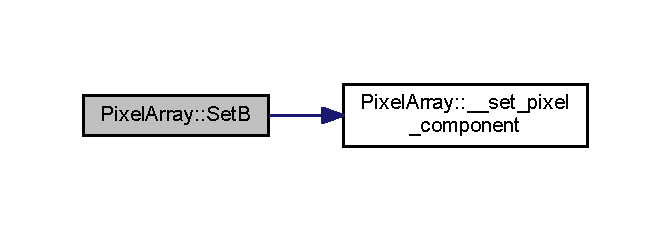
\includegraphics[width=322pt]{class_pixel_array_a560a654c59614fd5a6c17adb10083a78_cgraph}
\end{center}
\end{figure}
Here is the caller graph for this function\+:\nopagebreak
\begin{figure}[H]
\begin{center}
\leavevmode
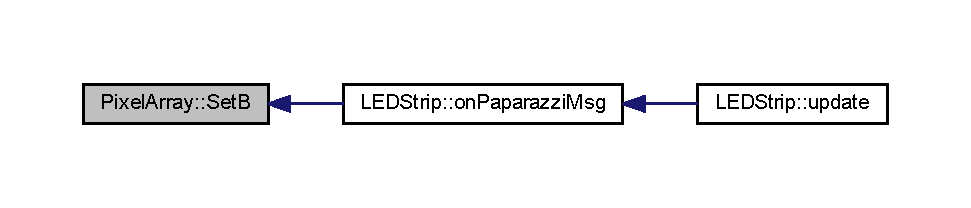
\includegraphics[width=350pt]{class_pixel_array_a560a654c59614fd5a6c17adb10083a78_icgraph}
\end{center}
\end{figure}
\mbox{\Hypertarget{class_pixel_array_a60ea8084ec95df0d51f46c9b0ff308d5}\label{class_pixel_array_a60ea8084ec95df0d51f46c9b0ff308d5}} 
\index{Pixel\+Array@{Pixel\+Array}!SetG@{SetG}}
\index{SetG@{SetG}!Pixel\+Array@{Pixel\+Array}}
\subsubsection{\texorpdfstring{Set\+G()}{SetG()}}
{\footnotesize\ttfamily void Pixel\+Array\+::\+SetG (\begin{DoxyParamCaption}\item[{int}]{i,  }\item[{unsigned char}]{value }\end{DoxyParamCaption})}



Definition at line 102 of file Pixel\+Array.\+cpp.


\begin{DoxyCode}
103 \{
104     \textcolor{keywordflow}{if} ((i >= 0) && (i < \hyperlink{class_pixel_array_aca29e70f9b643bff3733ab2e694439a1}{pbufsize})) \{
105         \hyperlink{class_pixel_array_a42c6681bf771332826ecc9ad2a8cea02}{\_\_set\_pixel\_component}(i,1,value);
106     \}
107 \}
\end{DoxyCode}
Here is the call graph for this function\+:\nopagebreak
\begin{figure}[H]
\begin{center}
\leavevmode
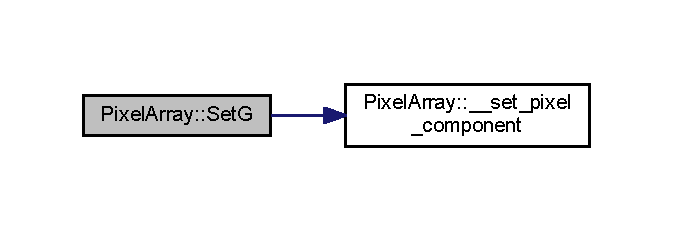
\includegraphics[width=323pt]{class_pixel_array_a60ea8084ec95df0d51f46c9b0ff308d5_cgraph}
\end{center}
\end{figure}
Here is the caller graph for this function\+:\nopagebreak
\begin{figure}[H]
\begin{center}
\leavevmode
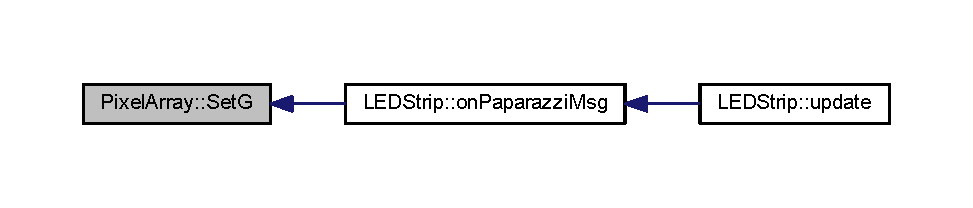
\includegraphics[width=350pt]{class_pixel_array_a60ea8084ec95df0d51f46c9b0ff308d5_icgraph}
\end{center}
\end{figure}
\mbox{\Hypertarget{class_pixel_array_afbfac74c674f63d793d85141d3a3b046}\label{class_pixel_array_afbfac74c674f63d793d85141d3a3b046}} 
\index{Pixel\+Array@{Pixel\+Array}!SetI@{SetI}}
\index{SetI@{SetI}!Pixel\+Array@{Pixel\+Array}}
\subsubsection{\texorpdfstring{Set\+I()}{SetI()}}
{\footnotesize\ttfamily void Pixel\+Array\+::\+SetI (\begin{DoxyParamCaption}\item[{int}]{i,  }\item[{unsigned char}]{value }\end{DoxyParamCaption})}



Definition at line 87 of file Pixel\+Array.\+cpp.


\begin{DoxyCode}
88 \{
89     \textcolor{keywordflow}{if} ((i >= 0) && (i < \hyperlink{class_pixel_array_aca29e70f9b643bff3733ab2e694439a1}{pbufsize})) \{
90         \hyperlink{class_pixel_array_a42c6681bf771332826ecc9ad2a8cea02}{\_\_set\_pixel\_component}(i,3,value);
91     \}
92 \}
\end{DoxyCode}
Here is the call graph for this function\+:\nopagebreak
\begin{figure}[H]
\begin{center}
\leavevmode
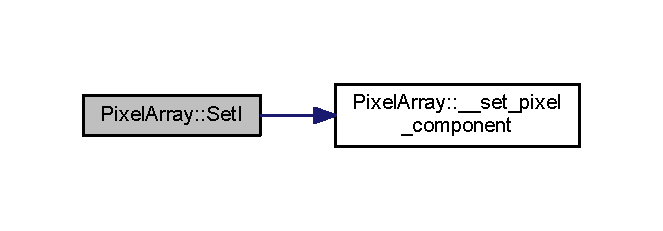
\includegraphics[width=318pt]{class_pixel_array_afbfac74c674f63d793d85141d3a3b046_cgraph}
\end{center}
\end{figure}
\mbox{\Hypertarget{class_pixel_array_abd4253e7c76f3775f31e09dfe318e3a5}\label{class_pixel_array_abd4253e7c76f3775f31e09dfe318e3a5}} 
\index{Pixel\+Array@{Pixel\+Array}!SetR@{SetR}}
\index{SetR@{SetR}!Pixel\+Array@{Pixel\+Array}}
\subsubsection{\texorpdfstring{Set\+R()}{SetR()}}
{\footnotesize\ttfamily void Pixel\+Array\+::\+SetR (\begin{DoxyParamCaption}\item[{int}]{i,  }\item[{unsigned char}]{value }\end{DoxyParamCaption})}



Definition at line 95 of file Pixel\+Array.\+cpp.


\begin{DoxyCode}
96 \{
97     \textcolor{keywordflow}{if} ((i >= 0) && (i < \hyperlink{class_pixel_array_aca29e70f9b643bff3733ab2e694439a1}{pbufsize})) \{
98         \hyperlink{class_pixel_array_a42c6681bf771332826ecc9ad2a8cea02}{\_\_set\_pixel\_component}(i,2,value);
99     \}
100 \}
\end{DoxyCode}
Here is the call graph for this function\+:\nopagebreak
\begin{figure}[H]
\begin{center}
\leavevmode
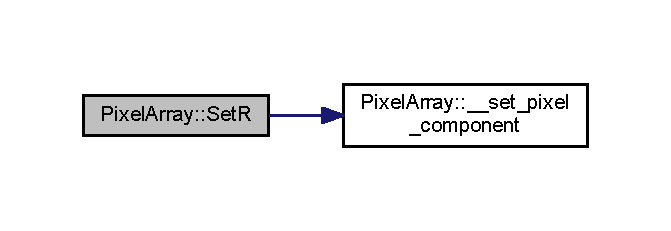
\includegraphics[width=322pt]{class_pixel_array_abd4253e7c76f3775f31e09dfe318e3a5_cgraph}
\end{center}
\end{figure}
Here is the caller graph for this function\+:\nopagebreak
\begin{figure}[H]
\begin{center}
\leavevmode
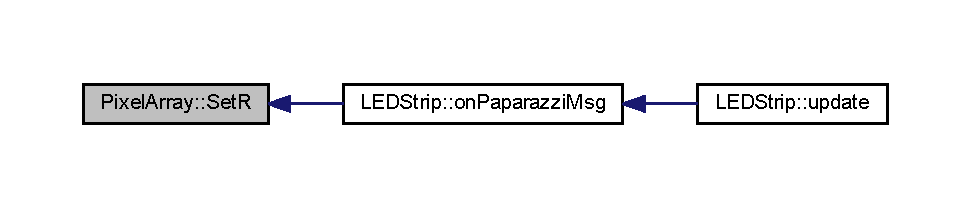
\includegraphics[width=350pt]{class_pixel_array_abd4253e7c76f3775f31e09dfe318e3a5_icgraph}
\end{center}
\end{figure}


\subsection{Member Data Documentation}
\mbox{\Hypertarget{class_pixel_array_ab0109a336e69a9942b2723e43ee715d7}\label{class_pixel_array_ab0109a336e69a9942b2723e43ee715d7}} 
\index{Pixel\+Array@{Pixel\+Array}!pbuf@{pbuf}}
\index{pbuf@{pbuf}!Pixel\+Array@{Pixel\+Array}}
\subsubsection{\texorpdfstring{pbuf}{pbuf}}
{\footnotesize\ttfamily int$\ast$ Pixel\+Array\+::pbuf\hspace{0.3cm}{\ttfamily [private]}}



Definition at line 41 of file Pixel\+Array.\+h.

\mbox{\Hypertarget{class_pixel_array_aca29e70f9b643bff3733ab2e694439a1}\label{class_pixel_array_aca29e70f9b643bff3733ab2e694439a1}} 
\index{Pixel\+Array@{Pixel\+Array}!pbufsize@{pbufsize}}
\index{pbufsize@{pbufsize}!Pixel\+Array@{Pixel\+Array}}
\subsubsection{\texorpdfstring{pbufsize}{pbufsize}}
{\footnotesize\ttfamily int Pixel\+Array\+::pbufsize\hspace{0.3cm}{\ttfamily [private]}}



Definition at line 42 of file Pixel\+Array.\+h.



The documentation for this class was generated from the following files\+:\begin{DoxyCompactItemize}
\item 
\hyperlink{_pixel_array_8h}{Pixel\+Array.\+h}\item 
\hyperlink{_pixel_array_8cpp}{Pixel\+Array.\+cpp}\end{DoxyCompactItemize}

\hypertarget{class_simple_l_e_d}{}\section{Simple\+L\+ED Class Reference}
\label{class_simple_l_e_d}\index{Simple\+L\+ED@{Simple\+L\+ED}}


{\ttfamily \#include $<$Simple\+L\+E\+D.\+h$>$}



Inheritance diagram for Simple\+L\+ED\+:\nopagebreak
\begin{figure}[H]
\begin{center}
\leavevmode
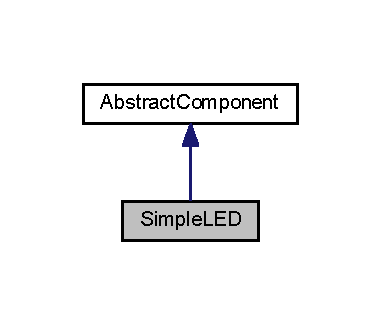
\includegraphics[width=183pt]{class_simple_l_e_d__inherit__graph}
\end{center}
\end{figure}


Collaboration diagram for Simple\+L\+ED\+:\nopagebreak
\begin{figure}[H]
\begin{center}
\leavevmode
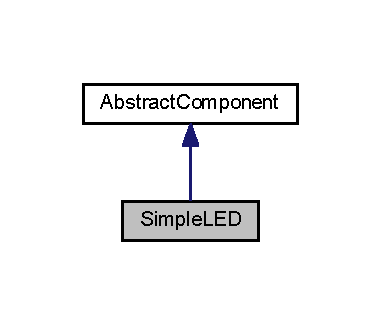
\includegraphics[width=183pt]{class_simple_l_e_d__coll__graph}
\end{center}
\end{figure}
\subsection*{Public Member Functions}
\begin{DoxyCompactItemize}
\item 
\hyperlink{class_simple_l_e_d_afec6f532dbc735f2fd95a2d080e7398d}{Simple\+L\+ED} (Pin\+Name out\+Pin)
\begin{DoxyCompactList}\small\item\em Simple blinking L\+ED. \end{DoxyCompactList}\item 
\hyperlink{class_simple_l_e_d_a035610e281499c6a1160b2ae6b2797f0}{Simple\+L\+ED} (Pin\+Name out\+Pin, int init\+Value)
\begin{DoxyCompactList}\small\item\em Simple blinking L\+ED. \end{DoxyCompactList}\item 
virtual void \hyperlink{class_simple_l_e_d_a1642dc4aca42ad46e5663a39cdda005f}{update} ()
\item 
void \hyperlink{class_abstract_component_a58a59a9ea6c3b4c86fb3bf98ff1eaaef}{set\+Priority} (int p)
\begin{DoxyCompactList}\small\item\em Set priority to the component, used for updating order. \end{DoxyCompactList}\item 
int \hyperlink{class_abstract_component_ac0b440d1d642ff1292ec3c544d75a8f1}{get\+Priority} ()
\item 
bool \hyperlink{class_abstract_component_a0c2e458144111c5f599c66f168516abc}{operator$<$} (const \hyperlink{class_abstract_component}{Abstract\+Component} \&another) const
\begin{DoxyCompactList}\small\item\em Overloaded comparison operator \textquotesingle{}$<$\textquotesingle{}. \end{DoxyCompactList}\end{DoxyCompactItemize}
\subsection*{Protected Attributes}
\begin{DoxyCompactItemize}
\item 
int \hyperlink{class_abstract_component_a9c9c548149681b1a1dd935e66ed5dd11}{id}
\item 
int \hyperlink{class_abstract_component_aff57dfa5f31be093a06b55560e33fb95}{priority} = 0
\end{DoxyCompactItemize}
\subsection*{Static Protected Attributes}
\begin{DoxyCompactItemize}
\item 
static int \hyperlink{class_abstract_component_a99ce3e5fe7d73dac569b874c15fcaf0d}{s\+\_\+id} = 0
\begin{DoxyCompactList}\small\item\em The id for each component will be created in a sequence order staring with 1. \end{DoxyCompactList}\end{DoxyCompactItemize}
\subsection*{Private Attributes}
\begin{DoxyCompactItemize}
\item 
Digital\+Out \hyperlink{class_simple_l_e_d_ae16514a63d8a19ab12e9adb19bba086d}{led}
\end{DoxyCompactItemize}


\subsection{Detailed Description}


Definition at line 5 of file Simple\+L\+E\+D.\+h.



\subsection{Constructor \& Destructor Documentation}
\mbox{\Hypertarget{class_simple_l_e_d_afec6f532dbc735f2fd95a2d080e7398d}\label{class_simple_l_e_d_afec6f532dbc735f2fd95a2d080e7398d}} 
\index{Simple\+L\+ED@{Simple\+L\+ED}!Simple\+L\+ED@{Simple\+L\+ED}}
\index{Simple\+L\+ED@{Simple\+L\+ED}!Simple\+L\+ED@{Simple\+L\+ED}}
\subsubsection{\texorpdfstring{Simple\+L\+E\+D()}{SimpleLED()}\hspace{0.1cm}{\footnotesize\ttfamily [1/2]}}
{\footnotesize\ttfamily Simple\+L\+E\+D\+::\+Simple\+L\+ED (\begin{DoxyParamCaption}\item[{Pin\+Name}]{out\+Pin }\end{DoxyParamCaption})}



Simple blinking L\+ED. 


\begin{DoxyParams}{Parameters}
{\em out\+Pin} & -\/ pin on board, where L\+ED is connected \\
\hline
\end{DoxyParams}


Definition at line 4 of file Simple\+L\+E\+D.\+cpp.


\begin{DoxyCode}
4                                   : \hyperlink{class_simple_l_e_d_ae16514a63d8a19ab12e9adb19bba086d}{led}(outPin) \{
5     \textcolor{keywordtype}{id} = ++\hyperlink{class_abstract_component_a99ce3e5fe7d73dac569b874c15fcaf0d}{s\_id};
6 \}
\end{DoxyCode}
\mbox{\Hypertarget{class_simple_l_e_d_a035610e281499c6a1160b2ae6b2797f0}\label{class_simple_l_e_d_a035610e281499c6a1160b2ae6b2797f0}} 
\index{Simple\+L\+ED@{Simple\+L\+ED}!Simple\+L\+ED@{Simple\+L\+ED}}
\index{Simple\+L\+ED@{Simple\+L\+ED}!Simple\+L\+ED@{Simple\+L\+ED}}
\subsubsection{\texorpdfstring{Simple\+L\+E\+D()}{SimpleLED()}\hspace{0.1cm}{\footnotesize\ttfamily [2/2]}}
{\footnotesize\ttfamily Simple\+L\+E\+D\+::\+Simple\+L\+ED (\begin{DoxyParamCaption}\item[{Pin\+Name}]{out\+Pin,  }\item[{int}]{init\+Value }\end{DoxyParamCaption})}



Simple blinking L\+ED. 


\begin{DoxyParams}{Parameters}
{\em out\+Pin} & -\/ pin on board, where L\+ED is connected \\
\hline
{\em init\+Value} & -\/ init value of the L\+ED, either -\/1 or 1 \\
\hline
\end{DoxyParams}


Definition at line 8 of file Simple\+L\+E\+D.\+cpp.


\begin{DoxyCode}
8 : \hyperlink{class_simple_l_e_d_ae16514a63d8a19ab12e9adb19bba086d}{led}(outPin, initValue) \{\}
\end{DoxyCode}


\subsection{Member Function Documentation}
\mbox{\Hypertarget{class_abstract_component_ac0b440d1d642ff1292ec3c544d75a8f1}\label{class_abstract_component_ac0b440d1d642ff1292ec3c544d75a8f1}} 
\index{Simple\+L\+ED@{Simple\+L\+ED}!get\+Priority@{get\+Priority}}
\index{get\+Priority@{get\+Priority}!Simple\+L\+ED@{Simple\+L\+ED}}
\subsubsection{\texorpdfstring{get\+Priority()}{getPriority()}}
{\footnotesize\ttfamily int Abstract\+Component\+::get\+Priority (\begin{DoxyParamCaption}{ }\end{DoxyParamCaption})\hspace{0.3cm}{\ttfamily [inline]}, {\ttfamily [inherited]}}

\begin{DoxyReturn}{Returns}
priority of the component 
\end{DoxyReturn}


Definition at line 25 of file Abstract\+Component.\+h.


\begin{DoxyCode}
25                       \{
26         \textcolor{keywordflow}{return} \hyperlink{class_abstract_component_aff57dfa5f31be093a06b55560e33fb95}{priority};
27     \}
\end{DoxyCode}
Here is the call graph for this function\+:
\nopagebreak
\begin{figure}[H]
\begin{center}
\leavevmode
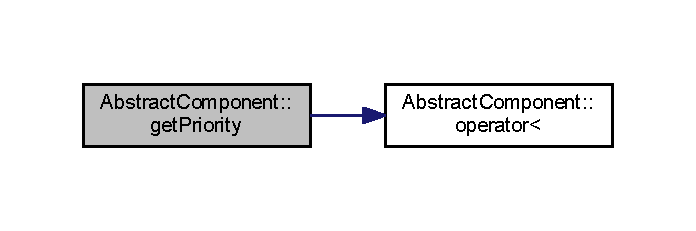
\includegraphics[width=334pt]{class_abstract_component_ac0b440d1d642ff1292ec3c544d75a8f1_cgraph}
\end{center}
\end{figure}
\mbox{\Hypertarget{class_abstract_component_a0c2e458144111c5f599c66f168516abc}\label{class_abstract_component_a0c2e458144111c5f599c66f168516abc}} 
\index{Simple\+L\+ED@{Simple\+L\+ED}!operator$<$@{operator$<$}}
\index{operator$<$@{operator$<$}!Simple\+L\+ED@{Simple\+L\+ED}}
\subsubsection{\texorpdfstring{operator$<$()}{operator<()}}
{\footnotesize\ttfamily bool Abstract\+Component\+::operator$<$ (\begin{DoxyParamCaption}\item[{const \hyperlink{class_abstract_component}{Abstract\+Component} \&}]{another }\end{DoxyParamCaption}) const\hspace{0.3cm}{\ttfamily [inherited]}}



Overloaded comparison operator \textquotesingle{}$<$\textquotesingle{}. 


\begin{DoxyParams}{Parameters}
{\em another} & component for comparison \\
\hline
\end{DoxyParams}
\begin{DoxyReturn}{Returns}
true if id is smaller then the id of another component 
\end{DoxyReturn}


Definition at line 8 of file Abstract\+Component.\+cpp.


\begin{DoxyCode}
8                                                                         \{
9     \textcolor{keywordflow}{return} \textcolor{keywordtype}{id} < another.\hyperlink{class_abstract_component_a9c9c548149681b1a1dd935e66ed5dd11}{id};
10 \}
\end{DoxyCode}
Here is the caller graph for this function\+:
\nopagebreak
\begin{figure}[H]
\begin{center}
\leavevmode
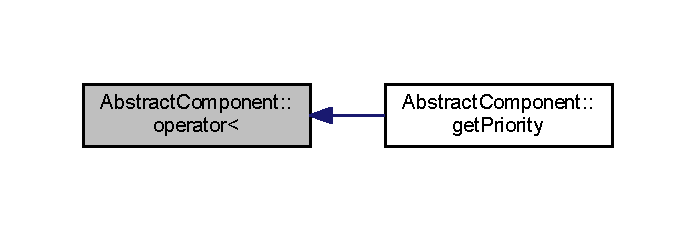
\includegraphics[width=334pt]{class_abstract_component_a0c2e458144111c5f599c66f168516abc_icgraph}
\end{center}
\end{figure}
\mbox{\Hypertarget{class_abstract_component_a58a59a9ea6c3b4c86fb3bf98ff1eaaef}\label{class_abstract_component_a58a59a9ea6c3b4c86fb3bf98ff1eaaef}} 
\index{Simple\+L\+ED@{Simple\+L\+ED}!set\+Priority@{set\+Priority}}
\index{set\+Priority@{set\+Priority}!Simple\+L\+ED@{Simple\+L\+ED}}
\subsubsection{\texorpdfstring{set\+Priority()}{setPriority()}}
{\footnotesize\ttfamily void Abstract\+Component\+::set\+Priority (\begin{DoxyParamCaption}\item[{int}]{p }\end{DoxyParamCaption})\hspace{0.3cm}{\ttfamily [inline]}, {\ttfamily [inherited]}}



Set priority to the component, used for updating order. 


\begin{DoxyParams}{Parameters}
{\em p} & priority \\
\hline
\end{DoxyParams}


Definition at line 18 of file Abstract\+Component.\+h.


\begin{DoxyCode}
18                             \{
19         \hyperlink{class_abstract_component_aff57dfa5f31be093a06b55560e33fb95}{priority} = p;
20     \}
\end{DoxyCode}
\mbox{\Hypertarget{class_simple_l_e_d_a1642dc4aca42ad46e5663a39cdda005f}\label{class_simple_l_e_d_a1642dc4aca42ad46e5663a39cdda005f}} 
\index{Simple\+L\+ED@{Simple\+L\+ED}!update@{update}}
\index{update@{update}!Simple\+L\+ED@{Simple\+L\+ED}}
\subsubsection{\texorpdfstring{update()}{update()}}
{\footnotesize\ttfamily void Simple\+L\+E\+D\+::update (\begin{DoxyParamCaption}{ }\end{DoxyParamCaption})\hspace{0.3cm}{\ttfamily [virtual]}}



Implements \hyperlink{class_abstract_component_af25a90b8ab213762221c3b358d9873f3}{Abstract\+Component}.



Definition at line 10 of file Simple\+L\+E\+D.\+cpp.


\begin{DoxyCode}
10                        \{
11     \hyperlink{class_simple_l_e_d_ae16514a63d8a19ab12e9adb19bba086d}{led} = !\hyperlink{class_simple_l_e_d_ae16514a63d8a19ab12e9adb19bba086d}{led};
12 \}
\end{DoxyCode}


\subsection{Member Data Documentation}
\mbox{\Hypertarget{class_abstract_component_a9c9c548149681b1a1dd935e66ed5dd11}\label{class_abstract_component_a9c9c548149681b1a1dd935e66ed5dd11}} 
\index{Simple\+L\+ED@{Simple\+L\+ED}!id@{id}}
\index{id@{id}!Simple\+L\+ED@{Simple\+L\+ED}}
\subsubsection{\texorpdfstring{id}{id}}
{\footnotesize\ttfamily int Abstract\+Component\+::id\hspace{0.3cm}{\ttfamily [protected]}, {\ttfamily [inherited]}}



Definition at line 39 of file Abstract\+Component.\+h.

\mbox{\Hypertarget{class_simple_l_e_d_ae16514a63d8a19ab12e9adb19bba086d}\label{class_simple_l_e_d_ae16514a63d8a19ab12e9adb19bba086d}} 
\index{Simple\+L\+ED@{Simple\+L\+ED}!led@{led}}
\index{led@{led}!Simple\+L\+ED@{Simple\+L\+ED}}
\subsubsection{\texorpdfstring{led}{led}}
{\footnotesize\ttfamily Digital\+Out Simple\+L\+E\+D\+::led\hspace{0.3cm}{\ttfamily [private]}}



Definition at line 25 of file Simple\+L\+E\+D.\+h.

\mbox{\Hypertarget{class_abstract_component_aff57dfa5f31be093a06b55560e33fb95}\label{class_abstract_component_aff57dfa5f31be093a06b55560e33fb95}} 
\index{Simple\+L\+ED@{Simple\+L\+ED}!priority@{priority}}
\index{priority@{priority}!Simple\+L\+ED@{Simple\+L\+ED}}
\subsubsection{\texorpdfstring{priority}{priority}}
{\footnotesize\ttfamily int Abstract\+Component\+::priority = 0\hspace{0.3cm}{\ttfamily [protected]}, {\ttfamily [inherited]}}



Definition at line 40 of file Abstract\+Component.\+h.

\mbox{\Hypertarget{class_abstract_component_a99ce3e5fe7d73dac569b874c15fcaf0d}\label{class_abstract_component_a99ce3e5fe7d73dac569b874c15fcaf0d}} 
\index{Simple\+L\+ED@{Simple\+L\+ED}!s\+\_\+id@{s\+\_\+id}}
\index{s\+\_\+id@{s\+\_\+id}!Simple\+L\+ED@{Simple\+L\+ED}}
\subsubsection{\texorpdfstring{s\+\_\+id}{s\_id}}
{\footnotesize\ttfamily int Abstract\+Component\+::s\+\_\+id = 0\hspace{0.3cm}{\ttfamily [static]}, {\ttfamily [protected]}, {\ttfamily [inherited]}}



The id for each component will be created in a sequence order staring with 1. 



Definition at line 38 of file Abstract\+Component.\+h.



The documentation for this class was generated from the following files\+:\begin{DoxyCompactItemize}
\item 
\hyperlink{_simple_l_e_d_8h}{Simple\+L\+E\+D.\+h}\item 
\hyperlink{_simple_l_e_d_8cpp}{Simple\+L\+E\+D.\+cpp}\end{DoxyCompactItemize}

\hypertarget{class_sonar}{}\section{Sonar Class Reference}
\label{class_sonar}\index{Sonar@{Sonar}}


{\ttfamily \#include $<$Sonar.\+h$>$}



Inheritance diagram for Sonar\+:\nopagebreak
\begin{figure}[H]
\begin{center}
\leavevmode
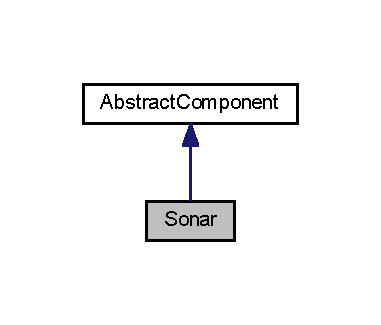
\includegraphics[width=183pt]{class_sonar__inherit__graph}
\end{center}
\end{figure}


Collaboration diagram for Sonar\+:\nopagebreak
\begin{figure}[H]
\begin{center}
\leavevmode
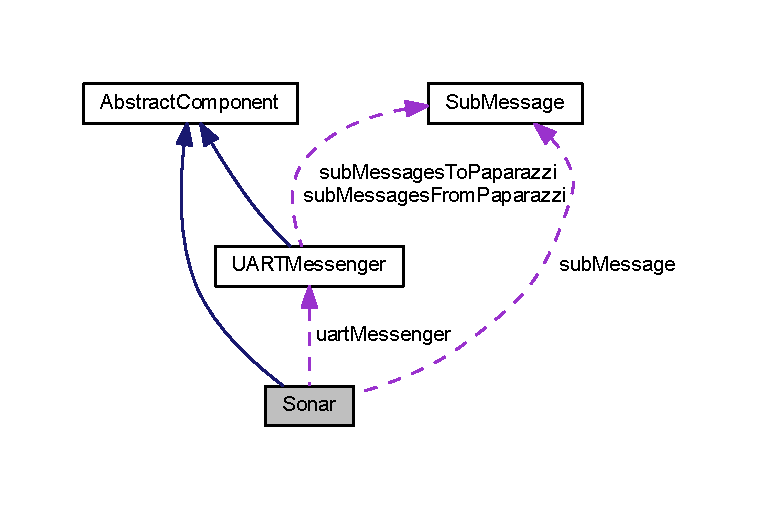
\includegraphics[width=350pt]{class_sonar__coll__graph}
\end{center}
\end{figure}
\subsection*{Public Member Functions}
\begin{DoxyCompactItemize}
\item 
\hyperlink{class_sonar_a8199e2b1d48626cc0404708063d7fe42}{Sonar} (\hyperlink{class_u_a_r_t_messenger}{U\+A\+R\+T\+Messenger} $\ast$const uart\+Msngr, uint8\+\_\+t addr, Event\+Queue $\ast$const \hyperlink{class_sonar_af0431d160853c8313eba0fd0e1ce8346}{queue})
\begin{DoxyCompactList}\small\item\em Constructor for \hyperlink{class_sonar}{Sonar}. \end{DoxyCompactList}\item 
virtual void \hyperlink{class_sonar_aaf10dd734528b86b4dea3ab35c4ee4f4}{update} ()
\begin{DoxyCompactList}\small\item\em Write value to i2c for the sonar. \end{DoxyCompactList}\item 
uint16\+\_\+t \hyperlink{class_sonar_a7a641bcfac1967fbc42eea2ab70886dc}{get\+Range} ()
\item 
void \hyperlink{class_abstract_component_a58a59a9ea6c3b4c86fb3bf98ff1eaaef}{set\+Priority} (int p)
\begin{DoxyCompactList}\small\item\em Set priority to the component, used for updating order. \end{DoxyCompactList}\item 
int \hyperlink{class_abstract_component_ac0b440d1d642ff1292ec3c544d75a8f1}{get\+Priority} ()
\item 
bool \hyperlink{class_abstract_component_a0c2e458144111c5f599c66f168516abc}{operator$<$} (const \hyperlink{class_abstract_component}{Abstract\+Component} \&another) const
\begin{DoxyCompactList}\small\item\em Overloaded comparison operator \textquotesingle{}$<$\textquotesingle{}. \end{DoxyCompactList}\end{DoxyCompactItemize}
\subsection*{Protected Attributes}
\begin{DoxyCompactItemize}
\item 
int \hyperlink{class_abstract_component_a9c9c548149681b1a1dd935e66ed5dd11}{id}
\item 
int \hyperlink{class_abstract_component_aff57dfa5f31be093a06b55560e33fb95}{priority} = 0
\end{DoxyCompactItemize}
\subsection*{Static Protected Attributes}
\begin{DoxyCompactItemize}
\item 
static int \hyperlink{class_abstract_component_a99ce3e5fe7d73dac569b874c15fcaf0d}{s\+\_\+id} = 0
\begin{DoxyCompactList}\small\item\em The id for each component will be created in a sequence order staring with 1. \end{DoxyCompactList}\end{DoxyCompactItemize}
\subsection*{Private Member Functions}
\begin{DoxyCompactItemize}
\item 
void \hyperlink{class_sonar_af7a8bb36d925d164b31ff271f9006dc7}{read} ()
\begin{DoxyCompactList}\small\item\em Read the range and then bit will be shifted towards left 8 bytes. \end{DoxyCompactList}\end{DoxyCompactItemize}
\subsection*{Private Attributes}
\begin{DoxyCompactItemize}
\item 
\hyperlink{class_u_a_r_t_messenger}{U\+A\+R\+T\+Messenger} $\ast$const \hyperlink{class_sonar_a63b5d2455e9278c9d3c6dded215789f6}{uart\+Messenger}
\item 
Event\+Queue $\ast$const \hyperlink{class_sonar_af0431d160853c8313eba0fd0e1ce8346}{queue}
\item 
\hyperlink{struct_sub_message}{Sub\+Message} \hyperlink{class_sonar_a08f09f7abe342846e6e97b8dd76d623b}{sub\+Message}
\item 
I2C \hyperlink{class_sonar_ae6be174d7fc69e27ae5d932b26a5a003}{i2c}
\item 
uint8\+\_\+t \hyperlink{class_sonar_aa42fef5da4ff8d80353143a74eff2ae2}{address}
\item 
char \hyperlink{class_sonar_a6a5dc5e466fc0c7a8cb2fc50af10db45}{config} \mbox{[}2\mbox{]}
\item 
uint16\+\_\+t \hyperlink{class_sonar_a6b0f78a9151925ca61fe54c852c195bd}{range}
\item 
Timeout \hyperlink{class_sonar_a4b3cc5317263c63dd58195f3c2c94da6}{timeout}
\end{DoxyCompactItemize}


\subsection{Detailed Description}


Definition at line 7 of file Sonar.\+h.



\subsection{Constructor \& Destructor Documentation}
\mbox{\Hypertarget{class_sonar_a8199e2b1d48626cc0404708063d7fe42}\label{class_sonar_a8199e2b1d48626cc0404708063d7fe42}} 
\index{Sonar@{Sonar}!Sonar@{Sonar}}
\index{Sonar@{Sonar}!Sonar@{Sonar}}
\subsubsection{\texorpdfstring{Sonar()}{Sonar()}}
{\footnotesize\ttfamily Sonar\+::\+Sonar (\begin{DoxyParamCaption}\item[{\hyperlink{class_u_a_r_t_messenger}{U\+A\+R\+T\+Messenger} $\ast$const}]{uart\+Msngr,  }\item[{uint8\+\_\+t}]{addr,  }\item[{Event\+Queue $\ast$const}]{queue }\end{DoxyParamCaption})}



Constructor for \hyperlink{class_sonar}{Sonar}. 


\begin{DoxyParams}{Parameters}
{\em uart\+Msngr} & Pointer to \hyperlink{class_u_a_r_t_messenger}{U\+A\+R\+T\+Messenger} object, that should be used for sending data to Paparazzi \\
\hline
{\em addr} & Address of the \hyperlink{class_sonar}{Sonar} \\
\hline
{\em queue} & mbed Event\+Queue \\
\hline
\end{DoxyParams}


Definition at line 9 of file Sonar.\+cpp.


\begin{DoxyCode}
9                                                                                   : 
      \hyperlink{class_sonar_a63b5d2455e9278c9d3c6dded215789f6}{uartMessenger}(uartMsngr), \hyperlink{class_sonar_af0431d160853c8313eba0fd0e1ce8346}{queue}(\hyperlink{class_sonar_af0431d160853c8313eba0fd0e1ce8346}{queue}), \hyperlink{class_sonar_ae6be174d7fc69e27ae5d932b26a5a003}{i2c}(I2C\_SDA, I2C\_SCL) \{
10     \textcolor{keywordtype}{id} = ++\hyperlink{class_abstract_component_a99ce3e5fe7d73dac569b874c15fcaf0d}{s\_id};
11     \hyperlink{class_sonar_ae6be174d7fc69e27ae5d932b26a5a003}{i2c}.frequency(50000);
12     \hyperlink{class_sonar_aa42fef5da4ff8d80353143a74eff2ae2}{address} = addr << 1;
13 \}
\end{DoxyCode}


\subsection{Member Function Documentation}
\mbox{\Hypertarget{class_abstract_component_ac0b440d1d642ff1292ec3c544d75a8f1}\label{class_abstract_component_ac0b440d1d642ff1292ec3c544d75a8f1}} 
\index{Sonar@{Sonar}!get\+Priority@{get\+Priority}}
\index{get\+Priority@{get\+Priority}!Sonar@{Sonar}}
\subsubsection{\texorpdfstring{get\+Priority()}{getPriority()}}
{\footnotesize\ttfamily int Abstract\+Component\+::get\+Priority (\begin{DoxyParamCaption}{ }\end{DoxyParamCaption})\hspace{0.3cm}{\ttfamily [inline]}, {\ttfamily [inherited]}}

\begin{DoxyReturn}{Returns}
priority of the component 
\end{DoxyReturn}


Definition at line 25 of file Abstract\+Component.\+h.


\begin{DoxyCode}
25                       \{
26         \textcolor{keywordflow}{return} \hyperlink{class_abstract_component_aff57dfa5f31be093a06b55560e33fb95}{priority};
27     \}
\end{DoxyCode}
Here is the call graph for this function\+:
\nopagebreak
\begin{figure}[H]
\begin{center}
\leavevmode
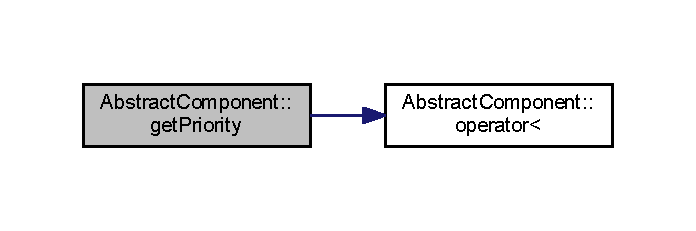
\includegraphics[width=334pt]{class_abstract_component_ac0b440d1d642ff1292ec3c544d75a8f1_cgraph}
\end{center}
\end{figure}
\mbox{\Hypertarget{class_sonar_a7a641bcfac1967fbc42eea2ab70886dc}\label{class_sonar_a7a641bcfac1967fbc42eea2ab70886dc}} 
\index{Sonar@{Sonar}!get\+Range@{get\+Range}}
\index{get\+Range@{get\+Range}!Sonar@{Sonar}}
\subsubsection{\texorpdfstring{get\+Range()}{getRange()}}
{\footnotesize\ttfamily uint16\+\_\+t Sonar\+::get\+Range (\begin{DoxyParamCaption}{ }\end{DoxyParamCaption})}

\begin{DoxyReturn}{Returns}
current range of this sensor 
\end{DoxyReturn}


Definition at line 52 of file Sonar.\+cpp.


\begin{DoxyCode}
52                          \{
53     \textcolor{keywordflow}{return} \hyperlink{class_sonar_a6b0f78a9151925ca61fe54c852c195bd}{range};
54 \}
\end{DoxyCode}
\mbox{\Hypertarget{class_abstract_component_a0c2e458144111c5f599c66f168516abc}\label{class_abstract_component_a0c2e458144111c5f599c66f168516abc}} 
\index{Sonar@{Sonar}!operator$<$@{operator$<$}}
\index{operator$<$@{operator$<$}!Sonar@{Sonar}}
\subsubsection{\texorpdfstring{operator$<$()}{operator<()}}
{\footnotesize\ttfamily bool Abstract\+Component\+::operator$<$ (\begin{DoxyParamCaption}\item[{const \hyperlink{class_abstract_component}{Abstract\+Component} \&}]{another }\end{DoxyParamCaption}) const\hspace{0.3cm}{\ttfamily [inherited]}}



Overloaded comparison operator \textquotesingle{}$<$\textquotesingle{}. 


\begin{DoxyParams}{Parameters}
{\em another} & component for comparison \\
\hline
\end{DoxyParams}
\begin{DoxyReturn}{Returns}
true if id is smaller then the id of another component 
\end{DoxyReturn}


Definition at line 8 of file Abstract\+Component.\+cpp.


\begin{DoxyCode}
8                                                                         \{
9     \textcolor{keywordflow}{return} \textcolor{keywordtype}{id} < another.\hyperlink{class_abstract_component_a9c9c548149681b1a1dd935e66ed5dd11}{id};
10 \}
\end{DoxyCode}
Here is the caller graph for this function\+:\nopagebreak
\begin{figure}[H]
\begin{center}
\leavevmode
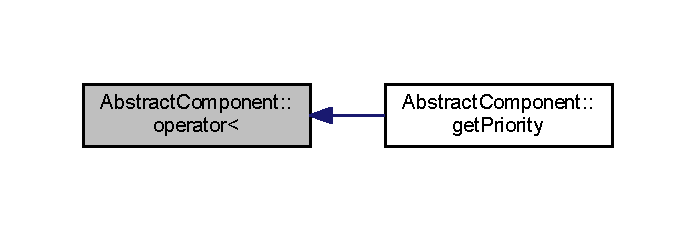
\includegraphics[width=334pt]{class_abstract_component_a0c2e458144111c5f599c66f168516abc_icgraph}
\end{center}
\end{figure}
\mbox{\Hypertarget{class_sonar_af7a8bb36d925d164b31ff271f9006dc7}\label{class_sonar_af7a8bb36d925d164b31ff271f9006dc7}} 
\index{Sonar@{Sonar}!read@{read}}
\index{read@{read}!Sonar@{Sonar}}
\subsubsection{\texorpdfstring{read()}{read()}}
{\footnotesize\ttfamily void Sonar\+::read (\begin{DoxyParamCaption}{ }\end{DoxyParamCaption})\hspace{0.3cm}{\ttfamily [private]}}



Read the range and then bit will be shifted towards left 8 bytes. 

Type of the sensor is S\+O\+N\+AR, id of the sensor, converting to data range to uint16\+\_\+t, length of the range. Appends the message to uart list. 

Definition at line 35 of file Sonar.\+cpp.


\begin{DoxyCode}
35                  \{
36     \hyperlink{class_sonar_ae6be174d7fc69e27ae5d932b26a5a003}{i2c}.lock();
37     \textcolor{keywordtype}{char} range\_read[2];
38     \textcolor{keywordtype}{int} a = \hyperlink{class_sonar_ae6be174d7fc69e27ae5d932b26a5a003}{i2c}.read(\hyperlink{class_sonar_aa42fef5da4ff8d80353143a74eff2ae2}{address} | 0x01, range\_read, 2); \textcolor{comment}{//read the two-byte range data}
39     \textcolor{keywordflow}{if} (a != 0)
40         \textcolor{keywordflow}{return}; \textcolor{comment}{// Reading failed}
41     \hyperlink{class_sonar_a6b0f78a9151925ca61fe54c852c195bd}{range} = ((range\_read[0] << 8) | range\_read[1]);
42     \hyperlink{class_sonar_ae6be174d7fc69e27ae5d932b26a5a003}{i2c}.unlock();
43 
44     \hyperlink{class_sonar_a08f09f7abe342846e6e97b8dd76d623b}{subMessage}.\hyperlink{struct_sub_message_a064f1d26d553da776dc749d37a18a499}{type} = \hyperlink{_sub_message_8h_a81f78fc173dedefe5a049c0aa3eed2c0a4cc68226cf454df7dd46f74f2a18d240}{SONAR};
45     \hyperlink{class_sonar_a08f09f7abe342846e6e97b8dd76d623b}{subMessage}.\hyperlink{struct_sub_message_af3acc450c0686d7a9d15ccd9d548cb6d}{id} = \hyperlink{class_abstract_component_a9c9c548149681b1a1dd935e66ed5dd11}{id};
46     \textcolor{keyword}{reinterpret\_cast<}uint16\_t *\textcolor{keyword}{>}(\hyperlink{class_sonar_a08f09f7abe342846e6e97b8dd76d623b}{subMessage}.\hyperlink{struct_sub_message_a7d923c5cdaa380c27d7c4cf60ea7c1be}{data})[0] = \hyperlink{class_sonar_a6b0f78a9151925ca61fe54c852c195bd}{range};
47     \hyperlink{class_sonar_a08f09f7abe342846e6e97b8dd76d623b}{subMessage}.\hyperlink{struct_sub_message_a276e06f5335ca7857c21ac8c0e51bd6d}{length} = \textcolor{keyword}{sizeof}(\hyperlink{class_sonar_a6b0f78a9151925ca61fe54c852c195bd}{range});
48 
49     \hyperlink{class_sonar_a63b5d2455e9278c9d3c6dded215789f6}{uartMessenger}->\hyperlink{class_u_a_r_t_messenger_ada0967869e320c236a211b405abf128a}{appendMessage}(\hyperlink{class_sonar_a08f09f7abe342846e6e97b8dd76d623b}{subMessage});
50 \}
\end{DoxyCode}
Here is the call graph for this function\+:\nopagebreak
\begin{figure}[H]
\begin{center}
\leavevmode
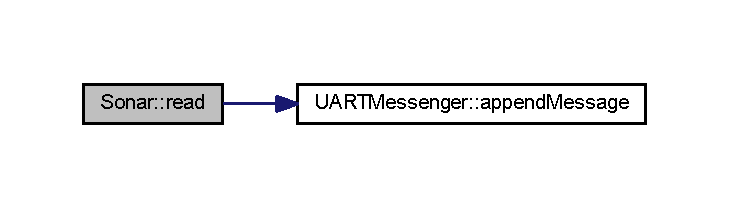
\includegraphics[width=350pt]{class_sonar_af7a8bb36d925d164b31ff271f9006dc7_cgraph}
\end{center}
\end{figure}
Here is the caller graph for this function\+:\nopagebreak
\begin{figure}[H]
\begin{center}
\leavevmode
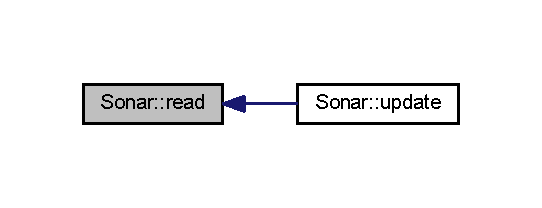
\includegraphics[width=260pt]{class_sonar_af7a8bb36d925d164b31ff271f9006dc7_icgraph}
\end{center}
\end{figure}
\mbox{\Hypertarget{class_abstract_component_a58a59a9ea6c3b4c86fb3bf98ff1eaaef}\label{class_abstract_component_a58a59a9ea6c3b4c86fb3bf98ff1eaaef}} 
\index{Sonar@{Sonar}!set\+Priority@{set\+Priority}}
\index{set\+Priority@{set\+Priority}!Sonar@{Sonar}}
\subsubsection{\texorpdfstring{set\+Priority()}{setPriority()}}
{\footnotesize\ttfamily void Abstract\+Component\+::set\+Priority (\begin{DoxyParamCaption}\item[{int}]{p }\end{DoxyParamCaption})\hspace{0.3cm}{\ttfamily [inline]}, {\ttfamily [inherited]}}



Set priority to the component, used for updating order. 


\begin{DoxyParams}{Parameters}
{\em p} & priority \\
\hline
\end{DoxyParams}


Definition at line 18 of file Abstract\+Component.\+h.


\begin{DoxyCode}
18                             \{
19         \hyperlink{class_abstract_component_aff57dfa5f31be093a06b55560e33fb95}{priority} = p;
20     \}
\end{DoxyCode}
\mbox{\Hypertarget{class_sonar_aaf10dd734528b86b4dea3ab35c4ee4f4}\label{class_sonar_aaf10dd734528b86b4dea3ab35c4ee4f4}} 
\index{Sonar@{Sonar}!update@{update}}
\index{update@{update}!Sonar@{Sonar}}
\subsubsection{\texorpdfstring{update()}{update()}}
{\footnotesize\ttfamily void Sonar\+::update (\begin{DoxyParamCaption}{ }\end{DoxyParamCaption})\hspace{0.3cm}{\ttfamily [virtual]}}



Write value to i2c for the sonar. 



Implements \hyperlink{class_abstract_component_af25a90b8ab213762221c3b358d9873f3}{Abstract\+Component}.



Definition at line 18 of file Sonar.\+cpp.


\begin{DoxyCode}
18                    \{
19     \hyperlink{class_sonar_ae6be174d7fc69e27ae5d932b26a5a003}{i2c}.lock();
20     \hyperlink{class_sonar_a6a5dc5e466fc0c7a8cb2fc50af10db45}{config}[0] = 0x51; \textcolor{comment}{//initializing the address as 81}
21     \textcolor{keywordtype}{int} a = \hyperlink{class_sonar_ae6be174d7fc69e27ae5d932b26a5a003}{i2c}.write(\hyperlink{class_sonar_aa42fef5da4ff8d80353143a74eff2ae2}{address} & ~1, \hyperlink{class_sonar_a6a5dc5e466fc0c7a8cb2fc50af10db45}{config}, 1);
22     \textcolor{keywordflow}{if} (a != 0)
23         \textcolor{keywordflow}{return}; \textcolor{comment}{// Writing failed}
24     \hyperlink{class_sonar_ae6be174d7fc69e27ae5d932b26a5a003}{i2c}.unlock();
25 
26     \textcolor{comment}{// move read function to the queue to be called after 80 ms}
27     \hyperlink{class_sonar_af0431d160853c8313eba0fd0e1ce8346}{queue}->call\_in(80, callback(\textcolor{keyword}{this}, &\hyperlink{class_sonar_af7a8bb36d925d164b31ff271f9006dc7}{Sonar::read}));
28 \}
\end{DoxyCode}
Here is the call graph for this function\+:\nopagebreak
\begin{figure}[H]
\begin{center}
\leavevmode
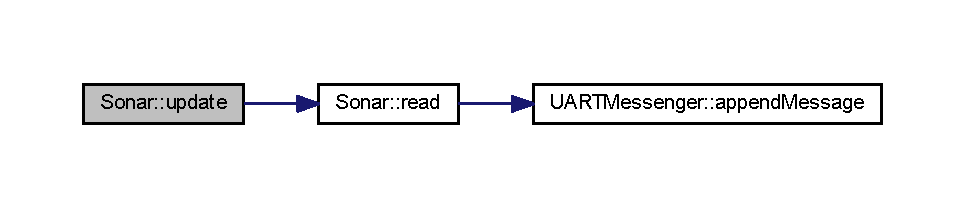
\includegraphics[width=350pt]{class_sonar_aaf10dd734528b86b4dea3ab35c4ee4f4_cgraph}
\end{center}
\end{figure}


\subsection{Member Data Documentation}
\mbox{\Hypertarget{class_sonar_aa42fef5da4ff8d80353143a74eff2ae2}\label{class_sonar_aa42fef5da4ff8d80353143a74eff2ae2}} 
\index{Sonar@{Sonar}!address@{address}}
\index{address@{address}!Sonar@{Sonar}}
\subsubsection{\texorpdfstring{address}{address}}
{\footnotesize\ttfamily uint8\+\_\+t Sonar\+::address\hspace{0.3cm}{\ttfamily [private]}}



Definition at line 31 of file Sonar.\+h.

\mbox{\Hypertarget{class_sonar_a6a5dc5e466fc0c7a8cb2fc50af10db45}\label{class_sonar_a6a5dc5e466fc0c7a8cb2fc50af10db45}} 
\index{Sonar@{Sonar}!config@{config}}
\index{config@{config}!Sonar@{Sonar}}
\subsubsection{\texorpdfstring{config}{config}}
{\footnotesize\ttfamily char Sonar\+::config\mbox{[}2\mbox{]}\hspace{0.3cm}{\ttfamily [private]}}



Definition at line 32 of file Sonar.\+h.

\mbox{\Hypertarget{class_sonar_ae6be174d7fc69e27ae5d932b26a5a003}\label{class_sonar_ae6be174d7fc69e27ae5d932b26a5a003}} 
\index{Sonar@{Sonar}!i2c@{i2c}}
\index{i2c@{i2c}!Sonar@{Sonar}}
\subsubsection{\texorpdfstring{i2c}{i2c}}
{\footnotesize\ttfamily I2C Sonar\+::i2c\hspace{0.3cm}{\ttfamily [private]}}



Definition at line 30 of file Sonar.\+h.

\mbox{\Hypertarget{class_abstract_component_a9c9c548149681b1a1dd935e66ed5dd11}\label{class_abstract_component_a9c9c548149681b1a1dd935e66ed5dd11}} 
\index{Sonar@{Sonar}!id@{id}}
\index{id@{id}!Sonar@{Sonar}}
\subsubsection{\texorpdfstring{id}{id}}
{\footnotesize\ttfamily int Abstract\+Component\+::id\hspace{0.3cm}{\ttfamily [protected]}, {\ttfamily [inherited]}}



Definition at line 39 of file Abstract\+Component.\+h.

\mbox{\Hypertarget{class_abstract_component_aff57dfa5f31be093a06b55560e33fb95}\label{class_abstract_component_aff57dfa5f31be093a06b55560e33fb95}} 
\index{Sonar@{Sonar}!priority@{priority}}
\index{priority@{priority}!Sonar@{Sonar}}
\subsubsection{\texorpdfstring{priority}{priority}}
{\footnotesize\ttfamily int Abstract\+Component\+::priority = 0\hspace{0.3cm}{\ttfamily [protected]}, {\ttfamily [inherited]}}



Definition at line 40 of file Abstract\+Component.\+h.

\mbox{\Hypertarget{class_sonar_af0431d160853c8313eba0fd0e1ce8346}\label{class_sonar_af0431d160853c8313eba0fd0e1ce8346}} 
\index{Sonar@{Sonar}!queue@{queue}}
\index{queue@{queue}!Sonar@{Sonar}}
\subsubsection{\texorpdfstring{queue}{queue}}
{\footnotesize\ttfamily Event\+Queue$\ast$ const Sonar\+::queue\hspace{0.3cm}{\ttfamily [private]}}



Definition at line 28 of file Sonar.\+h.

\mbox{\Hypertarget{class_sonar_a6b0f78a9151925ca61fe54c852c195bd}\label{class_sonar_a6b0f78a9151925ca61fe54c852c195bd}} 
\index{Sonar@{Sonar}!range@{range}}
\index{range@{range}!Sonar@{Sonar}}
\subsubsection{\texorpdfstring{range}{range}}
{\footnotesize\ttfamily uint16\+\_\+t Sonar\+::range\hspace{0.3cm}{\ttfamily [private]}}



Definition at line 33 of file Sonar.\+h.

\mbox{\Hypertarget{class_abstract_component_a99ce3e5fe7d73dac569b874c15fcaf0d}\label{class_abstract_component_a99ce3e5fe7d73dac569b874c15fcaf0d}} 
\index{Sonar@{Sonar}!s\+\_\+id@{s\+\_\+id}}
\index{s\+\_\+id@{s\+\_\+id}!Sonar@{Sonar}}
\subsubsection{\texorpdfstring{s\+\_\+id}{s\_id}}
{\footnotesize\ttfamily int Abstract\+Component\+::s\+\_\+id = 0\hspace{0.3cm}{\ttfamily [static]}, {\ttfamily [protected]}, {\ttfamily [inherited]}}



The id for each component will be created in a sequence order staring with 1. 



Definition at line 38 of file Abstract\+Component.\+h.

\mbox{\Hypertarget{class_sonar_a08f09f7abe342846e6e97b8dd76d623b}\label{class_sonar_a08f09f7abe342846e6e97b8dd76d623b}} 
\index{Sonar@{Sonar}!sub\+Message@{sub\+Message}}
\index{sub\+Message@{sub\+Message}!Sonar@{Sonar}}
\subsubsection{\texorpdfstring{sub\+Message}{subMessage}}
{\footnotesize\ttfamily \hyperlink{struct_sub_message}{Sub\+Message} Sonar\+::sub\+Message\hspace{0.3cm}{\ttfamily [private]}}



Definition at line 29 of file Sonar.\+h.

\mbox{\Hypertarget{class_sonar_a4b3cc5317263c63dd58195f3c2c94da6}\label{class_sonar_a4b3cc5317263c63dd58195f3c2c94da6}} 
\index{Sonar@{Sonar}!timeout@{timeout}}
\index{timeout@{timeout}!Sonar@{Sonar}}
\subsubsection{\texorpdfstring{timeout}{timeout}}
{\footnotesize\ttfamily Timeout Sonar\+::timeout\hspace{0.3cm}{\ttfamily [private]}}



Definition at line 34 of file Sonar.\+h.

\mbox{\Hypertarget{class_sonar_a63b5d2455e9278c9d3c6dded215789f6}\label{class_sonar_a63b5d2455e9278c9d3c6dded215789f6}} 
\index{Sonar@{Sonar}!uart\+Messenger@{uart\+Messenger}}
\index{uart\+Messenger@{uart\+Messenger}!Sonar@{Sonar}}
\subsubsection{\texorpdfstring{uart\+Messenger}{uartMessenger}}
{\footnotesize\ttfamily \hyperlink{class_u_a_r_t_messenger}{U\+A\+R\+T\+Messenger}$\ast$ const Sonar\+::uart\+Messenger\hspace{0.3cm}{\ttfamily [private]}}



Definition at line 27 of file Sonar.\+h.



The documentation for this class was generated from the following files\+:\begin{DoxyCompactItemize}
\item 
\hyperlink{_sonar_8h}{Sonar.\+h}\item 
\hyperlink{_sonar_8cpp}{Sonar.\+cpp}\end{DoxyCompactItemize}

\hypertarget{struct_sub_message}{}\section{Sub\+Message Struct Reference}
\label{struct_sub_message}\index{Sub\+Message@{Sub\+Message}}
\subsection*{Public Attributes}
\begin{DoxyCompactItemize}
\item 
uint8\+\_\+t \hyperlink{struct_sub_message_a064f1d26d553da776dc749d37a18a499}{type}
\item 
uint8\+\_\+t \hyperlink{struct_sub_message_af3acc450c0686d7a9d15ccd9d548cb6d}{id}
\item 
uint8\+\_\+t \hyperlink{struct_sub_message_a276e06f5335ca7857c21ac8c0e51bd6d}{length}
\item 
uint8\+\_\+t \hyperlink{struct_sub_message_a7d923c5cdaa380c27d7c4cf60ea7c1be}{data} \mbox{[}16\mbox{]}
\end{DoxyCompactItemize}


\subsection{Member Data Documentation}
\mbox{\Hypertarget{struct_sub_message_a7d923c5cdaa380c27d7c4cf60ea7c1be}\label{struct_sub_message_a7d923c5cdaa380c27d7c4cf60ea7c1be}} 
\index{Sub\+Message@{Sub\+Message}!data@{data}}
\index{data@{data}!Sub\+Message@{Sub\+Message}}
\subsubsection{\texorpdfstring{data}{data}}
{\footnotesize\ttfamily uint8\+\_\+t Sub\+Message\+::data\mbox{[}16\mbox{]}}

Byte array with data \mbox{\Hypertarget{struct_sub_message_af3acc450c0686d7a9d15ccd9d548cb6d}\label{struct_sub_message_af3acc450c0686d7a9d15ccd9d548cb6d}} 
\index{Sub\+Message@{Sub\+Message}!id@{id}}
\index{id@{id}!Sub\+Message@{Sub\+Message}}
\subsubsection{\texorpdfstring{id}{id}}
{\footnotesize\ttfamily uint8\+\_\+t Sub\+Message\+::id}

Unique id of the component \mbox{\Hypertarget{struct_sub_message_a276e06f5335ca7857c21ac8c0e51bd6d}\label{struct_sub_message_a276e06f5335ca7857c21ac8c0e51bd6d}} 
\index{Sub\+Message@{Sub\+Message}!length@{length}}
\index{length@{length}!Sub\+Message@{Sub\+Message}}
\subsubsection{\texorpdfstring{length}{length}}
{\footnotesize\ttfamily uint8\+\_\+t Sub\+Message\+::length}

Length of the data in this submessage in bytes \mbox{\Hypertarget{struct_sub_message_a064f1d26d553da776dc749d37a18a499}\label{struct_sub_message_a064f1d26d553da776dc749d37a18a499}} 
\index{Sub\+Message@{Sub\+Message}!type@{type}}
\index{type@{type}!Sub\+Message@{Sub\+Message}}
\subsubsection{\texorpdfstring{type}{type}}
{\footnotesize\ttfamily uint8\+\_\+t Sub\+Message\+::type}

type of the message\+: 0 -\/ \hyperlink{class_sonar}{Sonar} 1 -\/ IR Sensor analog 2 -\/ IR Sensor digital 3 -\/ L\+ED Strip 

The documentation for this struct was generated from the following file\+:\begin{DoxyCompactItemize}
\item 
Sub\+Message.\+h\end{DoxyCompactItemize}

\hypertarget{class_u_a_r_t_messenger}{}\section{U\+A\+R\+T\+Messenger Class Reference}
\label{class_u_a_r_t_messenger}\index{U\+A\+R\+T\+Messenger@{U\+A\+R\+T\+Messenger}}


{\ttfamily \#include $<$U\+A\+R\+T\+Messenger.\+h$>$}



Inheritance diagram for U\+A\+R\+T\+Messenger\+:\nopagebreak
\begin{figure}[H]
\begin{center}
\leavevmode
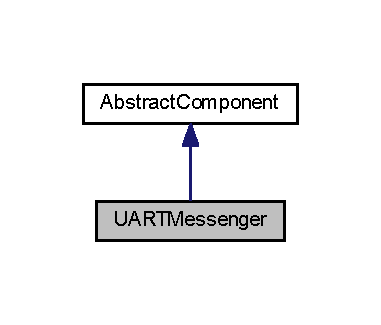
\includegraphics[width=183pt]{class_u_a_r_t_messenger__inherit__graph}
\end{center}
\end{figure}


Collaboration diagram for U\+A\+R\+T\+Messenger\+:\nopagebreak
\begin{figure}[H]
\begin{center}
\leavevmode
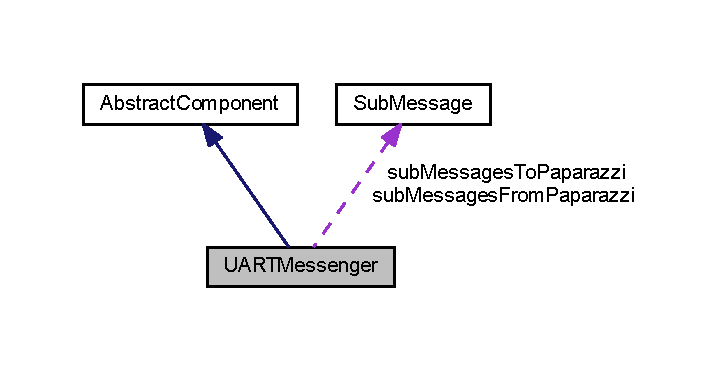
\includegraphics[width=346pt]{class_u_a_r_t_messenger__coll__graph}
\end{center}
\end{figure}
\subsection*{Public Member Functions}
\begin{DoxyCompactItemize}
\item 
\hyperlink{class_u_a_r_t_messenger_a2fcc2d4308e961996cf3dd120f297112}{U\+A\+R\+T\+Messenger} (Pin\+Name tx, Pin\+Name rx)
\begin{DoxyCompactList}\small\item\em Constructor for \hyperlink{class_u_a_r_t_messenger}{U\+A\+R\+T\+Messenger}. \end{DoxyCompactList}\item 
virtual void \hyperlink{class_u_a_r_t_messenger_a7f2c3bdcf3a2b082e52815b97be37281}{update} ()
\item 
void \hyperlink{class_u_a_r_t_messenger_ada0967869e320c236a211b405abf128a}{append\+Message} (const \hyperlink{struct_sub_message}{Sub\+Message} \&sub\+Message)
\begin{DoxyCompactList}\small\item\em Append new message for sending to Paparazzi. \end{DoxyCompactList}\item 
\hyperlink{struct_sub_message}{Sub\+Message} $\ast$ \hyperlink{class_u_a_r_t_messenger_affb33ad31e70001505e14d02e1f8a018}{check\+For\+Msg\+From\+Paparazzi} (int \hyperlink{class_abstract_component_a9c9c548149681b1a1dd935e66ed5dd11}{id})
\begin{DoxyCompactList}\small\item\em check if message from paparazzi has something for component with this id \end{DoxyCompactList}\item 
void \hyperlink{class_abstract_component_a58a59a9ea6c3b4c86fb3bf98ff1eaaef}{set\+Priority} (int p)
\begin{DoxyCompactList}\small\item\em Set priority to the component, used for updating order. \end{DoxyCompactList}\item 
int \hyperlink{class_abstract_component_ac0b440d1d642ff1292ec3c544d75a8f1}{get\+Priority} ()
\item 
bool \hyperlink{class_abstract_component_a0c2e458144111c5f599c66f168516abc}{operator$<$} (const \hyperlink{class_abstract_component}{Abstract\+Component} \&another) const
\begin{DoxyCompactList}\small\item\em Overloaded comparison operator \textquotesingle{}$<$\textquotesingle{}. \end{DoxyCompactList}\end{DoxyCompactItemize}
\subsection*{Protected Attributes}
\begin{DoxyCompactItemize}
\item 
int \hyperlink{class_abstract_component_a9c9c548149681b1a1dd935e66ed5dd11}{id}
\item 
int \hyperlink{class_abstract_component_aff57dfa5f31be093a06b55560e33fb95}{priority} = 0
\end{DoxyCompactItemize}
\subsection*{Static Protected Attributes}
\begin{DoxyCompactItemize}
\item 
static int \hyperlink{class_abstract_component_a99ce3e5fe7d73dac569b874c15fcaf0d}{s\+\_\+id} = 0
\begin{DoxyCompactList}\small\item\em The id for each component will be created in a sequence order staring with 1. \end{DoxyCompactList}\end{DoxyCompactItemize}
\subsection*{Private Member Functions}
\begin{DoxyCompactItemize}
\item 
bool \hyperlink{class_u_a_r_t_messenger_a8e90d75bc44daee10b5d6cf70e1c1fb4}{validate\+Checksum} (uint8\+\_\+t const $\ast$pkt, uint8\+\_\+t const length)
\begin{DoxyCompactList}\small\item\em Validate the checksum of the byte array. \end{DoxyCompactList}\item 
void \hyperlink{class_u_a_r_t_messenger_a21e6194acf3039eafdbb4e4c3b7876a3}{calculate\+Checksum} (uint8\+\_\+t $\ast$pkt, uint8\+\_\+t const length)
\begin{DoxyCompactList}\small\item\em Add checksum to the end of the byte array. \end{DoxyCompactList}\item 
void \hyperlink{class_u_a_r_t_messenger_a3ae1cd91810b34f89244cd157c436c3c}{process\+Paparazzi\+Msg} (int size)
\begin{DoxyCompactList}\small\item\em Process message from Paparazzi, if there is one. \end{DoxyCompactList}\item 
void \hyperlink{class_u_a_r_t_messenger_a91aa0a571db31d7a0a7f2535a97c30c3}{null\+Func} (int size)
\begin{DoxyCompactList}\small\item\em Used as null callback for mbed write() function. \end{DoxyCompactList}\end{DoxyCompactItemize}
\subsection*{Private Attributes}
\begin{DoxyCompactItemize}
\item 
Serial \hyperlink{class_u_a_r_t_messenger_aabc5283b509be4ce8335bbb2513e9b4c}{uart}
\item 
const \hyperlink{struct_sub_message}{Sub\+Message} $\ast$ \hyperlink{class_u_a_r_t_messenger_a1caaef4e6d8fa5005cd8ea5ff4937369}{sub\+Messages\+To\+Paparazzi} \mbox{[}\hyperlink{_u_a_r_t_messenger_8h_a6274d6c4801975be4baacd279386909d}{M\+A\+X\+\_\+\+M\+S\+G\+\_\+\+N\+U\+M\+B\+ER}\mbox{]}
\item 
\hyperlink{struct_sub_message}{Sub\+Message} \hyperlink{class_u_a_r_t_messenger_ad6fb0fea8b0262d46cc97f5d5b262a51}{sub\+Messages\+From\+Paparazzi} \mbox{[}\hyperlink{_u_a_r_t_messenger_8h_a6274d6c4801975be4baacd279386909d}{M\+A\+X\+\_\+\+M\+S\+G\+\_\+\+N\+U\+M\+B\+ER}\mbox{]}
\item 
uint8\+\_\+t \hyperlink{class_u_a_r_t_messenger_ae47f334cdd266ae4cde0715154f0ace3}{to\+Paparazzi\+Count}
\item 
uint8\+\_\+t \hyperlink{class_u_a_r_t_messenger_a72ecf1c51d6a28c582fff9fd454145dd}{from\+Paparazzi\+Count}
\item 
uint8\+\_\+t \hyperlink{class_u_a_r_t_messenger_ae2a77be89a1f84b466eab4753929b902}{to\+Paparazzi\+Msg\+Length}
\item 
uint8\+\_\+t \hyperlink{class_u_a_r_t_messenger_ad564c1e74510c03c7cb4ec5b7c57a802}{to\+Paparazzi\+Msg} \mbox{[}\hyperlink{_u_a_r_t_messenger_8h_a6821bafc3c88dfb2e433a095df9940c6}{B\+U\+F\+\_\+\+S\+I\+ZE}\mbox{]}
\item 
uint8\+\_\+t \hyperlink{class_u_a_r_t_messenger_a0cdc15059654a4231fcfe312612c73f3}{from\+Paparazzi\+Msg} \mbox{[}\hyperlink{_u_a_r_t_messenger_8h_a6821bafc3c88dfb2e433a095df9940c6}{B\+U\+F\+\_\+\+S\+I\+ZE}\mbox{]}
\item 
uint8\+\_\+t \hyperlink{class_u_a_r_t_messenger_abfc75506508a4d627236fc61f0f536b2}{start\+Byte}
\item 
uint8\+\_\+t \hyperlink{class_u_a_r_t_messenger_abd1f0ee480db317c51ea633fff5dd9af}{stop\+Byte}
\end{DoxyCompactItemize}


\subsection{Detailed Description}


Definition at line 10 of file U\+A\+R\+T\+Messenger.\+h.



\subsection{Constructor \& Destructor Documentation}
\mbox{\Hypertarget{class_u_a_r_t_messenger_a2fcc2d4308e961996cf3dd120f297112}\label{class_u_a_r_t_messenger_a2fcc2d4308e961996cf3dd120f297112}} 
\index{U\+A\+R\+T\+Messenger@{U\+A\+R\+T\+Messenger}!U\+A\+R\+T\+Messenger@{U\+A\+R\+T\+Messenger}}
\index{U\+A\+R\+T\+Messenger@{U\+A\+R\+T\+Messenger}!U\+A\+R\+T\+Messenger@{U\+A\+R\+T\+Messenger}}
\subsubsection{\texorpdfstring{U\+A\+R\+T\+Messenger()}{UARTMessenger()}}
{\footnotesize\ttfamily U\+A\+R\+T\+Messenger\+::\+U\+A\+R\+T\+Messenger (\begin{DoxyParamCaption}\item[{Pin\+Name}]{tx,  }\item[{Pin\+Name}]{rx }\end{DoxyParamCaption})}



Constructor for \hyperlink{class_u_a_r_t_messenger}{U\+A\+R\+T\+Messenger}. 


\begin{DoxyParams}{Parameters}
{\em tx} & transmit pin \\
\hline
{\em rx} & receive pin \\
\hline
\end{DoxyParams}


Definition at line 8 of file U\+A\+R\+T\+Messenger.\+cpp.


\begin{DoxyCode}
8                                                    : \hyperlink{class_u_a_r_t_messenger_aabc5283b509be4ce8335bbb2513e9b4c}{uart}(tx, rx, 9600) \{
9     \textcolor{keywordtype}{id} = ++\hyperlink{class_abstract_component_a99ce3e5fe7d73dac569b874c15fcaf0d}{s\_id};
10 
11     \hyperlink{class_u_a_r_t_messenger_ae47f334cdd266ae4cde0715154f0ace3}{toPaparazziCount} = 0;
12     \hyperlink{class_u_a_r_t_messenger_a72ecf1c51d6a28c582fff9fd454145dd}{fromPaparazziCount} = 0;
13     \hyperlink{class_u_a_r_t_messenger_ae2a77be89a1f84b466eab4753929b902}{toPaparazziMsgLength} = \hyperlink{_u_a_r_t_messenger_8h_a03caf75f3be11c473c11ea925cef73e2}{MIN\_MSG\_SIZE};
14 
15     \hyperlink{class_u_a_r_t_messenger_abfc75506508a4d627236fc61f0f536b2}{startByte} = 0xFE;
16     \hyperlink{class_u_a_r_t_messenger_abd1f0ee480db317c51ea633fff5dd9af}{stopByte} = 0xFF;
17 \}
\end{DoxyCode}


\subsection{Member Function Documentation}
\mbox{\Hypertarget{class_u_a_r_t_messenger_ada0967869e320c236a211b405abf128a}\label{class_u_a_r_t_messenger_ada0967869e320c236a211b405abf128a}} 
\index{U\+A\+R\+T\+Messenger@{U\+A\+R\+T\+Messenger}!append\+Message@{append\+Message}}
\index{append\+Message@{append\+Message}!U\+A\+R\+T\+Messenger@{U\+A\+R\+T\+Messenger}}
\subsubsection{\texorpdfstring{append\+Message()}{appendMessage()}}
{\footnotesize\ttfamily void U\+A\+R\+T\+Messenger\+::append\+Message (\begin{DoxyParamCaption}\item[{const \hyperlink{struct_sub_message}{Sub\+Message} \&}]{sub\+Message }\end{DoxyParamCaption})}



Append new message for sending to Paparazzi. 


\begin{DoxyParams}{Parameters}
{\em sub\+Message} & message to be added \\
\hline
\end{DoxyParams}


Definition at line 56 of file U\+A\+R\+T\+Messenger.\+cpp.


\begin{DoxyCode}
56                                                               \{
57     \hyperlink{class_i_r_q_lock}{IRQLock} lock;
58     \textcolor{keywordflow}{if} (\hyperlink{class_u_a_r_t_messenger_ae47f334cdd266ae4cde0715154f0ace3}{toPaparazziCount} >= \hyperlink{_u_a_r_t_messenger_8h_a6274d6c4801975be4baacd279386909d}{MAX\_MSG\_NUMBER}) \{
59         \textcolor{keywordflow}{return};
60     \}
61     \hyperlink{class_u_a_r_t_messenger_a1caaef4e6d8fa5005cd8ea5ff4937369}{subMessagesToPaparazzi}[\hyperlink{class_u_a_r_t_messenger_ae47f334cdd266ae4cde0715154f0ace3}{toPaparazziCount}] = &subMessage;
62     \hyperlink{class_u_a_r_t_messenger_ae2a77be89a1f84b466eab4753929b902}{toPaparazziMsgLength} += \hyperlink{class_u_a_r_t_messenger_a1caaef4e6d8fa5005cd8ea5ff4937369}{subMessagesToPaparazzi}[
      \hyperlink{class_u_a_r_t_messenger_ae47f334cdd266ae4cde0715154f0ace3}{toPaparazziCount}]->\hyperlink{struct_sub_message_a276e06f5335ca7857c21ac8c0e51bd6d}{length} + 3;
63     \hyperlink{class_u_a_r_t_messenger_ae47f334cdd266ae4cde0715154f0ace3}{toPaparazziCount}++;
64 \}
\end{DoxyCode}
Here is the caller graph for this function\+:\nopagebreak
\begin{figure}[H]
\begin{center}
\leavevmode
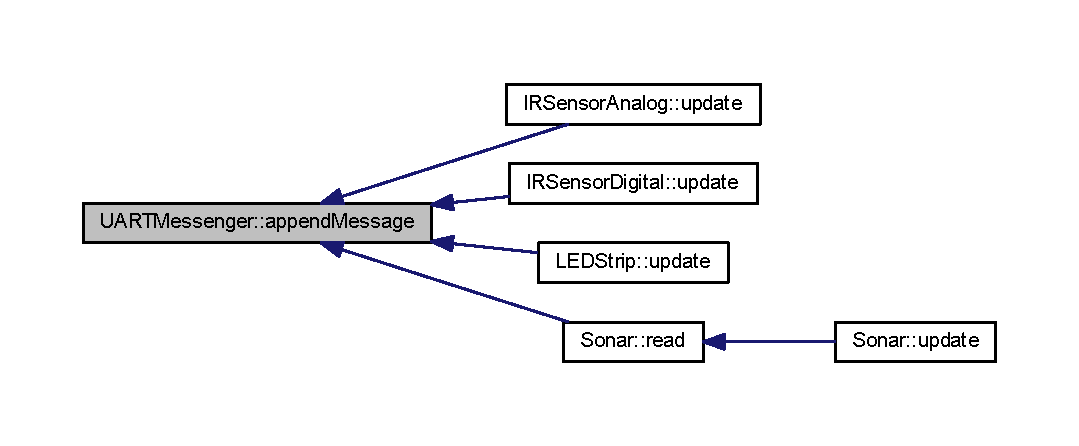
\includegraphics[width=350pt]{class_u_a_r_t_messenger_ada0967869e320c236a211b405abf128a_icgraph}
\end{center}
\end{figure}
\mbox{\Hypertarget{class_u_a_r_t_messenger_a21e6194acf3039eafdbb4e4c3b7876a3}\label{class_u_a_r_t_messenger_a21e6194acf3039eafdbb4e4c3b7876a3}} 
\index{U\+A\+R\+T\+Messenger@{U\+A\+R\+T\+Messenger}!calculate\+Checksum@{calculate\+Checksum}}
\index{calculate\+Checksum@{calculate\+Checksum}!U\+A\+R\+T\+Messenger@{U\+A\+R\+T\+Messenger}}
\subsubsection{\texorpdfstring{calculate\+Checksum()}{calculateChecksum()}}
{\footnotesize\ttfamily void U\+A\+R\+T\+Messenger\+::calculate\+Checksum (\begin{DoxyParamCaption}\item[{uint8\+\_\+t $\ast$}]{pkt,  }\item[{uint8\+\_\+t const}]{length }\end{DoxyParamCaption})\hspace{0.3cm}{\ttfamily [private]}}



Add checksum to the end of the byte array. 


\begin{DoxyParams}{Parameters}
{\em pkt} & pointer to the byte array \\
\hline
{\em length} & number of bytes in the array \\
\hline
\end{DoxyParams}


Definition at line 83 of file U\+A\+R\+T\+Messenger.\+cpp.


\begin{DoxyCode}
83                                                                         \{
84     uint8\_t pos = 0;
85     uint8\_t sum = 0;
86     \textcolor{keywordflow}{while} (pos < (length - 1)) \{
87         sum += *(pkt + pos++);
88     \}
89     \textcolor{comment}{// put the checksum into the data stream}
90     *(pkt + pos) = 0x0 - sum;
91 \}
\end{DoxyCode}
Here is the caller graph for this function\+:\nopagebreak
\begin{figure}[H]
\begin{center}
\leavevmode
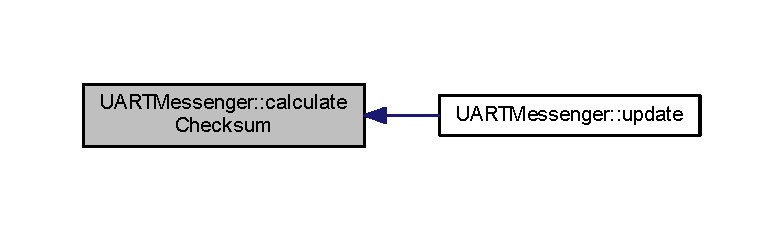
\includegraphics[width=350pt]{class_u_a_r_t_messenger_a21e6194acf3039eafdbb4e4c3b7876a3_icgraph}
\end{center}
\end{figure}
\mbox{\Hypertarget{class_u_a_r_t_messenger_affb33ad31e70001505e14d02e1f8a018}\label{class_u_a_r_t_messenger_affb33ad31e70001505e14d02e1f8a018}} 
\index{U\+A\+R\+T\+Messenger@{U\+A\+R\+T\+Messenger}!check\+For\+Msg\+From\+Paparazzi@{check\+For\+Msg\+From\+Paparazzi}}
\index{check\+For\+Msg\+From\+Paparazzi@{check\+For\+Msg\+From\+Paparazzi}!U\+A\+R\+T\+Messenger@{U\+A\+R\+T\+Messenger}}
\subsubsection{\texorpdfstring{check\+For\+Msg\+From\+Paparazzi()}{checkForMsgFromPaparazzi()}}
{\footnotesize\ttfamily \hyperlink{struct_sub_message}{Sub\+Message} $\ast$ U\+A\+R\+T\+Messenger\+::check\+For\+Msg\+From\+Paparazzi (\begin{DoxyParamCaption}\item[{int}]{id }\end{DoxyParamCaption})}



check if message from paparazzi has something for component with this id 


\begin{DoxyParams}{Parameters}
{\em id} & -\/ id of the component \\
\hline
\end{DoxyParams}
\begin{DoxyReturn}{Returns}
Sub\+Message$\ast$ if found, nullptr otherwise 
\end{DoxyReturn}


Definition at line 130 of file U\+A\+R\+T\+Messenger.\+cpp.


\begin{DoxyCode}
130                                                           \{
131     \textcolor{comment}{// check if message from paparazzi has something for component with this id}
132     \textcolor{keywordflow}{for} (\textcolor{keywordtype}{int} i = 0; i < \hyperlink{class_u_a_r_t_messenger_a72ecf1c51d6a28c582fff9fd454145dd}{fromPaparazziCount}; i++) \{
133         \textcolor{keywordflow}{if} (\hyperlink{class_u_a_r_t_messenger_ad6fb0fea8b0262d46cc97f5d5b262a51}{subMessagesFromPaparazzi}[i].\textcolor{keywordtype}{id} == \textcolor{keywordtype}{id}) \{
134             \hyperlink{class_u_a_r_t_messenger_ad6fb0fea8b0262d46cc97f5d5b262a51}{subMessagesFromPaparazzi}[i].\hyperlink{struct_sub_message_af3acc450c0686d7a9d15ccd9d548cb6d}{id} = 0; \textcolor{comment}{// invalidate this submessage}
135             \textcolor{keywordflow}{return} &\hyperlink{class_u_a_r_t_messenger_ad6fb0fea8b0262d46cc97f5d5b262a51}{subMessagesFromPaparazzi}[i];
136         \}
137     \}
138     \textcolor{keywordflow}{return} \textcolor{keyword}{nullptr};
139 \}
\end{DoxyCode}
Here is the caller graph for this function\+:\nopagebreak
\begin{figure}[H]
\begin{center}
\leavevmode
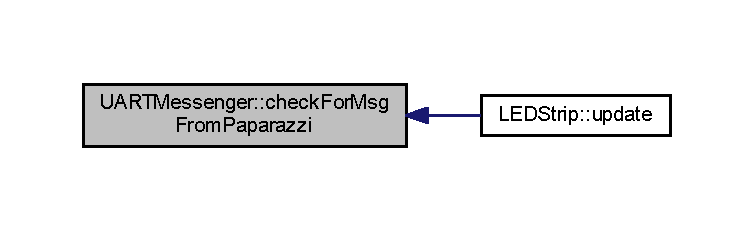
\includegraphics[width=350pt]{class_u_a_r_t_messenger_affb33ad31e70001505e14d02e1f8a018_icgraph}
\end{center}
\end{figure}
\mbox{\Hypertarget{class_abstract_component_ac0b440d1d642ff1292ec3c544d75a8f1}\label{class_abstract_component_ac0b440d1d642ff1292ec3c544d75a8f1}} 
\index{U\+A\+R\+T\+Messenger@{U\+A\+R\+T\+Messenger}!get\+Priority@{get\+Priority}}
\index{get\+Priority@{get\+Priority}!U\+A\+R\+T\+Messenger@{U\+A\+R\+T\+Messenger}}
\subsubsection{\texorpdfstring{get\+Priority()}{getPriority()}}
{\footnotesize\ttfamily int Abstract\+Component\+::get\+Priority (\begin{DoxyParamCaption}{ }\end{DoxyParamCaption})\hspace{0.3cm}{\ttfamily [inline]}, {\ttfamily [inherited]}}

\begin{DoxyReturn}{Returns}
priority of the component 
\end{DoxyReturn}


Definition at line 25 of file Abstract\+Component.\+h.


\begin{DoxyCode}
25                       \{
26         \textcolor{keywordflow}{return} \hyperlink{class_abstract_component_aff57dfa5f31be093a06b55560e33fb95}{priority};
27     \}
\end{DoxyCode}
Here is the call graph for this function\+:
\nopagebreak
\begin{figure}[H]
\begin{center}
\leavevmode
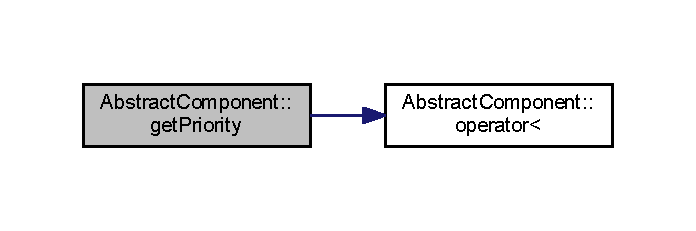
\includegraphics[width=334pt]{class_abstract_component_ac0b440d1d642ff1292ec3c544d75a8f1_cgraph}
\end{center}
\end{figure}
\mbox{\Hypertarget{class_u_a_r_t_messenger_a91aa0a571db31d7a0a7f2535a97c30c3}\label{class_u_a_r_t_messenger_a91aa0a571db31d7a0a7f2535a97c30c3}} 
\index{U\+A\+R\+T\+Messenger@{U\+A\+R\+T\+Messenger}!null\+Func@{null\+Func}}
\index{null\+Func@{null\+Func}!U\+A\+R\+T\+Messenger@{U\+A\+R\+T\+Messenger}}
\subsubsection{\texorpdfstring{null\+Func()}{nullFunc()}}
{\footnotesize\ttfamily void U\+A\+R\+T\+Messenger\+::null\+Func (\begin{DoxyParamCaption}\item[{int}]{size }\end{DoxyParamCaption})\hspace{0.3cm}{\ttfamily [private]}}



Used as null callback for mbed write() function. 


\begin{DoxyParams}{Parameters}
{\em size} & -\/ size of the message \\
\hline
\end{DoxyParams}


Definition at line 125 of file U\+A\+R\+T\+Messenger.\+cpp.


\begin{DoxyCode}
125 \{\}
\end{DoxyCode}
Here is the caller graph for this function\+:\nopagebreak
\begin{figure}[H]
\begin{center}
\leavevmode
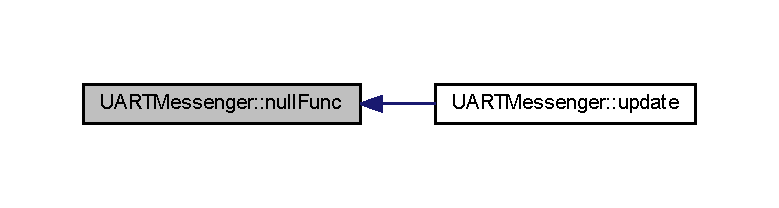
\includegraphics[width=350pt]{class_u_a_r_t_messenger_a91aa0a571db31d7a0a7f2535a97c30c3_icgraph}
\end{center}
\end{figure}
\mbox{\Hypertarget{class_abstract_component_a0c2e458144111c5f599c66f168516abc}\label{class_abstract_component_a0c2e458144111c5f599c66f168516abc}} 
\index{U\+A\+R\+T\+Messenger@{U\+A\+R\+T\+Messenger}!operator$<$@{operator$<$}}
\index{operator$<$@{operator$<$}!U\+A\+R\+T\+Messenger@{U\+A\+R\+T\+Messenger}}
\subsubsection{\texorpdfstring{operator$<$()}{operator<()}}
{\footnotesize\ttfamily bool Abstract\+Component\+::operator$<$ (\begin{DoxyParamCaption}\item[{const \hyperlink{class_abstract_component}{Abstract\+Component} \&}]{another }\end{DoxyParamCaption}) const\hspace{0.3cm}{\ttfamily [inherited]}}



Overloaded comparison operator \textquotesingle{}$<$\textquotesingle{}. 


\begin{DoxyParams}{Parameters}
{\em another} & component for comparison \\
\hline
\end{DoxyParams}
\begin{DoxyReturn}{Returns}
true if id is smaller then the id of another component 
\end{DoxyReturn}


Definition at line 8 of file Abstract\+Component.\+cpp.


\begin{DoxyCode}
8                                                                         \{
9     \textcolor{keywordflow}{return} \textcolor{keywordtype}{id} < another.\hyperlink{class_abstract_component_a9c9c548149681b1a1dd935e66ed5dd11}{id};
10 \}
\end{DoxyCode}
Here is the caller graph for this function\+:
\nopagebreak
\begin{figure}[H]
\begin{center}
\leavevmode
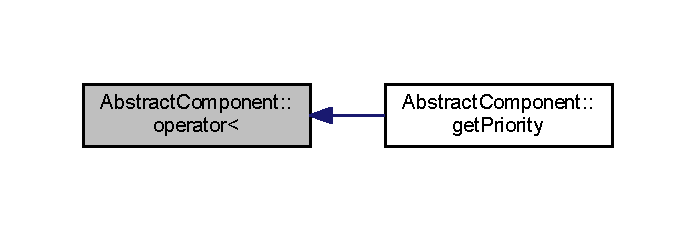
\includegraphics[width=334pt]{class_abstract_component_a0c2e458144111c5f599c66f168516abc_icgraph}
\end{center}
\end{figure}
\mbox{\Hypertarget{class_u_a_r_t_messenger_a3ae1cd91810b34f89244cd157c436c3c}\label{class_u_a_r_t_messenger_a3ae1cd91810b34f89244cd157c436c3c}} 
\index{U\+A\+R\+T\+Messenger@{U\+A\+R\+T\+Messenger}!process\+Paparazzi\+Msg@{process\+Paparazzi\+Msg}}
\index{process\+Paparazzi\+Msg@{process\+Paparazzi\+Msg}!U\+A\+R\+T\+Messenger@{U\+A\+R\+T\+Messenger}}
\subsubsection{\texorpdfstring{process\+Paparazzi\+Msg()}{processPaparazziMsg()}}
{\footnotesize\ttfamily void U\+A\+R\+T\+Messenger\+::process\+Paparazzi\+Msg (\begin{DoxyParamCaption}\item[{int}]{size }\end{DoxyParamCaption})\hspace{0.3cm}{\ttfamily [private]}}



Process message from Paparazzi, if there is one. 


\begin{DoxyParams}{Parameters}
{\em size} & -\/ size of the message\\
\hline
\end{DoxyParams}
Used as callback for mbed read() function. 

Definition at line 97 of file U\+A\+R\+T\+Messenger.\+cpp.


\begin{DoxyCode}
97                                                 \{
98     \textcolor{keywordtype}{bool} validation = \hyperlink{class_u_a_r_t_messenger_a8e90d75bc44daee10b5d6cf70e1c1fb4}{validateChecksum}(\hyperlink{class_u_a_r_t_messenger_a0cdc15059654a4231fcfe312612c73f3}{fromPaparazziMsg}, size);
99 
100     \textcolor{comment}{// ATTENTION: change to 'if (validation)' in real application}
101     \textcolor{keywordflow}{if} (\textcolor{keyword}{true}) \{
102         \textcolor{comment}{// Currently it's just overwriting the old messages}
103         \hyperlink{class_u_a_r_t_messenger_a72ecf1c51d6a28c582fff9fd454145dd}{fromPaparazziCount} = \hyperlink{class_u_a_r_t_messenger_a0cdc15059654a4231fcfe312612c73f3}{fromPaparazziMsg}[0];
104 
105         \textcolor{keywordtype}{int} pos = 1;
106         \textcolor{keywordflow}{for}(\textcolor{keywordtype}{int} i = 0; i < \hyperlink{class_u_a_r_t_messenger_a72ecf1c51d6a28c582fff9fd454145dd}{fromPaparazziCount} && i < 
      \hyperlink{_u_a_r_t_messenger_8h_a6274d6c4801975be4baacd279386909d}{MAX\_MSG\_NUMBER}; i++) \{
107             \hyperlink{struct_sub_message}{SubMessage} paparazziSubMessage;
108 
109             paparazziSubMessage.\hyperlink{struct_sub_message_a064f1d26d553da776dc749d37a18a499}{type} = \hyperlink{class_u_a_r_t_messenger_a0cdc15059654a4231fcfe312612c73f3}{fromPaparazziMsg}[pos++];
110             paparazziSubMessage.\hyperlink{struct_sub_message_af3acc450c0686d7a9d15ccd9d548cb6d}{id} = \hyperlink{class_u_a_r_t_messenger_a0cdc15059654a4231fcfe312612c73f3}{fromPaparazziMsg}[pos++];
111             paparazziSubMessage.\hyperlink{struct_sub_message_a276e06f5335ca7857c21ac8c0e51bd6d}{length} = \hyperlink{class_u_a_r_t_messenger_a0cdc15059654a4231fcfe312612c73f3}{fromPaparazziMsg}[pos++];
112 
113             \textcolor{keywordflow}{for} (\textcolor{keywordtype}{int} j = 0; j < paparazziSubMessage.\hyperlink{struct_sub_message_a276e06f5335ca7857c21ac8c0e51bd6d}{length}; j++) \{
114                 paparazziSubMessage.\hyperlink{struct_sub_message_a7d923c5cdaa380c27d7c4cf60ea7c1be}{data}[j] = \hyperlink{class_u_a_r_t_messenger_a0cdc15059654a4231fcfe312612c73f3}{fromPaparazziMsg}[pos++];
115             \}
116 
117             \hyperlink{class_u_a_r_t_messenger_ad6fb0fea8b0262d46cc97f5d5b262a51}{subMessagesFromPaparazzi}[i] = paparazziSubMessage;
118         \}
119     \}
120 \}
\end{DoxyCode}
Here is the call graph for this function\+:\nopagebreak
\begin{figure}[H]
\begin{center}
\leavevmode
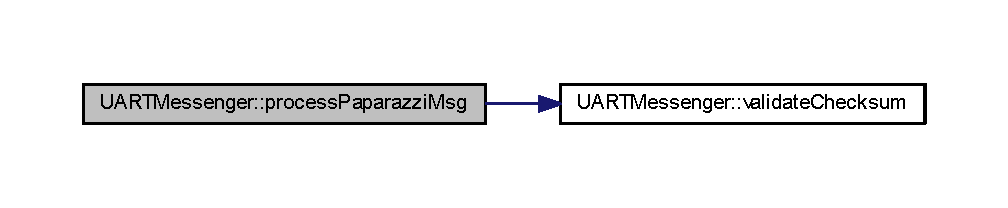
\includegraphics[width=350pt]{class_u_a_r_t_messenger_a3ae1cd91810b34f89244cd157c436c3c_cgraph}
\end{center}
\end{figure}
Here is the caller graph for this function\+:\nopagebreak
\begin{figure}[H]
\begin{center}
\leavevmode
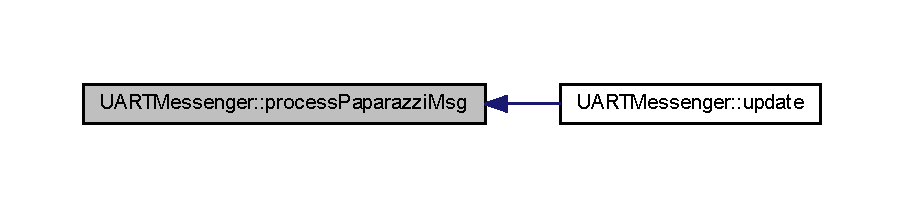
\includegraphics[width=350pt]{class_u_a_r_t_messenger_a3ae1cd91810b34f89244cd157c436c3c_icgraph}
\end{center}
\end{figure}
\mbox{\Hypertarget{class_abstract_component_a58a59a9ea6c3b4c86fb3bf98ff1eaaef}\label{class_abstract_component_a58a59a9ea6c3b4c86fb3bf98ff1eaaef}} 
\index{U\+A\+R\+T\+Messenger@{U\+A\+R\+T\+Messenger}!set\+Priority@{set\+Priority}}
\index{set\+Priority@{set\+Priority}!U\+A\+R\+T\+Messenger@{U\+A\+R\+T\+Messenger}}
\subsubsection{\texorpdfstring{set\+Priority()}{setPriority()}}
{\footnotesize\ttfamily void Abstract\+Component\+::set\+Priority (\begin{DoxyParamCaption}\item[{int}]{p }\end{DoxyParamCaption})\hspace{0.3cm}{\ttfamily [inline]}, {\ttfamily [inherited]}}



Set priority to the component, used for updating order. 


\begin{DoxyParams}{Parameters}
{\em p} & priority \\
\hline
\end{DoxyParams}


Definition at line 18 of file Abstract\+Component.\+h.


\begin{DoxyCode}
18                             \{
19         \hyperlink{class_abstract_component_aff57dfa5f31be093a06b55560e33fb95}{priority} = p;
20     \}
\end{DoxyCode}
\mbox{\Hypertarget{class_u_a_r_t_messenger_a7f2c3bdcf3a2b082e52815b97be37281}\label{class_u_a_r_t_messenger_a7f2c3bdcf3a2b082e52815b97be37281}} 
\index{U\+A\+R\+T\+Messenger@{U\+A\+R\+T\+Messenger}!update@{update}}
\index{update@{update}!U\+A\+R\+T\+Messenger@{U\+A\+R\+T\+Messenger}}
\subsubsection{\texorpdfstring{update()}{update()}}
{\footnotesize\ttfamily void U\+A\+R\+T\+Messenger\+::update (\begin{DoxyParamCaption}{ }\end{DoxyParamCaption})\hspace{0.3cm}{\ttfamily [virtual]}}



Implements \hyperlink{class_abstract_component_af25a90b8ab213762221c3b358d9873f3}{Abstract\+Component}.



Definition at line 19 of file U\+A\+R\+T\+Messenger.\+cpp.


\begin{DoxyCode}
19                            \{
20     \hyperlink{class_i_r_q_lock}{IRQLock} lock;
21 
22     memset(\hyperlink{class_u_a_r_t_messenger_ad564c1e74510c03c7cb4ec5b7c57a802}{toPaparazziMsg}, 0, \hyperlink{_u_a_r_t_messenger_8h_a6821bafc3c88dfb2e433a095df9940c6}{BUF\_SIZE});
23 
24     \hyperlink{class_u_a_r_t_messenger_ad564c1e74510c03c7cb4ec5b7c57a802}{toPaparazziMsg}[0] = \hyperlink{class_u_a_r_t_messenger_ae47f334cdd266ae4cde0715154f0ace3}{toPaparazziCount};
25 
26     \textcolor{comment}{// add current submessages}
27     \textcolor{keywordtype}{int} pos = 0;
28     \textcolor{keywordflow}{for} (\textcolor{keywordtype}{int} i = 0; i < \hyperlink{class_u_a_r_t_messenger_ae47f334cdd266ae4cde0715154f0ace3}{toPaparazziCount}; i++) \{
29         \hyperlink{class_u_a_r_t_messenger_ad564c1e74510c03c7cb4ec5b7c57a802}{toPaparazziMsg}[++pos] = \hyperlink{class_u_a_r_t_messenger_a1caaef4e6d8fa5005cd8ea5ff4937369}{subMessagesToPaparazzi}[i]->
      \hyperlink{struct_sub_message_af3acc450c0686d7a9d15ccd9d548cb6d}{id};
30         \hyperlink{class_u_a_r_t_messenger_ad564c1e74510c03c7cb4ec5b7c57a802}{toPaparazziMsg}[++pos] = \hyperlink{class_u_a_r_t_messenger_a1caaef4e6d8fa5005cd8ea5ff4937369}{subMessagesToPaparazzi}[i]->
      \hyperlink{struct_sub_message_a064f1d26d553da776dc749d37a18a499}{type};
31         \hyperlink{class_u_a_r_t_messenger_ad564c1e74510c03c7cb4ec5b7c57a802}{toPaparazziMsg}[++pos] = \hyperlink{class_u_a_r_t_messenger_a1caaef4e6d8fa5005cd8ea5ff4937369}{subMessagesToPaparazzi}[i]->
      \hyperlink{struct_sub_message_a276e06f5335ca7857c21ac8c0e51bd6d}{length};
32         \textcolor{keywordflow}{for} (\textcolor{keywordtype}{int} j = 0; j < \hyperlink{class_u_a_r_t_messenger_a1caaef4e6d8fa5005cd8ea5ff4937369}{subMessagesToPaparazzi}[i]->
      \hyperlink{struct_sub_message_a276e06f5335ca7857c21ac8c0e51bd6d}{length}; j++) \{
33             \hyperlink{class_u_a_r_t_messenger_ad564c1e74510c03c7cb4ec5b7c57a802}{toPaparazziMsg}[++pos] = \hyperlink{class_u_a_r_t_messenger_a1caaef4e6d8fa5005cd8ea5ff4937369}{subMessagesToPaparazzi}[i]->
      \hyperlink{struct_sub_message_a7d923c5cdaa380c27d7c4cf60ea7c1be}{data}[j];
34         \}
35     \}
36 
37     \hyperlink{class_u_a_r_t_messenger_a21e6194acf3039eafdbb4e4c3b7876a3}{calculateChecksum}(\hyperlink{class_u_a_r_t_messenger_ad564c1e74510c03c7cb4ec5b7c57a802}{toPaparazziMsg}, 
      \hyperlink{class_u_a_r_t_messenger_ae2a77be89a1f84b466eab4753929b902}{toPaparazziMsgLength});
38 
39     \textcolor{comment}{// send the message via UART}
40     \hyperlink{class_u_a_r_t_messenger_aabc5283b509be4ce8335bbb2513e9b4c}{uart}.write(\hyperlink{class_u_a_r_t_messenger_ad564c1e74510c03c7cb4ec5b7c57a802}{toPaparazziMsg}, \hyperlink{class_u_a_r_t_messenger_ae2a77be89a1f84b466eab4753929b902}{toPaparazziMsgLength}, callback(\textcolor{keyword}{this}, &
      \hyperlink{class_u_a_r_t_messenger_a91aa0a571db31d7a0a7f2535a97c30c3}{UARTMessenger::nullFunc}));
41 
42     \textcolor{comment}{// forget old messages from Paparazzi}
43     memset(\hyperlink{class_u_a_r_t_messenger_a0cdc15059654a4231fcfe312612c73f3}{fromPaparazziMsg}, 0, \hyperlink{_u_a_r_t_messenger_8h_a6821bafc3c88dfb2e433a095df9940c6}{BUF\_SIZE});
44 
45     \textcolor{comment}{// check if we have message from Paparazzi}
46     \hyperlink{class_u_a_r_t_messenger_aabc5283b509be4ce8335bbb2513e9b4c}{uart}.read(\hyperlink{class_u_a_r_t_messenger_a0cdc15059654a4231fcfe312612c73f3}{fromPaparazziMsg}, \hyperlink{_u_a_r_t_messenger_8h_a6821bafc3c88dfb2e433a095df9940c6}{BUF\_SIZE}, callback(\textcolor{keyword}{this}, &
      \hyperlink{class_u_a_r_t_messenger_a3ae1cd91810b34f89244cd157c436c3c}{UARTMessenger::processPaparazziMsg}), SERIAL\_EVENT\_RX\_COMPLETE | 
      SERIAL\_EVENT\_RX\_CHARACTER\_MATCH, \hyperlink{class_u_a_r_t_messenger_abd1f0ee480db317c51ea633fff5dd9af}{stopByte});
47 
48     \textcolor{comment}{// forget about old messages to Paparazzi}
49     toPaparazziCount = 0;
50     \hyperlink{class_u_a_r_t_messenger_ae2a77be89a1f84b466eab4753929b902}{toPaparazziMsgLength} = \hyperlink{_u_a_r_t_messenger_8h_a03caf75f3be11c473c11ea925cef73e2}{MIN\_MSG\_SIZE};
51 \}
\end{DoxyCode}
Here is the call graph for this function\+:\nopagebreak
\begin{figure}[H]
\begin{center}
\leavevmode
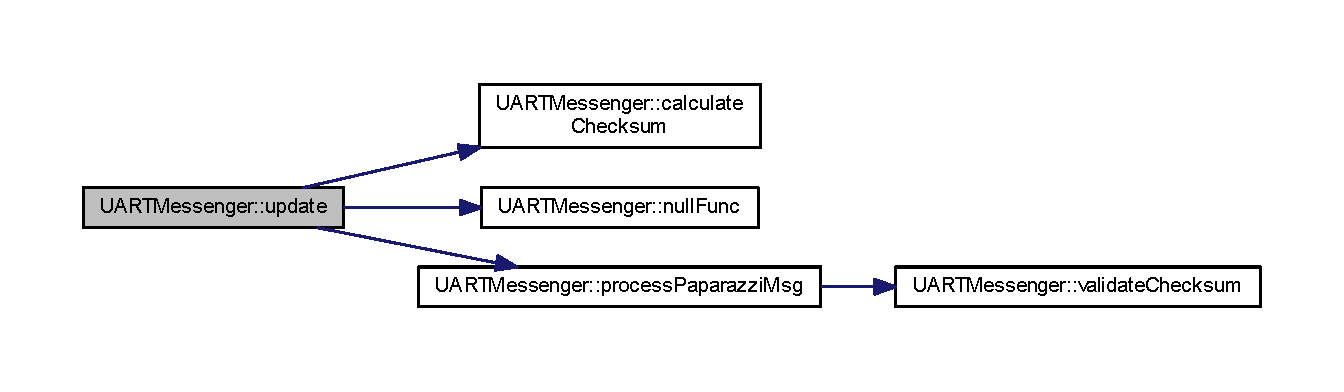
\includegraphics[width=350pt]{class_u_a_r_t_messenger_a7f2c3bdcf3a2b082e52815b97be37281_cgraph}
\end{center}
\end{figure}
\mbox{\Hypertarget{class_u_a_r_t_messenger_a8e90d75bc44daee10b5d6cf70e1c1fb4}\label{class_u_a_r_t_messenger_a8e90d75bc44daee10b5d6cf70e1c1fb4}} 
\index{U\+A\+R\+T\+Messenger@{U\+A\+R\+T\+Messenger}!validate\+Checksum@{validate\+Checksum}}
\index{validate\+Checksum@{validate\+Checksum}!U\+A\+R\+T\+Messenger@{U\+A\+R\+T\+Messenger}}
\subsubsection{\texorpdfstring{validate\+Checksum()}{validateChecksum()}}
{\footnotesize\ttfamily bool U\+A\+R\+T\+Messenger\+::validate\+Checksum (\begin{DoxyParamCaption}\item[{uint8\+\_\+t const $\ast$}]{pkt,  }\item[{uint8\+\_\+t const}]{length }\end{DoxyParamCaption})\hspace{0.3cm}{\ttfamily [private]}}



Validate the checksum of the byte array. 


\begin{DoxyParams}{Parameters}
{\em pkt} & pointer to the byte array \\
\hline
{\em length} & number of bytes in the array\\
\hline
\end{DoxyParams}
\begin{DoxyReturn}{Returns}
true if validation was successful 
\end{DoxyReturn}


Definition at line 69 of file U\+A\+R\+T\+Messenger.\+cpp.


\begin{DoxyCode}
69                                                                              \{
70     uint8\_t pos = 0;
71     uint8\_t sum = 0;
72     \textcolor{keywordflow}{while} (pos < (length - 1)) \{
73         sum += *(pkt + pos++);
74     \}
75     sum = 0x0 - sum;
76 
77     \textcolor{keywordflow}{return} (sum == *(pkt + pos));
78 \}
\end{DoxyCode}
Here is the caller graph for this function\+:\nopagebreak
\begin{figure}[H]
\begin{center}
\leavevmode
\includegraphics[width=350pt]{class_u_a_r_t_messenger_a8e90d75bc44daee10b5d6cf70e1c1fb4_icgraph}
\end{center}
\end{figure}


\subsection{Member Data Documentation}
\mbox{\Hypertarget{class_u_a_r_t_messenger_a72ecf1c51d6a28c582fff9fd454145dd}\label{class_u_a_r_t_messenger_a72ecf1c51d6a28c582fff9fd454145dd}} 
\index{U\+A\+R\+T\+Messenger@{U\+A\+R\+T\+Messenger}!from\+Paparazzi\+Count@{from\+Paparazzi\+Count}}
\index{from\+Paparazzi\+Count@{from\+Paparazzi\+Count}!U\+A\+R\+T\+Messenger@{U\+A\+R\+T\+Messenger}}
\subsubsection{\texorpdfstring{from\+Paparazzi\+Count}{fromPaparazziCount}}
{\footnotesize\ttfamily uint8\+\_\+t U\+A\+R\+T\+Messenger\+::from\+Paparazzi\+Count\hspace{0.3cm}{\ttfamily [private]}}



Definition at line 61 of file U\+A\+R\+T\+Messenger.\+h.

\mbox{\Hypertarget{class_u_a_r_t_messenger_a0cdc15059654a4231fcfe312612c73f3}\label{class_u_a_r_t_messenger_a0cdc15059654a4231fcfe312612c73f3}} 
\index{U\+A\+R\+T\+Messenger@{U\+A\+R\+T\+Messenger}!from\+Paparazzi\+Msg@{from\+Paparazzi\+Msg}}
\index{from\+Paparazzi\+Msg@{from\+Paparazzi\+Msg}!U\+A\+R\+T\+Messenger@{U\+A\+R\+T\+Messenger}}
\subsubsection{\texorpdfstring{from\+Paparazzi\+Msg}{fromPaparazziMsg}}
{\footnotesize\ttfamily uint8\+\_\+t U\+A\+R\+T\+Messenger\+::from\+Paparazzi\+Msg\mbox{[}\hyperlink{_u_a_r_t_messenger_8h_a6821bafc3c88dfb2e433a095df9940c6}{B\+U\+F\+\_\+\+S\+I\+ZE}\mbox{]}\hspace{0.3cm}{\ttfamily [private]}}



Definition at line 64 of file U\+A\+R\+T\+Messenger.\+h.

\mbox{\Hypertarget{class_abstract_component_a9c9c548149681b1a1dd935e66ed5dd11}\label{class_abstract_component_a9c9c548149681b1a1dd935e66ed5dd11}} 
\index{U\+A\+R\+T\+Messenger@{U\+A\+R\+T\+Messenger}!id@{id}}
\index{id@{id}!U\+A\+R\+T\+Messenger@{U\+A\+R\+T\+Messenger}}
\subsubsection{\texorpdfstring{id}{id}}
{\footnotesize\ttfamily int Abstract\+Component\+::id\hspace{0.3cm}{\ttfamily [protected]}, {\ttfamily [inherited]}}



Definition at line 39 of file Abstract\+Component.\+h.

\mbox{\Hypertarget{class_abstract_component_aff57dfa5f31be093a06b55560e33fb95}\label{class_abstract_component_aff57dfa5f31be093a06b55560e33fb95}} 
\index{U\+A\+R\+T\+Messenger@{U\+A\+R\+T\+Messenger}!priority@{priority}}
\index{priority@{priority}!U\+A\+R\+T\+Messenger@{U\+A\+R\+T\+Messenger}}
\subsubsection{\texorpdfstring{priority}{priority}}
{\footnotesize\ttfamily int Abstract\+Component\+::priority = 0\hspace{0.3cm}{\ttfamily [protected]}, {\ttfamily [inherited]}}



Definition at line 40 of file Abstract\+Component.\+h.

\mbox{\Hypertarget{class_abstract_component_a99ce3e5fe7d73dac569b874c15fcaf0d}\label{class_abstract_component_a99ce3e5fe7d73dac569b874c15fcaf0d}} 
\index{U\+A\+R\+T\+Messenger@{U\+A\+R\+T\+Messenger}!s\+\_\+id@{s\+\_\+id}}
\index{s\+\_\+id@{s\+\_\+id}!U\+A\+R\+T\+Messenger@{U\+A\+R\+T\+Messenger}}
\subsubsection{\texorpdfstring{s\+\_\+id}{s\_id}}
{\footnotesize\ttfamily int Abstract\+Component\+::s\+\_\+id = 0\hspace{0.3cm}{\ttfamily [static]}, {\ttfamily [protected]}, {\ttfamily [inherited]}}



The id for each component will be created in a sequence order staring with 1. 



Definition at line 38 of file Abstract\+Component.\+h.

\mbox{\Hypertarget{class_u_a_r_t_messenger_abfc75506508a4d627236fc61f0f536b2}\label{class_u_a_r_t_messenger_abfc75506508a4d627236fc61f0f536b2}} 
\index{U\+A\+R\+T\+Messenger@{U\+A\+R\+T\+Messenger}!start\+Byte@{start\+Byte}}
\index{start\+Byte@{start\+Byte}!U\+A\+R\+T\+Messenger@{U\+A\+R\+T\+Messenger}}
\subsubsection{\texorpdfstring{start\+Byte}{startByte}}
{\footnotesize\ttfamily uint8\+\_\+t U\+A\+R\+T\+Messenger\+::start\+Byte\hspace{0.3cm}{\ttfamily [private]}}



Definition at line 66 of file U\+A\+R\+T\+Messenger.\+h.

\mbox{\Hypertarget{class_u_a_r_t_messenger_abd1f0ee480db317c51ea633fff5dd9af}\label{class_u_a_r_t_messenger_abd1f0ee480db317c51ea633fff5dd9af}} 
\index{U\+A\+R\+T\+Messenger@{U\+A\+R\+T\+Messenger}!stop\+Byte@{stop\+Byte}}
\index{stop\+Byte@{stop\+Byte}!U\+A\+R\+T\+Messenger@{U\+A\+R\+T\+Messenger}}
\subsubsection{\texorpdfstring{stop\+Byte}{stopByte}}
{\footnotesize\ttfamily uint8\+\_\+t U\+A\+R\+T\+Messenger\+::stop\+Byte\hspace{0.3cm}{\ttfamily [private]}}



Definition at line 67 of file U\+A\+R\+T\+Messenger.\+h.

\mbox{\Hypertarget{class_u_a_r_t_messenger_ad6fb0fea8b0262d46cc97f5d5b262a51}\label{class_u_a_r_t_messenger_ad6fb0fea8b0262d46cc97f5d5b262a51}} 
\index{U\+A\+R\+T\+Messenger@{U\+A\+R\+T\+Messenger}!sub\+Messages\+From\+Paparazzi@{sub\+Messages\+From\+Paparazzi}}
\index{sub\+Messages\+From\+Paparazzi@{sub\+Messages\+From\+Paparazzi}!U\+A\+R\+T\+Messenger@{U\+A\+R\+T\+Messenger}}
\subsubsection{\texorpdfstring{sub\+Messages\+From\+Paparazzi}{subMessagesFromPaparazzi}}
{\footnotesize\ttfamily \hyperlink{struct_sub_message}{Sub\+Message} U\+A\+R\+T\+Messenger\+::sub\+Messages\+From\+Paparazzi\mbox{[}\hyperlink{_u_a_r_t_messenger_8h_a6274d6c4801975be4baacd279386909d}{M\+A\+X\+\_\+\+M\+S\+G\+\_\+\+N\+U\+M\+B\+ER}\mbox{]}\hspace{0.3cm}{\ttfamily [private]}}



Definition at line 58 of file U\+A\+R\+T\+Messenger.\+h.

\mbox{\Hypertarget{class_u_a_r_t_messenger_a1caaef4e6d8fa5005cd8ea5ff4937369}\label{class_u_a_r_t_messenger_a1caaef4e6d8fa5005cd8ea5ff4937369}} 
\index{U\+A\+R\+T\+Messenger@{U\+A\+R\+T\+Messenger}!sub\+Messages\+To\+Paparazzi@{sub\+Messages\+To\+Paparazzi}}
\index{sub\+Messages\+To\+Paparazzi@{sub\+Messages\+To\+Paparazzi}!U\+A\+R\+T\+Messenger@{U\+A\+R\+T\+Messenger}}
\subsubsection{\texorpdfstring{sub\+Messages\+To\+Paparazzi}{subMessagesToPaparazzi}}
{\footnotesize\ttfamily const \hyperlink{struct_sub_message}{Sub\+Message}$\ast$ U\+A\+R\+T\+Messenger\+::sub\+Messages\+To\+Paparazzi\mbox{[}\hyperlink{_u_a_r_t_messenger_8h_a6274d6c4801975be4baacd279386909d}{M\+A\+X\+\_\+\+M\+S\+G\+\_\+\+N\+U\+M\+B\+ER}\mbox{]}\hspace{0.3cm}{\ttfamily [private]}}



Definition at line 57 of file U\+A\+R\+T\+Messenger.\+h.

\mbox{\Hypertarget{class_u_a_r_t_messenger_ae47f334cdd266ae4cde0715154f0ace3}\label{class_u_a_r_t_messenger_ae47f334cdd266ae4cde0715154f0ace3}} 
\index{U\+A\+R\+T\+Messenger@{U\+A\+R\+T\+Messenger}!to\+Paparazzi\+Count@{to\+Paparazzi\+Count}}
\index{to\+Paparazzi\+Count@{to\+Paparazzi\+Count}!U\+A\+R\+T\+Messenger@{U\+A\+R\+T\+Messenger}}
\subsubsection{\texorpdfstring{to\+Paparazzi\+Count}{toPaparazziCount}}
{\footnotesize\ttfamily uint8\+\_\+t U\+A\+R\+T\+Messenger\+::to\+Paparazzi\+Count\hspace{0.3cm}{\ttfamily [private]}}



Definition at line 60 of file U\+A\+R\+T\+Messenger.\+h.

\mbox{\Hypertarget{class_u_a_r_t_messenger_ad564c1e74510c03c7cb4ec5b7c57a802}\label{class_u_a_r_t_messenger_ad564c1e74510c03c7cb4ec5b7c57a802}} 
\index{U\+A\+R\+T\+Messenger@{U\+A\+R\+T\+Messenger}!to\+Paparazzi\+Msg@{to\+Paparazzi\+Msg}}
\index{to\+Paparazzi\+Msg@{to\+Paparazzi\+Msg}!U\+A\+R\+T\+Messenger@{U\+A\+R\+T\+Messenger}}
\subsubsection{\texorpdfstring{to\+Paparazzi\+Msg}{toPaparazziMsg}}
{\footnotesize\ttfamily uint8\+\_\+t U\+A\+R\+T\+Messenger\+::to\+Paparazzi\+Msg\mbox{[}\hyperlink{_u_a_r_t_messenger_8h_a6821bafc3c88dfb2e433a095df9940c6}{B\+U\+F\+\_\+\+S\+I\+ZE}\mbox{]}\hspace{0.3cm}{\ttfamily [private]}}



Definition at line 63 of file U\+A\+R\+T\+Messenger.\+h.

\mbox{\Hypertarget{class_u_a_r_t_messenger_ae2a77be89a1f84b466eab4753929b902}\label{class_u_a_r_t_messenger_ae2a77be89a1f84b466eab4753929b902}} 
\index{U\+A\+R\+T\+Messenger@{U\+A\+R\+T\+Messenger}!to\+Paparazzi\+Msg\+Length@{to\+Paparazzi\+Msg\+Length}}
\index{to\+Paparazzi\+Msg\+Length@{to\+Paparazzi\+Msg\+Length}!U\+A\+R\+T\+Messenger@{U\+A\+R\+T\+Messenger}}
\subsubsection{\texorpdfstring{to\+Paparazzi\+Msg\+Length}{toPaparazziMsgLength}}
{\footnotesize\ttfamily uint8\+\_\+t U\+A\+R\+T\+Messenger\+::to\+Paparazzi\+Msg\+Length\hspace{0.3cm}{\ttfamily [private]}}



Definition at line 62 of file U\+A\+R\+T\+Messenger.\+h.

\mbox{\Hypertarget{class_u_a_r_t_messenger_aabc5283b509be4ce8335bbb2513e9b4c}\label{class_u_a_r_t_messenger_aabc5283b509be4ce8335bbb2513e9b4c}} 
\index{U\+A\+R\+T\+Messenger@{U\+A\+R\+T\+Messenger}!uart@{uart}}
\index{uart@{uart}!U\+A\+R\+T\+Messenger@{U\+A\+R\+T\+Messenger}}
\subsubsection{\texorpdfstring{uart}{uart}}
{\footnotesize\ttfamily Serial U\+A\+R\+T\+Messenger\+::uart\hspace{0.3cm}{\ttfamily [private]}}



Definition at line 56 of file U\+A\+R\+T\+Messenger.\+h.



The documentation for this class was generated from the following files\+:\begin{DoxyCompactItemize}
\item 
\hyperlink{_u_a_r_t_messenger_8h}{U\+A\+R\+T\+Messenger.\+h}\item 
\hyperlink{_u_a_r_t_messenger_8cpp}{U\+A\+R\+T\+Messenger.\+cpp}\end{DoxyCompactItemize}

\hypertarget{class_w_s2812}{}\section{W\+S2812 Class Reference}
\label{class_w_s2812}\index{W\+S2812@{W\+S2812}}


Library for the \hyperlink{class_w_s2812}{W\+S2812} R\+GB L\+ED with integrated controller.  




{\ttfamily \#include $<$W\+S2812.\+h$>$}

\subsection*{Public Types}
\begin{DoxyCompactItemize}
\item 
enum \hyperlink{class_w_s2812_a14186f70863bf4f3a35b2cc21b15642d}{Brightness\+Control} \{ \hyperlink{class_w_s2812_a14186f70863bf4f3a35b2cc21b15642da3937d959838b5887619b403a2f717d55}{O\+FF}, 
\hyperlink{class_w_s2812_a14186f70863bf4f3a35b2cc21b15642daa7deeb0d0cec915ba197b48ca887ed45}{G\+L\+O\+B\+AL}, 
\hyperlink{class_w_s2812_a14186f70863bf4f3a35b2cc21b15642dad5ae572eb876f9e90650fd6817385863}{P\+E\+R\+\_\+\+P\+I\+X\+EL}
 \}
\end{DoxyCompactItemize}
\subsection*{Public Member Functions}
\begin{DoxyCompactItemize}
\item 
\hyperlink{class_w_s2812_a397fb1e75594024884cb4365d3c725cd}{W\+S2812} (Pin\+Name pin, int size, int zero\+High, int zero\+Low, int one\+High, int one\+Low)
\item 
\hyperlink{class_w_s2812_a58973dedd9cbc5c3fd3397f07f9a720f}{$\sim$\+W\+S2812} ()
\item 
void \hyperlink{class_w_s2812_a7e1370e6fbb56daa68f1146e7b58d9ec}{set\+Delays} (int zero\+High, int zero\+Low, int one\+High, int one\+Low)
\item 
void \hyperlink{class_w_s2812_a578fd0b278445bd6f84e260a69b18a68}{write\+\_\+offsets} (int buf\mbox{[}$\,$\mbox{]}, int r\+\_\+offset=0, int g\+\_\+offset=0, int b\+\_\+offset=0)
\item 
void \hyperlink{class_w_s2812_ab85d6a78bc51929dac48db05f6bc68d4}{write} (int buf\mbox{[}$\,$\mbox{]})
\item 
void \hyperlink{class_w_s2812_acb221ea7ba9cfb40a43b7778f0dffa5d}{use\+II} (\hyperlink{class_w_s2812_a14186f70863bf4f3a35b2cc21b15642d}{Brightness\+Control} bc)
\item 
void \hyperlink{class_w_s2812_a8b6491617f9beb271d6d5c56ba384fb6}{set\+II} (unsigned char II)
\end{DoxyCompactItemize}


\subsection{Detailed Description}
Library for the \hyperlink{class_w_s2812}{W\+S2812} R\+GB L\+ED with integrated controller. 

The \hyperlink{class_w_s2812}{W\+S2812} is controller that is built into a range of L\+E\+Ds 

\subsection{Member Enumeration Documentation}
\mbox{\Hypertarget{class_w_s2812_a14186f70863bf4f3a35b2cc21b15642d}\label{class_w_s2812_a14186f70863bf4f3a35b2cc21b15642d}} 
\index{W\+S2812@{W\+S2812}!Brightness\+Control@{Brightness\+Control}}
\index{Brightness\+Control@{Brightness\+Control}!W\+S2812@{W\+S2812}}
\subsubsection{\texorpdfstring{Brightness\+Control}{BrightnessControl}}
{\footnotesize\ttfamily enum \hyperlink{class_w_s2812_a14186f70863bf4f3a35b2cc21b15642d}{W\+S2812\+::\+Brightness\+Control}}

\begin{DoxyEnumFields}{Enumerator}
\raisebox{\heightof{T}}[0pt][0pt]{\index{O\+FF@{O\+FF}!W\+S2812@{W\+S2812}}\index{W\+S2812@{W\+S2812}!O\+FF@{O\+FF}}}\mbox{\Hypertarget{class_w_s2812_a14186f70863bf4f3a35b2cc21b15642da3937d959838b5887619b403a2f717d55}\label{class_w_s2812_a14186f70863bf4f3a35b2cc21b15642da3937d959838b5887619b403a2f717d55}} 
O\+FF&\\
\hline

\raisebox{\heightof{T}}[0pt][0pt]{\index{G\+L\+O\+B\+AL@{G\+L\+O\+B\+AL}!W\+S2812@{W\+S2812}}\index{W\+S2812@{W\+S2812}!G\+L\+O\+B\+AL@{G\+L\+O\+B\+AL}}}\mbox{\Hypertarget{class_w_s2812_a14186f70863bf4f3a35b2cc21b15642daa7deeb0d0cec915ba197b48ca887ed45}\label{class_w_s2812_a14186f70863bf4f3a35b2cc21b15642daa7deeb0d0cec915ba197b48ca887ed45}} 
G\+L\+O\+B\+AL&\\
\hline

\raisebox{\heightof{T}}[0pt][0pt]{\index{P\+E\+R\+\_\+\+P\+I\+X\+EL@{P\+E\+R\+\_\+\+P\+I\+X\+EL}!W\+S2812@{W\+S2812}}\index{W\+S2812@{W\+S2812}!P\+E\+R\+\_\+\+P\+I\+X\+EL@{P\+E\+R\+\_\+\+P\+I\+X\+EL}}}\mbox{\Hypertarget{class_w_s2812_a14186f70863bf4f3a35b2cc21b15642dad5ae572eb876f9e90650fd6817385863}\label{class_w_s2812_a14186f70863bf4f3a35b2cc21b15642dad5ae572eb876f9e90650fd6817385863}} 
P\+E\+R\+\_\+\+P\+I\+X\+EL&\\
\hline

\end{DoxyEnumFields}


\subsection{Constructor \& Destructor Documentation}
\mbox{\Hypertarget{class_w_s2812_a397fb1e75594024884cb4365d3c725cd}\label{class_w_s2812_a397fb1e75594024884cb4365d3c725cd}} 
\index{W\+S2812@{W\+S2812}!W\+S2812@{W\+S2812}}
\index{W\+S2812@{W\+S2812}!W\+S2812@{W\+S2812}}
\subsubsection{\texorpdfstring{W\+S2812()}{WS2812()}}
{\footnotesize\ttfamily W\+S2812\+::\+W\+S2812 (\begin{DoxyParamCaption}\item[{Pin\+Name}]{pin,  }\item[{int}]{size,  }\item[{int}]{zero\+High,  }\item[{int}]{zero\+Low,  }\item[{int}]{one\+High,  }\item[{int}]{one\+Low }\end{DoxyParamCaption})}

Constructor


\begin{DoxyParams}{Parameters}
{\em pin} & Output pin. Connect to \char`\"{}\+Din\char`\"{} on the first \hyperlink{class_w_s2812}{W\+S2812} in the strip \\
\hline
{\em size} & Number of L\+E\+Ds in your strip \\
\hline
{\em zero\+High} & How many N\+O\+Ps to insert to ensure T\+OH is properly generated. See library description for more information. \\
\hline
{\em zero\+Low} & How many N\+O\+Ps to insert to ensure T\+OL is properly generated. See library description for more information. \\
\hline
{\em one\+High} & How many N\+O\+Ps to insert to ensure T1H is properly generated. See library description for more information. \\
\hline
{\em one\+Low} & How many N\+O\+Ps to insert to ensure T1L is properly generated. See library description for more information.\\
\hline
\end{DoxyParams}
Constructor \mbox{\Hypertarget{class_w_s2812_a58973dedd9cbc5c3fd3397f07f9a720f}\label{class_w_s2812_a58973dedd9cbc5c3fd3397f07f9a720f}} 
\index{W\+S2812@{W\+S2812}!````~W\+S2812@{$\sim$\+W\+S2812}}
\index{````~W\+S2812@{$\sim$\+W\+S2812}!W\+S2812@{W\+S2812}}
\subsubsection{\texorpdfstring{$\sim$\+W\+S2812()}{~WS2812()}}
{\footnotesize\ttfamily W\+S2812\+::$\sim$\+W\+S2812 (\begin{DoxyParamCaption}{ }\end{DoxyParamCaption})}

Destroys instance. 

\subsection{Member Function Documentation}
\mbox{\Hypertarget{class_w_s2812_a7e1370e6fbb56daa68f1146e7b58d9ec}\label{class_w_s2812_a7e1370e6fbb56daa68f1146e7b58d9ec}} 
\index{W\+S2812@{W\+S2812}!set\+Delays@{set\+Delays}}
\index{set\+Delays@{set\+Delays}!W\+S2812@{W\+S2812}}
\subsubsection{\texorpdfstring{set\+Delays()}{setDelays()}}
{\footnotesize\ttfamily void W\+S2812\+::set\+Delays (\begin{DoxyParamCaption}\item[{int}]{zero\+High,  }\item[{int}]{zero\+Low,  }\item[{int}]{one\+High,  }\item[{int}]{one\+Low }\end{DoxyParamCaption})}

Sets the timing parameters for the bit-\/banged signal


\begin{DoxyParams}{Parameters}
{\em zero\+High} & How many N\+O\+Ps to insert to ensure T\+OH is properly generated. See library description for more information. \\
\hline
{\em zero\+Low} & How many N\+O\+Ps to insert to ensure T\+OL is properly generated. See library description for more information. \\
\hline
{\em one\+High} & How many N\+O\+Ps to insert to ensure T1H is properly generated. See library description for more information. \\
\hline
{\em one\+Low} & How many N\+O\+Ps to insert to ensure T1L is properly generated. See library description for more information.\\
\hline
\end{DoxyParams}
Writes the given buffer to the L\+ED strip with the given offsets. N\+O\+TE\+: This function is timing critical, therefore interrupts are disabled during the transmission section. \mbox{\Hypertarget{class_w_s2812_a8b6491617f9beb271d6d5c56ba384fb6}\label{class_w_s2812_a8b6491617f9beb271d6d5c56ba384fb6}} 
\index{W\+S2812@{W\+S2812}!set\+II@{set\+II}}
\index{set\+II@{set\+II}!W\+S2812@{W\+S2812}}
\subsubsection{\texorpdfstring{set\+I\+I()}{setII()}}
{\footnotesize\ttfamily void W\+S2812\+::set\+II (\begin{DoxyParamCaption}\item[{unsigned char}]{II }\end{DoxyParamCaption})}

Sets the global brightness level.


\begin{DoxyParams}{Parameters}
{\em II} & The brightness level. Possible values include 0 -\/ 255 (0x00 -\/ 0x\+FF).\\
\hline
\end{DoxyParams}
Sets the global brightness level. \mbox{\Hypertarget{class_w_s2812_acb221ea7ba9cfb40a43b7778f0dffa5d}\label{class_w_s2812_acb221ea7ba9cfb40a43b7778f0dffa5d}} 
\index{W\+S2812@{W\+S2812}!use\+II@{use\+II}}
\index{use\+II@{use\+II}!W\+S2812@{W\+S2812}}
\subsubsection{\texorpdfstring{use\+I\+I()}{useII()}}
{\footnotesize\ttfamily void W\+S2812\+::use\+II (\begin{DoxyParamCaption}\item[{\hyperlink{class_w_s2812_a14186f70863bf4f3a35b2cc21b15642d}{Brightness\+Control}}]{bc }\end{DoxyParamCaption})}

Sets the brightness mode


\begin{DoxyParams}{Parameters}
{\em bc} & The brightness control. Defaults to O\+FF. Possible values include O\+FF, G\+L\+O\+B\+AL, and P\+E\+R\+\_\+\+P\+I\+X\+EL\\
\hline
\end{DoxyParams}
Sets the brightness mode \mbox{\Hypertarget{class_w_s2812_ab85d6a78bc51929dac48db05f6bc68d4}\label{class_w_s2812_ab85d6a78bc51929dac48db05f6bc68d4}} 
\index{W\+S2812@{W\+S2812}!write@{write}}
\index{write@{write}!W\+S2812@{W\+S2812}}
\subsubsection{\texorpdfstring{write()}{write()}}
{\footnotesize\ttfamily void W\+S2812\+::write (\begin{DoxyParamCaption}\item[{int}]{buf\mbox{[}$\,$\mbox{]} }\end{DoxyParamCaption})}

Writes the given buffer to the L\+ED strip N\+O\+TE\+: This function is timing critical, therefore interrupts are disabled during the transmission section.


\begin{DoxyParams}{Parameters}
{\em buf} & Pointer to the \hyperlink{class_pixel_array}{Pixel\+Array} buffer\\
\hline
\end{DoxyParams}
Writes the given buffer to the L\+ED strip N\+O\+TE\+: This function is timing critical, therefore interrupts are disabled during the transmission section. \mbox{\Hypertarget{class_w_s2812_a578fd0b278445bd6f84e260a69b18a68}\label{class_w_s2812_a578fd0b278445bd6f84e260a69b18a68}} 
\index{W\+S2812@{W\+S2812}!write\+\_\+offsets@{write\+\_\+offsets}}
\index{write\+\_\+offsets@{write\+\_\+offsets}!W\+S2812@{W\+S2812}}
\subsubsection{\texorpdfstring{write\+\_\+offsets()}{write\_offsets()}}
{\footnotesize\ttfamily void W\+S2812\+::write\+\_\+offsets (\begin{DoxyParamCaption}\item[{int}]{buf\mbox{[}$\,$\mbox{]},  }\item[{int}]{r\+\_\+offset = {\ttfamily 0},  }\item[{int}]{g\+\_\+offset = {\ttfamily 0},  }\item[{int}]{b\+\_\+offset = {\ttfamily 0} }\end{DoxyParamCaption})}

Writes the given buffer to the L\+ED strip with the given offsets. N\+O\+TE\+: This function is timing critical, therefore interrupts are disabled during the transmission section.


\begin{DoxyParams}{Parameters}
{\em buf} & Pointer to the \hyperlink{class_pixel_array}{Pixel\+Array} buffer \\
\hline
{\em r\+\_\+offset} & The offset where each each pixel pulls its red component. Wraps to beginning if end is reached. \\
\hline
{\em g\+\_\+offset} & The offset where each each pixel pulls its green component. Wraps to beginning if end is reached. \\
\hline
{\em b\+\_\+offset} & The offset where each each pixel pulls its blue component. Wraps to beginning if end is reached. \\
\hline
\end{DoxyParams}


The documentation for this class was generated from the following files\+:\begin{DoxyCompactItemize}
\item 
\hyperlink{_w_s2812_8h}{W\+S2812.\+h}\item 
\hyperlink{_w_s2812_8cpp}{W\+S2812.\+cpp}\end{DoxyCompactItemize}

\chapter{File Documentation}
\hypertarget{_abstract_component_8cpp}{}\section{Abstract\+Component.\+cpp File Reference}
\label{_abstract_component_8cpp}\index{Abstract\+Component.\+cpp@{Abstract\+Component.\+cpp}}
{\ttfamily \#include \char`\"{}Abstract\+Component.\+h\char`\"{}}\newline
Include dependency graph for Abstract\+Component.\+cpp\+:\nopagebreak
\begin{figure}[H]
\begin{center}
\leavevmode
\includegraphics[width=350pt]{_abstract_component_8cpp__incl}
\end{center}
\end{figure}

\hypertarget{_abstract_component_8h}{}\section{Abstract\+Component.\+h File Reference}
\label{_abstract_component_8h}\index{Abstract\+Component.\+h@{Abstract\+Component.\+h}}
{\ttfamily \#include \char`\"{}mbed.\+h\char`\"{}}\newline
{\ttfamily \#include \char`\"{}Pin\+Names.\+h\char`\"{}}\newline
{\ttfamily \#include \char`\"{}Sub\+Message.\+h\char`\"{}}\newline
{\ttfamily \#include \char`\"{}atomic\char`\"{}}\newline
\subsection*{Classes}
\begin{DoxyCompactItemize}
\item 
class \hyperlink{class_abstract_component}{Abstract\+Component}
\end{DoxyCompactItemize}

\hypertarget{_i_r_q_lock_8h}{}\section{I\+R\+Q\+Lock.\+h File Reference}
\label{_i_r_q_lock_8h}\index{I\+R\+Q\+Lock.\+h@{I\+R\+Q\+Lock.\+h}}
{\ttfamily \#include \char`\"{}mbed.\+h\char`\"{}}\newline
\subsection*{Classes}
\begin{DoxyCompactItemize}
\item 
class \hyperlink{class_i_r_q_lock}{I\+R\+Q\+Lock}
\end{DoxyCompactItemize}

\hypertarget{_i_r_sensor_analog_8cpp}{}\section{I\+R\+Sensor\+Analog.\+cpp File Reference}
\label{_i_r_sensor_analog_8cpp}\index{I\+R\+Sensor\+Analog.\+cpp@{I\+R\+Sensor\+Analog.\+cpp}}
{\ttfamily \#include \char`\"{}I\+R\+Sensor\+Analog.\+h\char`\"{}}\newline
{\ttfamily \#include $<$vector$>$}\newline
\subsection*{Macros}
\begin{DoxyCompactItemize}
\item 
\#define \hyperlink{_i_r_sensor_analog_8cpp_a93b7d2c4ba7f352176468cb2b3a26ebd}{R\+E\+F\+E\+R\+E\+N\+C\+E\+\_\+\+V\+O\+L\+T\+A\+GE}~3300
\end{DoxyCompactItemize}


\subsection{Macro Definition Documentation}
\mbox{\Hypertarget{_i_r_sensor_analog_8cpp_a93b7d2c4ba7f352176468cb2b3a26ebd}\label{_i_r_sensor_analog_8cpp_a93b7d2c4ba7f352176468cb2b3a26ebd}} 
\index{I\+R\+Sensor\+Analog.\+cpp@{I\+R\+Sensor\+Analog.\+cpp}!R\+E\+F\+E\+R\+E\+N\+C\+E\+\_\+\+V\+O\+L\+T\+A\+GE@{R\+E\+F\+E\+R\+E\+N\+C\+E\+\_\+\+V\+O\+L\+T\+A\+GE}}
\index{R\+E\+F\+E\+R\+E\+N\+C\+E\+\_\+\+V\+O\+L\+T\+A\+GE@{R\+E\+F\+E\+R\+E\+N\+C\+E\+\_\+\+V\+O\+L\+T\+A\+GE}!I\+R\+Sensor\+Analog.\+cpp@{I\+R\+Sensor\+Analog.\+cpp}}
\subsubsection{\texorpdfstring{R\+E\+F\+E\+R\+E\+N\+C\+E\+\_\+\+V\+O\+L\+T\+A\+GE}{REFERENCE\_VOLTAGE}}
{\footnotesize\ttfamily \#define R\+E\+F\+E\+R\+E\+N\+C\+E\+\_\+\+V\+O\+L\+T\+A\+GE~3300}


\hypertarget{_i_r_sensor_analog_8h}{}\section{I\+R\+Sensor\+Analog.\+h File Reference}
\label{_i_r_sensor_analog_8h}\index{I\+R\+Sensor\+Analog.\+h@{I\+R\+Sensor\+Analog.\+h}}
{\ttfamily \#include \char`\"{}Abstract\+Component.\+h\char`\"{}}\newline
{\ttfamily \#include \char`\"{}U\+A\+R\+T\+Messenger.\+h\char`\"{}}\newline
{\ttfamily \#include $<$vector$>$}\newline
\subsection*{Classes}
\begin{DoxyCompactItemize}
\item 
class \hyperlink{class_i_r_sensor_analog}{I\+R\+Sensor\+Analog}
\end{DoxyCompactItemize}

\hypertarget{_i_r_sensor_digital_8cpp}{}\section{I\+R\+Sensor\+Digital.\+cpp File Reference}
\label{_i_r_sensor_digital_8cpp}\index{I\+R\+Sensor\+Digital.\+cpp@{I\+R\+Sensor\+Digital.\+cpp}}
{\ttfamily \#include \char`\"{}I\+R\+Sensor\+Digital.\+h\char`\"{}}\newline
Include dependency graph for I\+R\+Sensor\+Digital.\+cpp\+:\nopagebreak
\begin{figure}[H]
\begin{center}
\leavevmode
\includegraphics[width=350pt]{_i_r_sensor_digital_8cpp__incl}
\end{center}
\end{figure}

\hypertarget{_i_r_sensor_digital_8h}{}\section{I\+R\+Sensor\+Digital.\+h File Reference}
\label{_i_r_sensor_digital_8h}\index{I\+R\+Sensor\+Digital.\+h@{I\+R\+Sensor\+Digital.\+h}}
{\ttfamily \#include \char`\"{}Abstract\+Component.\+h\char`\"{}}\newline
{\ttfamily \#include \char`\"{}U\+A\+R\+T\+Messenger.\+h\char`\"{}}\newline
Include dependency graph for I\+R\+Sensor\+Digital.\+h\+:\nopagebreak
\begin{figure}[H]
\begin{center}
\leavevmode
\includegraphics[width=350pt]{_i_r_sensor_digital_8h__incl}
\end{center}
\end{figure}
This graph shows which files directly or indirectly include this file\+:\nopagebreak
\begin{figure}[H]
\begin{center}
\leavevmode
\includegraphics[width=182pt]{_i_r_sensor_digital_8h__dep__incl}
\end{center}
\end{figure}
\subsection*{Classes}
\begin{DoxyCompactItemize}
\item 
class \hyperlink{class_i_r_sensor_digital}{I\+R\+Sensor\+Digital}
\end{DoxyCompactItemize}

\hypertarget{_l_e_d_strip_8cpp}{}\section{L\+E\+D\+Strip.\+cpp File Reference}
\label{_l_e_d_strip_8cpp}\index{L\+E\+D\+Strip.\+cpp@{L\+E\+D\+Strip.\+cpp}}
{\ttfamily \#include \char`\"{}L\+E\+D\+Strip.\+h\char`\"{}}\newline
{\ttfamily \#include \char`\"{}W\+S2812.\+h\char`\"{}}\newline
{\ttfamily \#include \char`\"{}Pixel\+Array.\+h\char`\"{}}\newline
Include dependency graph for L\+E\+D\+Strip.\+cpp\+:\nopagebreak
\begin{figure}[H]
\begin{center}
\leavevmode
\includegraphics[width=350pt]{_l_e_d_strip_8cpp__incl}
\end{center}
\end{figure}

\hypertarget{_l_e_d_strip_8h}{}\section{L\+E\+D\+Strip.\+h File Reference}
\label{_l_e_d_strip_8h}\index{L\+E\+D\+Strip.\+h@{L\+E\+D\+Strip.\+h}}
{\ttfamily \#include \char`\"{}../\+Abstract\+Component.\+h\char`\"{}}\newline
{\ttfamily \#include \char`\"{}W\+S2812.\+h\char`\"{}}\newline
{\ttfamily \#include \char`\"{}Pixel\+Array.\+h\char`\"{}}\newline
{\ttfamily \#include \char`\"{}../\+U\+A\+R\+T\+Messenger.\+h\char`\"{}}\newline
\subsection*{Classes}
\begin{DoxyCompactItemize}
\item 
class \hyperlink{class_l_e_d_strip}{L\+E\+D\+Strip}
\end{DoxyCompactItemize}

\hypertarget{mainpage_8dox}{}\section{mainpage.\+dox File Reference}
\label{mainpage_8dox}\index{mainpage.\+dox@{mainpage.\+dox}}

\hypertarget{_pixel_array_8cpp}{}\section{Pixel\+Array.\+cpp File Reference}
\label{_pixel_array_8cpp}\index{Pixel\+Array.\+cpp@{Pixel\+Array.\+cpp}}
{\ttfamily \#include \char`\"{}Pixel\+Array.\+h\char`\"{}}\newline
Include dependency graph for Pixel\+Array.\+cpp\+:\nopagebreak
\begin{figure}[H]
\begin{center}
\leavevmode
\includegraphics[width=160pt]{_pixel_array_8cpp__incl}
\end{center}
\end{figure}

\hypertarget{_pixel_array_8h}{}\section{Pixel\+Array.\+h File Reference}
\label{_pixel_array_8h}\index{Pixel\+Array.\+h@{Pixel\+Array.\+h}}
{\ttfamily \#include \char`\"{}mbed.\+h\char`\"{}}\newline
Include dependency graph for Pixel\+Array.\+h\+:\nopagebreak
\begin{figure}[H]
\begin{center}
\leavevmode
\includegraphics[width=150pt]{_pixel_array_8h__incl}
\end{center}
\end{figure}
This graph shows which files directly or indirectly include this file\+:\nopagebreak
\begin{figure}[H]
\begin{center}
\leavevmode
\includegraphics[width=280pt]{_pixel_array_8h__dep__incl}
\end{center}
\end{figure}
\subsection*{Classes}
\begin{DoxyCompactItemize}
\item 
class \hyperlink{class_pixel_array}{Pixel\+Array}
\begin{DoxyCompactList}\small\item\em Library for the \hyperlink{class_w_s2812}{W\+S2812} R\+GB L\+ED with integrated controller. \end{DoxyCompactList}\end{DoxyCompactItemize}

\hypertarget{_simple_l_e_d_8cpp}{}\section{Simple\+L\+E\+D.\+cpp File Reference}
\label{_simple_l_e_d_8cpp}\index{Simple\+L\+E\+D.\+cpp@{Simple\+L\+E\+D.\+cpp}}
{\ttfamily \#include \char`\"{}Simple\+L\+E\+D.\+h\char`\"{}}\newline
{\ttfamily \#include \char`\"{}mbed.\+h\char`\"{}}\newline

\hypertarget{_simple_l_e_d_8h}{}\section{Simple\+L\+E\+D.\+h File Reference}
\label{_simple_l_e_d_8h}\index{Simple\+L\+E\+D.\+h@{Simple\+L\+E\+D.\+h}}
{\ttfamily \#include \char`\"{}Abstract\+Component.\+h\char`\"{}}\newline
Include dependency graph for Simple\+L\+E\+D.\+h\+:\nopagebreak
\begin{figure}[H]
\begin{center}
\leavevmode
\includegraphics[width=350pt]{_simple_l_e_d_8h__incl}
\end{center}
\end{figure}
This graph shows which files directly or indirectly include this file\+:\nopagebreak
\begin{figure}[H]
\begin{center}
\leavevmode
\includegraphics[width=164pt]{_simple_l_e_d_8h__dep__incl}
\end{center}
\end{figure}
\subsection*{Classes}
\begin{DoxyCompactItemize}
\item 
class \hyperlink{class_simple_l_e_d}{Simple\+L\+ED}
\end{DoxyCompactItemize}

\hypertarget{_sonar_8cpp}{}\section{Sonar.\+cpp File Reference}
\label{_sonar_8cpp}\index{Sonar.\+cpp@{Sonar.\+cpp}}
{\ttfamily \#include \char`\"{}Sonar.\+h\char`\"{}}\newline
{\ttfamily \#include $<$stdint.\+h$>$}\newline
{\ttfamily \#include \char`\"{}I\+R\+Q\+Lock.\+h\char`\"{}}\newline
{\ttfamily \#include \char`\"{}mbed\+\_\+events.\+h\char`\"{}}\newline

\hypertarget{_sonar_8h}{}\section{Sonar.\+h File Reference}
\label{_sonar_8h}\index{Sonar.\+h@{Sonar.\+h}}
{\ttfamily \#include \char`\"{}Abstract\+Component.\+h\char`\"{}}\newline
{\ttfamily \#include $<$stdint.\+h$>$}\newline
{\ttfamily \#include \char`\"{}U\+A\+R\+T\+Messenger.\+h\char`\"{}}\newline
\subsection*{Classes}
\begin{DoxyCompactItemize}
\item 
class \hyperlink{class_sonar}{Sonar}
\end{DoxyCompactItemize}

\hypertarget{_sub_message_8h}{}\section{Sub\+Message.\+h File Reference}
\label{_sub_message_8h}\index{Sub\+Message.\+h@{Sub\+Message.\+h}}
This graph shows which files directly or indirectly include this file\+:\nopagebreak
\begin{figure}[H]
\begin{center}
\leavevmode
\includegraphics[width=350pt]{_sub_message_8h__dep__incl}
\end{center}
\end{figure}
\subsection*{Classes}
\begin{DoxyCompactItemize}
\item 
struct \hyperlink{struct_sub_message}{Sub\+Message}
\end{DoxyCompactItemize}
\subsection*{Enumerations}
\begin{DoxyCompactItemize}
\item 
enum \hyperlink{_sub_message_8h_a81f78fc173dedefe5a049c0aa3eed2c0}{Component\+Type} \{ \hyperlink{_sub_message_8h_a81f78fc173dedefe5a049c0aa3eed2c0a4cc68226cf454df7dd46f74f2a18d240}{S\+O\+N\+AR}, 
\hyperlink{_sub_message_8h_a81f78fc173dedefe5a049c0aa3eed2c0af743186003faa7fbcb5ba26dfce5c1f4}{I\+R\+A\+N\+A\+L\+OG}, 
\hyperlink{_sub_message_8h_a81f78fc173dedefe5a049c0aa3eed2c0aaee95c16a1b18903d850fbab47d73b9d}{I\+R\+D\+I\+G\+I\+T\+AL}, 
\hyperlink{_sub_message_8h_a81f78fc173dedefe5a049c0aa3eed2c0affd2d0d3f226452ef4313ef1080ea581}{L\+E\+D\+S\+T\+R\+IP}
 \}
\end{DoxyCompactItemize}


\subsection{Enumeration Type Documentation}
\mbox{\Hypertarget{_sub_message_8h_a81f78fc173dedefe5a049c0aa3eed2c0}\label{_sub_message_8h_a81f78fc173dedefe5a049c0aa3eed2c0}} 
\index{Sub\+Message.\+h@{Sub\+Message.\+h}!Component\+Type@{Component\+Type}}
\index{Component\+Type@{Component\+Type}!Sub\+Message.\+h@{Sub\+Message.\+h}}
\subsubsection{\texorpdfstring{Component\+Type}{ComponentType}}
{\footnotesize\ttfamily enum \hyperlink{_sub_message_8h_a81f78fc173dedefe5a049c0aa3eed2c0}{Component\+Type}}

\begin{DoxyEnumFields}{Enumerator}
\raisebox{\heightof{T}}[0pt][0pt]{\index{S\+O\+N\+AR@{S\+O\+N\+AR}!Sub\+Message.\+h@{Sub\+Message.\+h}}\index{Sub\+Message.\+h@{Sub\+Message.\+h}!S\+O\+N\+AR@{S\+O\+N\+AR}}}\mbox{\Hypertarget{_sub_message_8h_a81f78fc173dedefe5a049c0aa3eed2c0a4cc68226cf454df7dd46f74f2a18d240}\label{_sub_message_8h_a81f78fc173dedefe5a049c0aa3eed2c0a4cc68226cf454df7dd46f74f2a18d240}} 
S\+O\+N\+AR&\\
\hline

\raisebox{\heightof{T}}[0pt][0pt]{\index{I\+R\+A\+N\+A\+L\+OG@{I\+R\+A\+N\+A\+L\+OG}!Sub\+Message.\+h@{Sub\+Message.\+h}}\index{Sub\+Message.\+h@{Sub\+Message.\+h}!I\+R\+A\+N\+A\+L\+OG@{I\+R\+A\+N\+A\+L\+OG}}}\mbox{\Hypertarget{_sub_message_8h_a81f78fc173dedefe5a049c0aa3eed2c0af743186003faa7fbcb5ba26dfce5c1f4}\label{_sub_message_8h_a81f78fc173dedefe5a049c0aa3eed2c0af743186003faa7fbcb5ba26dfce5c1f4}} 
I\+R\+A\+N\+A\+L\+OG&\\
\hline

\raisebox{\heightof{T}}[0pt][0pt]{\index{I\+R\+D\+I\+G\+I\+T\+AL@{I\+R\+D\+I\+G\+I\+T\+AL}!Sub\+Message.\+h@{Sub\+Message.\+h}}\index{Sub\+Message.\+h@{Sub\+Message.\+h}!I\+R\+D\+I\+G\+I\+T\+AL@{I\+R\+D\+I\+G\+I\+T\+AL}}}\mbox{\Hypertarget{_sub_message_8h_a81f78fc173dedefe5a049c0aa3eed2c0aaee95c16a1b18903d850fbab47d73b9d}\label{_sub_message_8h_a81f78fc173dedefe5a049c0aa3eed2c0aaee95c16a1b18903d850fbab47d73b9d}} 
I\+R\+D\+I\+G\+I\+T\+AL&\\
\hline

\raisebox{\heightof{T}}[0pt][0pt]{\index{L\+E\+D\+S\+T\+R\+IP@{L\+E\+D\+S\+T\+R\+IP}!Sub\+Message.\+h@{Sub\+Message.\+h}}\index{Sub\+Message.\+h@{Sub\+Message.\+h}!L\+E\+D\+S\+T\+R\+IP@{L\+E\+D\+S\+T\+R\+IP}}}\mbox{\Hypertarget{_sub_message_8h_a81f78fc173dedefe5a049c0aa3eed2c0affd2d0d3f226452ef4313ef1080ea581}\label{_sub_message_8h_a81f78fc173dedefe5a049c0aa3eed2c0affd2d0d3f226452ef4313ef1080ea581}} 
L\+E\+D\+S\+T\+R\+IP&\\
\hline

\end{DoxyEnumFields}


Definition at line 3 of file Sub\+Message.\+h.


\begin{DoxyCode}
3                    \{
4     \hyperlink{_sub_message_8h_a81f78fc173dedefe5a049c0aa3eed2c0a4cc68226cf454df7dd46f74f2a18d240}{SONAR},
5     \hyperlink{_sub_message_8h_a81f78fc173dedefe5a049c0aa3eed2c0af743186003faa7fbcb5ba26dfce5c1f4}{IRANALOG},
6     \hyperlink{_sub_message_8h_a81f78fc173dedefe5a049c0aa3eed2c0aaee95c16a1b18903d850fbab47d73b9d}{IRDIGITAL},
7     \hyperlink{_sub_message_8h_a81f78fc173dedefe5a049c0aa3eed2c0affd2d0d3f226452ef4313ef1080ea581}{LEDSTRIP}
8 \};
\end{DoxyCode}

\hypertarget{_u_a_r_t_messenger_8cpp}{}\section{U\+A\+R\+T\+Messenger.\+cpp File Reference}
\label{_u_a_r_t_messenger_8cpp}\index{U\+A\+R\+T\+Messenger.\+cpp@{U\+A\+R\+T\+Messenger.\+cpp}}
{\ttfamily \#include $<$cstring$>$}\newline
{\ttfamily \#include \char`\"{}U\+A\+R\+T\+Messenger.\+h\char`\"{}}\newline
{\ttfamily \#include \char`\"{}I\+R\+Q\+Lock.\+h\char`\"{}}\newline
Include dependency graph for U\+A\+R\+T\+Messenger.\+cpp\+:\nopagebreak
\begin{figure}[H]
\begin{center}
\leavevmode
\includegraphics[width=350pt]{_u_a_r_t_messenger_8cpp__incl}
\end{center}
\end{figure}

\hypertarget{_u_a_r_t_messenger_8h}{}\section{U\+A\+R\+T\+Messenger.\+h File Reference}
\label{_u_a_r_t_messenger_8h}\index{U\+A\+R\+T\+Messenger.\+h@{U\+A\+R\+T\+Messenger.\+h}}
{\ttfamily \#include \char`\"{}Abstract\+Component.\+h\char`\"{}}\newline
{\ttfamily \#include \char`\"{}vector\char`\"{}}\newline
\subsection*{Classes}
\begin{DoxyCompactItemize}
\item 
class \hyperlink{class_u_a_r_t_messenger}{U\+A\+R\+T\+Messenger}
\end{DoxyCompactItemize}
\subsection*{Macros}
\begin{DoxyCompactItemize}
\item 
\#define \hyperlink{_u_a_r_t_messenger_8h_a03caf75f3be11c473c11ea925cef73e2}{M\+I\+N\+\_\+\+M\+S\+G\+\_\+\+S\+I\+ZE}~2
\item 
\#define \hyperlink{_u_a_r_t_messenger_8h_a6274d6c4801975be4baacd279386909d}{M\+A\+X\+\_\+\+M\+S\+G\+\_\+\+N\+U\+M\+B\+ER}~16
\item 
\#define \hyperlink{_u_a_r_t_messenger_8h_a6821bafc3c88dfb2e433a095df9940c6}{B\+U\+F\+\_\+\+S\+I\+ZE}~256
\end{DoxyCompactItemize}


\subsection{Macro Definition Documentation}
\mbox{\Hypertarget{_u_a_r_t_messenger_8h_a6821bafc3c88dfb2e433a095df9940c6}\label{_u_a_r_t_messenger_8h_a6821bafc3c88dfb2e433a095df9940c6}} 
\index{U\+A\+R\+T\+Messenger.\+h@{U\+A\+R\+T\+Messenger.\+h}!B\+U\+F\+\_\+\+S\+I\+ZE@{B\+U\+F\+\_\+\+S\+I\+ZE}}
\index{B\+U\+F\+\_\+\+S\+I\+ZE@{B\+U\+F\+\_\+\+S\+I\+ZE}!U\+A\+R\+T\+Messenger.\+h@{U\+A\+R\+T\+Messenger.\+h}}
\subsubsection{\texorpdfstring{B\+U\+F\+\_\+\+S\+I\+ZE}{BUF\_SIZE}}
{\footnotesize\ttfamily \#define B\+U\+F\+\_\+\+S\+I\+ZE~256}

\mbox{\Hypertarget{_u_a_r_t_messenger_8h_a6274d6c4801975be4baacd279386909d}\label{_u_a_r_t_messenger_8h_a6274d6c4801975be4baacd279386909d}} 
\index{U\+A\+R\+T\+Messenger.\+h@{U\+A\+R\+T\+Messenger.\+h}!M\+A\+X\+\_\+\+M\+S\+G\+\_\+\+N\+U\+M\+B\+ER@{M\+A\+X\+\_\+\+M\+S\+G\+\_\+\+N\+U\+M\+B\+ER}}
\index{M\+A\+X\+\_\+\+M\+S\+G\+\_\+\+N\+U\+M\+B\+ER@{M\+A\+X\+\_\+\+M\+S\+G\+\_\+\+N\+U\+M\+B\+ER}!U\+A\+R\+T\+Messenger.\+h@{U\+A\+R\+T\+Messenger.\+h}}
\subsubsection{\texorpdfstring{M\+A\+X\+\_\+\+M\+S\+G\+\_\+\+N\+U\+M\+B\+ER}{MAX\_MSG\_NUMBER}}
{\footnotesize\ttfamily \#define M\+A\+X\+\_\+\+M\+S\+G\+\_\+\+N\+U\+M\+B\+ER~16}

\mbox{\Hypertarget{_u_a_r_t_messenger_8h_a03caf75f3be11c473c11ea925cef73e2}\label{_u_a_r_t_messenger_8h_a03caf75f3be11c473c11ea925cef73e2}} 
\index{U\+A\+R\+T\+Messenger.\+h@{U\+A\+R\+T\+Messenger.\+h}!M\+I\+N\+\_\+\+M\+S\+G\+\_\+\+S\+I\+ZE@{M\+I\+N\+\_\+\+M\+S\+G\+\_\+\+S\+I\+ZE}}
\index{M\+I\+N\+\_\+\+M\+S\+G\+\_\+\+S\+I\+ZE@{M\+I\+N\+\_\+\+M\+S\+G\+\_\+\+S\+I\+ZE}!U\+A\+R\+T\+Messenger.\+h@{U\+A\+R\+T\+Messenger.\+h}}
\subsubsection{\texorpdfstring{M\+I\+N\+\_\+\+M\+S\+G\+\_\+\+S\+I\+ZE}{MIN\_MSG\_SIZE}}
{\footnotesize\ttfamily \#define M\+I\+N\+\_\+\+M\+S\+G\+\_\+\+S\+I\+ZE~2}


\hypertarget{_w_s2812_8cpp}{}\section{W\+S2812.\+cpp File Reference}
\label{_w_s2812_8cpp}\index{W\+S2812.\+cpp@{W\+S2812.\+cpp}}
{\ttfamily \#include \char`\"{}W\+S2812.\+h\char`\"{}}\newline
Include dependency graph for W\+S2812.\+cpp\+:\nopagebreak
\begin{figure}[H]
\begin{center}
\leavevmode
\includegraphics[width=153pt]{_w_s2812_8cpp__incl}
\end{center}
\end{figure}

\hypertarget{_w_s2812_8h}{}\section{W\+S2812.\+h File Reference}
\label{_w_s2812_8h}\index{W\+S2812.\+h@{W\+S2812.\+h}}
{\ttfamily \#include \char`\"{}mbed.\+h\char`\"{}}\newline
\subsection*{Classes}
\begin{DoxyCompactItemize}
\item 
class \hyperlink{class_w_s2812}{W\+S2812}
\begin{DoxyCompactList}\small\item\em Library for the \hyperlink{class_w_s2812}{W\+S2812} R\+GB L\+ED with integrated controller. \end{DoxyCompactList}\end{DoxyCompactItemize}
\subsection*{Macros}
\begin{DoxyCompactItemize}
\item 
\#define \hyperlink{_w_s2812_8h_af9b1b2ba12857a4bf11289dac8c5462d}{F\+R\+A\+M\+E\+\_\+\+S\+I\+ZE}~24
\end{DoxyCompactItemize}


\subsection{Macro Definition Documentation}
\mbox{\Hypertarget{_w_s2812_8h_af9b1b2ba12857a4bf11289dac8c5462d}\label{_w_s2812_8h_af9b1b2ba12857a4bf11289dac8c5462d}} 
\index{W\+S2812.\+h@{W\+S2812.\+h}!F\+R\+A\+M\+E\+\_\+\+S\+I\+ZE@{F\+R\+A\+M\+E\+\_\+\+S\+I\+ZE}}
\index{F\+R\+A\+M\+E\+\_\+\+S\+I\+ZE@{F\+R\+A\+M\+E\+\_\+\+S\+I\+ZE}!W\+S2812.\+h@{W\+S2812.\+h}}
\subsubsection{\texorpdfstring{F\+R\+A\+M\+E\+\_\+\+S\+I\+ZE}{FRAME\_SIZE}}
{\footnotesize\ttfamily \#define F\+R\+A\+M\+E\+\_\+\+S\+I\+ZE~24}


%--- End generated contents ---

% Index
\backmatter
\newpage
\phantomsection
\clearemptydoublepage
\addcontentsline{toc}{chapter}{Index}
\printindex

\end{document}
